\documentclass[12pt]{book}
\usepackage{t1enc} %betűkódolás
\usepackage[utf8]{inputenc} %kódolás
\usepackage[english, magyar]{babel} %nyelv
\usepackage{amsmath, amssymb, amsfonts, amsthm} %thm: tételek, definíciók
\usepackage{xcolor} %színek
\usepackage{graphicx} %grafika beillesztéséhez szükséges csomag
\usepackage{geometry} %oldalbeállítás:
\geometry{a4paper, left=25mm, right=25mm, bottom=25mm, top=25mm, footskip=10mm} %footskip: élőláb és szöveg távolsága
\usepackage[mathcal]{euscript}

\usepackage{enumitem} %számozott listákhoz kell, beállítások:
\setlist[enumerate,1]{label=\textbf{\arabic*.},itemsep=1pt,topsep=0pt,align=right}
\setlist[enumerate,2]{label=\textit{\alph*)},itemsep=1pt,topsep=0pt,align=right}

\usepackage[unicode, breaklinks]{hyperref} %hivatkozások
\hypersetup
{
	colorlinks = true,
	citecolor  = gray,
	urlcolor   = blue,
	linkcolor  = black
}

%Tétel-típus definíciók:
\theoremstyle{plain} %vastag betűs címke, dőlt betűs szöveg
\newtheorem{fa}{Feladat}[section] %szakasz megjelenése a számozásban
\theoremstyle{definition} %vastag betűs címke, álló betűs szöveg
\newtheorem{defi/}{Definíció}[section]
\newenvironment{defi}
  {\renewcommand{\qedsymbol}{$\clubsuit$}%
   \pushQED{\qed}\begin{defi/}}
  {\popQED\end{defi/}}
\newtheorem{lem/}{Lemma}[section]
\newenvironment{lem}
  {\renewcommand{\qedsymbol}{$\clubsuit$}%
   \pushQED{\qed}\begin{lem/}}
  {\popQED\end{lem/}}
\newtheorem{all/}{Állítás}[section]
\newenvironment{all}
{\renewcommand{\qedsymbol}{$\clubsuit$}%
	\pushQED{\qed}\begin{all/}}
	{\popQED\end{all/}}
\newtheorem{pl}{Példa}[section]
\newtheorem{theo/}{Tétel}[section]
\newenvironment{theo}
  {\renewcommand{\qedsymbol}{$\clubsuit$}%
   \pushQED{\qed}\begin{theo/}}
  {\popQED\end{theo/}}
\theoremstyle{remark}
\newtheorem*{mj}{Megjegyzés}

\parindent=0mm
\parskip=3mm
\frenchspacing

%Saját egyéb csomagok:
\usepackage{gensymb} %\degree fok parancs
\usepackage{mathtools} %\coloneqq :=
\usepackage{fancyhdr} %élőfej, élőláb
\usepackage{comment} %többsoros komment
\usepackage{array}

%???
\usepackage{mathptmx}
\usepackage[stable]{footmisc}
\usepackage{multirow}
\usepackage{colortbl}
\usepackage{ragged2e}

%Egyéb definíciók:
\renewcommand\qedsymbol{$\blacksquare$}
\newcommand\tg{\operatorname{tg}}
\newcommand\ctg{\operatorname{ctg}}
\newcommand\cha{\operatorname{char}}
\newcommand{\ve}[1]{\mathbf{#1}}
\numberwithin{equation}{section}  % az egyenleteket úgy számozza, hogy a szakasz számát is kiteszi
\let\cleardoublepage\clearpage % ne legyen dupla oldal kihagyás fejezetek után
\renewcommand{\chaptermark}[1]{\markboth{\thechapter.\ \MakeUppercase{#1}}{}} %nagyon fancy élőfej, de lentebb kell definiálni valójában... én se tudom miért hagytam itt ezt
\def\Q{\mathbb{Q}}
\def\R{\mathbb{R}}
\def\N{\mathbb{N}}
\def\Z{\mathbb{Z}}
\def\C{\mathbb{C}}
\def\G{\mathcal{G}}


%PREAMBULUM END


\begin{document}
	
	\author{Farkas Norbert Levente}
	\title{Algebra és számelmélet 4. jegyzet}
	\pagenumbering{gobble}
	\maketitle
	\tableofcontents
	\newpage
	\pagenumbering{arabic}
	
	\renewcommand{\chaptername}{előadás}
	
	\section*{Előszó}
	\pagestyle{empty}
	\addcontentsline{toc}{section}{Előszó}
	Kedves Olvasó!
	
	Igyekeztem összefoglalni ami 2019 tavaszi félévének Algebra és számelmélet 4. előadásán elhangzott. Ez a dokumentum elég sok mindenből tevődött össze. Nagyrészt az előadáson készült hanganyagra támaszkodtam és saját jegyzeteimre. Nagy hatással vannak a jegyzetre Dr. Freud Róbert: Számelmélet és Dr. Kiss Emil: Bevezetés az algebrába című könyvei, valamint Hermann Péter 2019 tavaszi félévi gyakorlatán elhangzott információk.
	
	Jelölés rendszerét tekintve Dr. Freud Róbert könyveihez hasonlóan én is $\clubsuit$ szimbólummal jelzem a definíciók és a tételek végét, valamint minden bizonyítást $\blacksquare$ zár.
	
	Sok esetben elég vegyes felvágott lett a jegyzet. Van amit az előadás alapján definiálok, de rá vonatkozó tételeket már a szakirodalom szerint, vagy bár az előadáshoz igazodva, de magam fogalmazom meg. A bizonyítások gyakran tartalmaznak saját ötleteket, gondolatokat, lépéseket, ezért kérnék mindenkit, hogy figyelmesen olvassa a jegyzetet! Igyekeztem nem butaságokat írni, de \textbf{a leírt információk helyességét illetően felelősséget nem vállalok}!
	
	%A jegyzet elsősorban a tárgy elvégzése, vizsgára való felkészülés céljából készült, de hangsúlyos az új fogalmak, összefüggések megértése is. Tehát például az Enigmáról nem esik benne szó (ami vizsgaanyag) a két tételen kívül, de a transzponált determinánsáról igen (ami nem kell vizsgára). Remélem a jegyzet hasznos lesz olvasója számára!
	
	Hibák tehát előfordulhatnak a jegyzetben. Ha bárki bármilyen féle gondolati hibát, elírást, egyéb javítási ötletet talál és azt jelzi nekem, nagyon hálás leszek érte és mindenképpen figyelmet fordítok rá. Észrevételt jelezni (például) ebben a google táblázatban lehetséges:  \href{https://docs.google.com/spreadsheets/d/1be-alObB5R-k0JgOGCSRH83mbiVcythq--f85ti3RgA/edit#gid=0}{visszajelzés}.
	
	%Már csak az maradt hátra, hogy ezúton is köszönetet mondjak mindazoknak, akik segítették valamilyen módon a munkámat a félév során és tényleg a teljesség igénye nélkül csak néhány fontosabb név: Antal Kamilla, Csizi Bence, Fábián Terézia, Józsa Klári, Mészáros Nikolett, Meyer Réka, Nagy Zsófia, Ongai Erik, Proics Dóra, Szabó Fanni, Szauer Marcell, Vágó Csaba, Veszely Orsolya.
	
	%Köszönöm mindenkinek!
	
	Sok sikert a tanuláshoz!
	
	Farkas Norbert Levente
	\newpage

	\chapter{Gyűrűk}
	\pagestyle{fancy}
	\renewcommand{\chaptermark}[1]{\markboth{\thechapter.\ \MakeUppercase{#1}}{}} %\leftmark megjelenítéséhez kell
	\fancyhf{}
	\fancyhead[LE]{\thepage}
	\fancyhead[RO]{\thepage}
	\fancyhead[LO]{\rightmark}
	\fancyhead[RE]{\leftmark}
	
	\section{Gyűrű fogalma}
	\begin{defi}
		Legyen adott egy $R$ halmaz\footnote{Az $R$ jelölésaz angol ,,ring'' szóból származik, nem összekeverendő a valós számok halmazával: $\mathbb{R}$} és rajta értelmezett egy $(+)\colon R^2\to R$ és egy $(\cdot)\colon R^2\to R$ műveletek. Azt mondjuk hogy az $R$ halmaz \textbf{gyűrű} az adott $+$ és $\cdot$ műveletekre nézve (jel: $(R,+,\cdot)$), amennyiben teljesülnek a gyűrű axiómák:
		\begin{itemize}
			\item Összeadás kommutatív: $\forall a,b\in R\colon a+b=b+a$
			\item Összeadás asszociatív: $\forall a,b,c\in R\colon (a+b)+c=a+(b+c)$
			\item Létezik nullelem: $\exists 0\ \forall a\in R\colon a+0=0+a=a$
			\item Minden elemnek van additív inverze (ellentettje): $\forall a\in R\ \exists a'\in R\colon a+a'=a'+a=0$
		\end{itemize}
		Eddig azt mondtuk, hogy a gyűrű az összeadásra nézve egy kommutatív csoport. Mondunk még egy állítást a szorzásról és az összeadás-szorzás kapcsolatáról is:
		\begin{itemize}
			\item Szorzás asszociatív: $\forall a,b,c\in R\colon (a\cdot b)\cdot c=a\cdot (b\cdot c)$
			\item 
			{
				Disztributivitási tulajdonságok: $\forall a,b,c\in R\colon$
				\begin{itemize}
					\item Bal oldali: $a \cdot (b+c) = a \cdot b + a \cdot c$
					\item Jobb oldali: $(b+c)\cdot a = b \cdot a + c \cdot a $
				\end{itemize}
			}
		\end{itemize}
	\end{defi}
	\begin{mj}
		Azért kellett külön bal és jobboldali disztributivitásról beszélnünk, mert a szorzás kommutativitásáról nem esett szó.
	\end{mj}
	\begin{defi}
		Ha $R$ gyűrű és $\exists 1\in R\colon 1 \cdot a = a \cdot 1 = a$, akkor azt mondjuk, hogy $R$ \textbf{egységelemes} gyűrű, az $1$ szimbólumot pedig \textbf{egységelem}nek nevezzük.
	\end{defi}
	\begin{defi}
		Ha $R$ egységelemes gyűrű és minden (nemnulla) elemnek létezik multiplikatív inverze, vagyis $\forall a\in R\setminus\{0\}\ \exists a''\in R\colon a \cdot a'' = a'' \cdot a = 1$, akkor azt mondjuk, hogy $R$ \textbf{ferdetest}.
	\end{defi}
	\begin{defi}
		Ha $R$ ferdetest és $R$-ben a szorzás is kommutatív, akkor \textbf{test}nek nevezzük.\footnote{Jelölés tekintetében néha az Algebra2-ben megismert $T$ betűt használjuk testekre, máskor pedig a szélesebb körben használt $K$ betűt, mely a német Körper (=test) szóból származik.}
	\end{defi}
	Az egységelem és az egység szavak nem összekeverendőek. Utóbbi az oszthatóság témaköréhez kapcsolódik. 
	\begin{defi}
		Egy egységelemes gyűrű $u\in R$ elemét \textbf{egység}nek nevezzük, amennyiben ,,osztja''\footnote{Gyűrűben oszthatóságot még nem definiáltunk, de később esik róla szó speciális gyűrűben.} a gyűrű egységelemét, vagyis $\exists v\in R\colon u\cdot v= 1 = v\cdot u$.
	\end{defi}
	\begin{defi}
		Egy $R$ gyűrűt \textbf{nullosztómentes}nek nevezünk, ha $\forall a,b\in R$ esetén $a\cdot b=0 \Rightarrow a=0$ vagy $b=0$.
	\end{defi}
	Láttuk már, hogy két elem szorzata anélkül is lehet $0$, hogy bármelyikük is $0$ volna. Ilyen mondjuk $\mathbb{Z}_6$-ban a $2$ és a $3$, melyek szorzata $2\cdot 3=6\equiv 0$.
	\begin{defi}
		Ha $R$ gyűrűben $a\neq 0$ elemhez $\exists b\neq 0$ úgy, hogy $a\cdot b=0$, akkor azt mondjuk, hogy $a$ \textbf{baloldali nullosztó}, $b$ pedig \textbf{jobboldali nullosztó}.
	\end{defi}
	\begin{defi}
		Ha $R$ gyűrűben $a\neq 0$ elemhez $\exists n\in \mathbb{Z}$ úgy, hogy $a^n=0$, akkor azt mondjuk, hogy $a$ \textbf{nilpotens}.
	\end{defi}
	Példa: $\mathbb{Z}, 2\cdot \mathbb{Z}$ és $\mathbb{R}$ halmazok gyűrűk -- ahol $2\cdot \mathbb{Z}$ alatt azt értjük, hogy a $\mathbb{Z}$ halmaz minden elemét megszorozzuk $2$-vel balról, tehát ezek a páros egész számok --, de $\mathbb{N}$ nem (mert mondjuk nincs ellentettje az $1\in \mathbb{N}$ számnak). Ráadásul ezek mind kommutatív gyűrűk is, hasonlóan $\mathbb{C}$-hez. Gyűrűt alkotnak még a $T$ test feletti polinomok, vagyis $T[x]$, sőt valamely gyűrű feletti polinomok is.
	
	Általánosan is igaz, hogy minden test gyűrű is, hiszen a test definíció szerint egy egységelemes kommutatív gyűrű, melyben minden elemnek van inverze (ha nem mondjuk, hogy milyen inverz, akkor multiplikatívra gondoljunk).
	
	Tudunk mondani olyan gyűrűket is, melyek nem testek. Már az első példánk, $\mathbb{Z}$ is ilyen volt. Ilyen például $\mathbb{Z}_4$ és még $\mathbb{Z}_4[x]$ is. Utóbbi azért nem test, mert például az $x$ polinomnak nincs inverze, hiszen ha megszorozzuk őt egy polinommal, az eredmény:
	\[ x\cdot (a_n\cdot x^n + \ldots + a_1 \cdot x + a_0) = a_n\cdot x^{n+1} + \ldots + a_1 \cdot x^2 + a_0\cdot x \neq 1 \]
	Vigyázzunk viszont, mert hasonló érvelés nem működne a $2x+1$ polinomra, neki ugyanis van inverze, mivel egység: például önmagával megszorozva $1$-et kapunk:
	\[ (2x+1)^2 = 4x^2+4x+1 \equiv 1 \]
	\begin{theo}
		$\forall a\in R\colon 0 \cdot a = 0$
	\end{theo}
	\begin{proof}
		\[ 0+0=0 \]
		Szorozzuk meg mindkét oldalt jobbról $a$-val:
		\[ (0+0)\cdot a = 0\cdot a \]
		Bal oldalt disztributivitást használva:
		\[ 0\cdot a + 0\cdot a = 0\cdot a \]
		Legyen $(0\cdot a)'$ az additív inverze (ellentettje) az $a$ számnak, ekkor (jobbról) hozzáadva:
		\[ \left(0\cdot a + 0\cdot a\right) + (0\cdot a)' = 0\cdot a + (0\cdot a)' \]
		Bal oldalt átzárójelezve:
		\[ 0\cdot a + \left(0\cdot a + (0\cdot a)'\right) = 0\cdot a + (0\cdot a)' \]
		Használva az ellentett tulajdonságot:
		\[ 0\cdot a + 0 = 0 \]
		Végül a nullelem tulajdonságot:
		\[ 0\cdot a = 0 \]
	\end{proof}
	Az axiómák kimondják, hogy minden számnak létezik ellentettje, a továbbiakban egy gyűrű egységelemének ellentettjét $-1=1'$ jelölje. Ekkor igaz, hogy minden szám ellentettjét megkaphatjuk, ha a számot megszorozzuk az 1 ellentettjével, -1-gyel.
	\begin{theo}
		$\forall a\in R\colon a' = (-1)\cdot a$
	\end{theo}
	\begin{proof}
		Hasonlóan az előzőhöz, itt most onnan érdemes indulni, hogy $1+(-1)=0$ és ezt szorozni $a$-val, majd disztributivitást használni. Ekkor kapjuk, hogy
		\[ 1\cdot a + (-1)\cdot a = 0\cdot a \]
		Bal oldalon az egységelem definíciója szerint $1\cdot a = a$, jobb oldalon az előző tétel alapján $0$ áll, vagyis
		\[ a + (-1)\cdot a = 0 \]
		ami alapján a $(-1)\cdot a$ ellentettje az $a$-nak és mivel láttuk, hogy az ellentett egyértelmű, így ez az egyetlen ellentettje $a$-nak.
	\end{proof}
	Felmerülhet a kérdés, hogy mi az, hogy ,,mivel láttuk''. Hol láttuk mi ezt? Nos idén sehol, tavaly Algebra3-ból annál inkább, hiszen a gyűrű első $4$ (összeadásra vonatkozó) axiómája a csoport axiómáknak felel meg és bizonyítottuk, hogy csoportban az inverz egyértelmű.
	
	Tegyünk meg egy hasznos észrevételt a továbbiakra való tekintettel: Egy $a\in R$ elem \textbf{pontosan akkor egység, ha van inverze}. Mindkettő megnevezés azt jelenti, hogy van olyan $b\in R$ szám, amellyel akármelyik oldalról is szorozzuk meg $1$-et kapunk.
	\begin{theo}
		Nullosztónak nincs inverze. (Vagyis nullosztó nem lehet egység.)
	\end{theo}
	\begin{proof}
		Azt fogjuk belátni, hogy $a$ nem lehet jobboldali nullosztó (a baloldalit ugyanígy kellene). Indirekt tegyük fel, hogy egy $a\in R$ elem jobboldali nullosztó és van inverze is. A nullosztó definíciója szerint ekkor $\exists b\neq 0$, melyre
		\[ b\cdot a = 0 \]
		Az inverz definíciója szerint pedig $\exists a'\in R\colon$
		\[ a\cdot a' = 1 \]
		Számoljuk ki a $b\cdot a \cdot a'$ szorzatot kétféle zárójelezéssel:
		\begin{itemize}
			\item $(b\cdot a) \cdot a' = 0\cdot a = 0$
			\item $b\cdot (a\cdot a') = b\cdot 1 = b$
		\end{itemize}
		Mivel az asszociativitás miatt mindegy hogyan zárójelezek, ugyanazt az eredményt kell kapnom. Ezért $b=0$, ami ellentmondás, hiszen feltettük, hogy $b\neq 0$.
	\end{proof}
	
	\section{Gyűrűk számelmélete}
	Láttuk, hogy gyűrű esetén az egység definiálásához két egyenlőségre is szükségünk volt. Egyszerűsítés kedvéért csak speciális gyűrűk esetében beszéljünk oszthatóság fogalomról.
	\begin{defi}
		A kommutatív és nullosztómentes gyűrűket \textbf{integritási tartomány}nak nevezzük.
	\end{defi}
	\begin{defi}
		Az egységelemes integritási tartományokat \textbf{szokásos gyűrű}nek nevezzük.
	\end{defi}
	Például $\mathbb{Z}[x]$ és $\mathbb{Q}[x]$ és $\mathbb{Z}_2$ és $\mathbb{Z}_2[x]$ szokásos, de $\mathbb{Z}_6$ és $\mathbb{Z}_6[x]$ már nem azok. Mindkettőnek elemei például a $2$ és a $3$, és mivel $2\cdot 3 = 6 \equiv 0$~(mod~6), így egyik sem nullosztó mentes.
	
	\textbf{Emlék: }$\mathbb{Z}[x]$-ben az egységek az $1$ és a $-1$, $\mathbb{Z}_2[x]$-ben az $1$, valamint $\mathbb{Q}[x]$-ben a racionális számok, kivéve a nulla: $\mathbb{Q}\setminus \{0\}$. Hiszen gondoljuk meg, hogy ezek mindhárman nullosztómentesek, vagyis ha például két $\mathbb{Q}[x]$-beli polinomot összeszorzok, a fő tagok kitevői összeadódnak. Tehát csakis akkor kaphatom az $1$ polinomot (ami nulladfokú), ha konstansokat szoroztam össze (kitevőben $0+0=0$), melyek $\mathbb{Q}$-ban egységek voltak. Ezek pedig $\mathbb{Q}$ esetén a racionális számok, kivéve a $0$.
	
	A számelmélet alapfogalmai korábbi tapasztalatainkhoz hasonlóan kerülnek definiálásra gyűrűben, az egységgel már találkoztunk is (kommutatív gyűrű esetén elég az egyik egyenlőség).
	\begin{defi}
		Legyen $R$ szokásos gyűrű. Ekkor $a,b\in R$ esetén $a$ \textbf{osztja} $b$-t, amennyiben $\exists c\in R$, hogy $a\cdot c = b$. Jelölés: $a \mid b$.
	\end{defi}
	Ugyebár ha nem lenne kommutatív a gyűrűm, akkor vitatkozhatnánk, hogy mikor beszéljünk oszthatóságról. Írjuk le, hogy $ac=b$ és $ca=b$ is teljesüljön? Vagy beszéljünk bal- és jobboldali oszthatóságról? Éppen ennek a problémának az elnapolása miatt beszéljünk most csak kommutatív gyűrűkben oszthatóságról.
	
	A szokásos tulajdonság magába foglalja, hogy van egységelem a gyűrűben. Ez azért jó, mert teljesül egy ,,szokásos'' állítás: Tetszőleges $r\in R$ esetén $r \mid r$, hiszen $r\cdot 1 = r$. Nézzünk további fogalmakat.
	\begin{defi}
		Legyen $R$ szokásos gyűrű. Ekkor $t\in R$ \textbf{felbonthatatlan}, -- más megnevezéssel \textbf{irreducibilis} -- amennyiben $t$ nem egység és $t=t_1\cdot t_2 \Rightarrow t_1$ vagy $t_2$ egység.
	\end{defi}
	\begin{defi}
	Az $a,b\in R$ számok \textbf{kitüntetett közös osztója} $\delta$, amennyiben osztója mindkét számnak és a számok összes közös osztójának többszöröse:
		\begin{itemize}
			\item $\delta \mid a$ és $\delta \mid b$
			\item $c\mid a$ és $c\mid b$ $\Rightarrow$ $c \mid \delta$
		\end{itemize}
	\end{defi}
	Ugorjunk egy nagyot, kiterjeszthetnénk a számelmélet alaptételét is gyűrűkre (más kérdés, hogy igaz-e ez minden gyűrűben vagy sem). Fogalmazzuk meg mit várnánk el a tételtől.
	\begin{theo}[Számelmélet alaptétele]\label{szat}
		Minden $r\in R$ nullelemtől és egységtől különböző számhoz $\exists!\ t_1, t_2, \ldots, t_k$, melyekre
		\[ r = t_1\cdot t_2 \cdot \ldots \cdot t_k \]
		ahol $\forall t_i$ felbonthatatlan. Vagyis minden ami nem nullelem és nem egység, az felbontható felbonthatatlanok szorzatára, méghozzá ez a felbontás $t_i$-k sorrendjétől és egységszeresektől eltekintve egyértelmű.
	\end{theo}
	Ezek után szeretnénk általánosítani a maradékos osztás fogalmát. Emlékezzünk vissza, hogy az volt az alapja az euklideszi algoritmusnak, ami a számelmélet alaptételének (továbbiakban SZAT) bizonyításához kellett. Hogyan tanultuk Algebra1-ből a maradékos osztást egész számok körében?
	\begin{theo}
		Minden $a,b\in \mathbb{Z}$, $b\neq 0$ esetén $\exists!\ r,q\in \mathbb{Z}$, melyekre
		\begin{center}
			$a=b\cdot q +r$ \hspace{2cm} és \hspace{2cm} $0<r<b$ \hspace{0.5cm} vagy \hspace{0.5cm} $r=0$
		\end{center}
	\end{theo}
	Nos ez szép és jó, de gyűrű esetében mi az, hogy $r<b$? Rendezést nem definiáltunk gyűrű elemekre! Rögtön ott vannak a komplex számok, hogyan értelmeznénk ezt két komplex szám között? Emlékezzünk vissza mi volt a helyzet $T$ test feletti polinomokkal. Ez a tétel polinomokra úgy teljesült, hogy a fokszámuk között állt fenn reláció, ami egy természetes szám. Éppen ezért azt tesszük, hogy definiálunk egy leképezést ami gyűrű elemekhez természetes számokat rendel, és azok között vizsgáljuk ezt a bizonyos relációt.
	\begin{defi}\label{euklgy}
		Egy $R$ szokásos gyűrűre azt mondjuk, hogy \textbf{euklideszi}, amennyiben \newline $\exists \varphi\colon R\color{green}\setminus \{0\}\color{black} \to \mathbb{N}\setminus \{0\}$ és $\forall a,b\in R$, $b\neq 0$ esetén $\exists\ r,q\in R$, melyekre
		\begin{center}
			$a=b\cdot q +r$ \hspace{1cm} és \hspace{1cm} $0<\varphi(r)<\varphi(b)$ \hspace{0.25cm} vagy \color{green}\hspace{0.25cm} $r=0$
		\end{center}
	\end{defi}
	A zöld részek azért kerültek ide, mert mi a fogalmat velük együtt értelmezzük, de lehetne nélkülük is, és akkor is egy ekvivalens definíciót kapnánk.
	
	Euklideszi gyűrű például $\mathbb{Z}, T[x]$ vagy $\mathbb{R}$. A maradékos osztást $\mathbb{Z}$-ben Algebra1-ből, $T[x]$-ben Algebra2-ből láttuk be. $\mathbb{R}$ pedig azért euklideszi, mert $r=0$ és $q=\dfrac{a}{b}$ választással 
	\[ a=q\cdot b + r = \dfrac{a}{b}\cdot b + 0 \]
	valóban teljesül. Az ilyen gyűrűket szeretjük, hiszen esetükben igaz az euklideszi algoritmus, és az abból következő SZAT. Idézzük fel, hogyan is működött az euklideszi algoritmus $\mathbb{Z}$-ben!
	\begin{theo}[Euklideszi algoritmus]\label{eukl}
		Legyen $a,b\in \mathbb{Z}$, valamint a két szám kitüntetett közös osztója $\delta$. Az esetben, ha $b=0$, akkor $(a,b) = \delta = a$. Ellenkező esetben, ha $b\neq 0$, akkor a maradékos osztás tétele szerint $\exists!\ q,r\in \mathbb{Z}$
		\begin{center}
			$a= \color{red} b \color{black} \cdot q + \color{blue} r \color{black}$ \hspace{1cm} és \hspace{1cm} $0<r<b$ \hspace{0.25cm} vagy \hspace{0.25cm} $r=0$
		\end{center}
		Ha $r\neq 0$, akkor ez tovább folytatható, $\exists!\ q_1, r_1 \in \mathbb{Z}$
		\begin{center}
			$\color{red} b \color{black} =\color{blue} r \color{black} \cdot q_1 +\color{orange}r_1\color{black}$ \hspace{1cm} és \hspace{1cm} $0<r_1<r$ \hspace{0.25cm} vagy \hspace{0.25cm} $r_1=0$
		\end{center}
		Hasonlóan tovább folytatva\footnote{A színezéseket én más módon használtam, mint Szabó Csaba. Nekem ez a maradékos osztások megjegyzésében szokott segíteni, hogy melyik lépésben mit mivel osztok. Minden lépésben odébb csúsztatom egyel a számokat: Először $a$-t osztom $b$-vel a maradék $r$, aztán $b$-t $r$-rel a maradék...}:
		\begin{itemize}
			\item $\color{blue}r\color{black}=\color{orange}r_1\color{black}\cdot q_2 +r_2$ és $0<r_2<r_1$ vagy $r_2=0$
			\item $\vdots$
			\item $r_{k-1}=\color{brown}r_k \color{black} \cdot q_{k+1} +\color{green} r_{k+1} \color{black} $ és $0<r_{k+1}<r_k$ vagy $r_{k+1}=0$
			\item $\color{brown}r_k\color{black}=\color{green}r_{k+1}\color{black}\cdot q_{k+2} + 0$
		\end{itemize}
		Ekkor $(a,b)=\delta = r_{k+1}$
	\end{theo}
	\begin{proof}
		Először is egy apró észrevétel: értelmes az algoritmus amit felírtunk, vagyis véges sok lépés után valóban egyszer $r_{k+2}=0$ lesz. Hiszen $b>r>r_1>r_2>\ldots > r_{k}> \ldots$, vagyis az $r_i$ egész számok szigorú monoton csökkenő sorozatot alkotnak, mely minden lépésben legalább 1-et csökken, egyszer tehát már nem lesz hová csökkennie, eléri a 0 alsó korlátot.
		
		A kitüntetett közös osztó definíciója szerint 2 dolgot kell belátnunk: osztja mindkét számot $r_{k+1}$, valamint hogy minden közös osztója $a$-nak és $b$-nek osztója $r_{k+1}$-nek is.
		
		Az utolsó sorból indulva látszik, hogy $r_{k+1}\mid r_k$. Előtte levő sor jobb oldalát tekintve akkor nyilván $r_{k+1}\mid r_{k+1}$ és $r_{k+1}\mid r_k\cdot q_{k+1}$, tehát ezek összegét is, ami azt jelenti, hogy a bal oldalt osztja: $r_{k+1}\mid r_{k-1}$. Ezt folytathatnánk még így tovább soronként, a végén oda jutnánk el, hogy második sor jobboldalát osztja, tehát a balt is: $r_{k+1}\mid b$. Majd első sorban is eljátszva: $r_{k+1}\mid r$ és $r_{k+1}\mid b$ miatt a teljes jobb oldalt osztja, tehát $r_{k+1} \mid a$. Ezzel az első feltételt be is láttuk.
		
		A másikat pont fordítva fogjuk belátni. Tegyük fel, hogy az ellenség azt mondja egy $c\in \mathbb{Z}$ számról, hogy $c\mid a$ és $c\mid b$. Ekkor mi azt mondjuk az első sort átrendezve, hogy $c\mid a-b\cdot q$ is teljesül, tehát $c\mid r$. Hasonlóan a második egyenletben $c\mid b-r\cdot q_1$, tehát $c\mid r_1$. Végighaladva a sorokon adódik, hogy $c\mid r_{k+1}$. Ezzel be is láttuk a kitüntetett osztó tulajdonságát $r_{k+1}$-nek.
	\end{proof}
	Innen már belátható a számelmélet alaptétele is euklideszi gyűrűkben (ugyanúgy ahogy Algebra1-ből egészekre, Algebra2-ből $T$ test feletti polinomokra csináltuk). De nem csak ezekben teljesül a SZAT! Már Algebra2-ből is említésre került, hogy $\mathbb{Z}[x]$-ben nincs maradékos osztás, mégis igaz marad az alaptétel.
	\begin{defi}
		Azt mondjuk, hogy $R$ gyűrű \textbf{alaptételes}, ha teljesül benne a számelmélet alaptétele.
	\end{defi}
	Alaptételes például minden euklideszi gyűrű ($\mathbb{Z}, T[x], \mathbb{R}, \ldots$), de alaptételes $\mathbb{Z}[x]$ is. Azt, hogy a SZAT miért igaz $\mathbb{Z}[x]$-ben, a következő fejezetben vizsgáljuk.
	
	
	\section{Gauss-lemmák}
	Míg $\mathbb{R}[x]$ vagy $\mathbb{C}[x]$ esetén pontosan meg tudjuk mondani melyek az irreducibilis polinomok, $\mathbb{Q}[x]$ vagy $\mathbb{Z}[x]$ esetében már nehezebb dolgunk van. Ismerünk bizonyos trükköket, de ezekkel csak a következő fejezetben foglalkozunk. Most azt vizsgáljuk, hogy milyen tekintetben viselkedik hasonlóan $\mathbb{Z}[x]$ és $\mathbb{Q}[x]$.
	
	Először is ide írnék egy emlékeztető tételt Algebra2-ből amely általánosságban testek fölötti polinomokról szól.
	\begin{theo}\label{testirred}
		Legyen $T$ test, ekkor
		\begin{itemize}
			\item $T[x]$-ben az egységek pontosan a nemnulla konstans polinomok
			\item ha $f\in T[x]$ 1-fokú $\Rightarrow$ irreducibilis $T$ fölött
			\item ha $f\in T[x]$ 2- vagy 3-fokú és nincs gyöke $T$-ben $\Rightarrow$ irreducibilis $T$ fölött
			\item ha $f\in T[x]$ legalább 2-fokú és irreducibilis $T$-ben $\Rightarrow$ $f$-nek nincs gyöke $T$-ben.
		\end{itemize}
	\end{theo}

	Ebből speciálisan következik, hogy $\mathbb{C}[x]$-ben az irreducibilis polinomok pontosan az 1-fokúak, $\mathbb{R}[x]$-ben pedig az 1-fokúak és azok a 2-fokúak melyeknek nincs valós gyöke.
	
	$\mathbb{Q}$-ról tudjuk, hogy test, $\mathbb{Z}$-ről pedig, hogy nem. Ezért is lehet meglepő, hogy ha azt mondom, $\mathbb{Q}$ és $\mathbb{Z}$ fölött ,,majdnem ugyanazok'' az irreducibilis polinomok. Na persze azért nem teljesen, például ott van a $2x+4$ polinom. Az előző tétel alapján mivel $\mathbb{Q}$ test, ez pedig egy 1-fokú polinom, ezért irred.\footnote{Az irreducibilis szót mostantól néha így rövidítem, már unalmas volt ennyiszer kiírni.} $\mathbb{Q}$ fölött. Ugyanakkor $2x+4 = 2\cdot (x+2)$, ahol sem a $2$, sem pedig az $x+2$ nem egység $\mathbb{Z}[x]$-ben (hiszen ott az egységek csak az $1$ és $-1$).
	
	Na jó, de mondhatjuk erre, hogy ez nem izgalmas eset, könnyen elintéztük egy kiemeléssel a kérdést. Foglalkozzunk olyan polinomokkal inkább, amelyek esetén nem tehető meg, hogy kiemelünk egységtől különböző tényezőt minden tagból.
	
	\begin{defi}
		Legyen $f\in \mathbb{Z}[x]$. Azt mondjuk, hogy $f$ \textbf{primitív polinom}, amennyiben az együtthatók összességében relatív prímek, vagyis $(a_1,a_2,\ldots,a_n)=1$.
	\end{defi}
	
	Például a $2x+4$ polinom nem primitív, de a $2x+3$ már igen. És furcsa módon a $2x+3$ már $\mathbb{Q}$ és $\mathbb{Z}$ fölött is irreducibilis. Mivel nincs pontos megegyezés arról, mely tételeket nevezzük Gauss-lemmáknak, ezért az előadáson kimondott mind a 4 tételt egyben, ilyen néven sorolom fel.
	
	\begin{theo}\label{gl}
		(Gauss-lemmák.)
		\begin{enumerate}
			\item Ha $f\in \mathbb{Z}[x]$ primitív, akkor: $f$ irred. $\mathbb{Z}$ fölött $\Leftrightarrow f$ irred. $\mathbb{Q}$ fölött.
			\item Ha $f,g\in \mathbb{Z}[x]$ primitívek, akkor: $f\mid g$-t $\mathbb{Z}$ fölött $\Leftrightarrow$ $f\mid g$-t $\mathbb{Q}$ fölött.
			\item Ha $f\in \mathbb{Z}[x]$ primitív és $g,h\in \mathbb{Q}[x]$ és $f=g\cdot h$ $\Rightarrow \exists G,H\in \mathbb{Z}[x]$, melyre $f=G\cdot H$ és $G=\dfrac{A}{B}\cdot g$ és $H=\dfrac{C}{D}\cdot h$
			\item Ha $f,g \in \mathbb{Z}[x]$ primitívek $\Rightarrow f\cdot g$ is primitív.
		\end{enumerate}
	\end{theo}
	Az első 3 bizonyítását egyelőre elhagyjuk, de a 4. esetet nézzük meg.
	\begin{proof}
		Legyen $f=a_n\cdot x^n + a_{n-1}\cdot x^{n-1} + \ldots + a_1\cdot x + a_0$ és $g=b_m\cdot x^m + b_{m-1}\cdot x^{m-1} + \ldots + b_1\cdot x + b_0$, szorzatuk
		\[ f\cdot g = c_k\cdot x^k + \ldots + c_1 \cdot x + c_0  \]
		Indirekt tegyük fel, hogy $f\cdot g$ nem primitív. Ez azt jelenti, hogy $\exists p$ prímszám, ami osztja $f\cdot g$-t, vagyis annak minden együtthatóját: $\forall k$-ra $p \mid c_k$. Mivel $f$ és $g$ primitívek, ezért ez a $p$ prímszám nem oszthatja $f$ minden együtthatóját. Legyen $i$ a legkisebb olyan szám, amire $p \nmid a_i$, hasonlóan $j$, melyre $p \nmid b_j$.
		Tekintsük az $f\cdot g$ polinomban $x^{i+j}$ tagot:
		\[ c_{i+j} \cdot x^{i+j}= \displaystyle\sum_{k+l=i+j} {(a_k\cdot x^k)\cdot (b_l\cdot x^l)} = \left( \displaystyle\sum_{k+l=i+j} a_k \cdot b_l \right) \cdot x^{i+j} \]
		Hogyan néznek ki a jobboldali szumma tagjai? Hát az egyik éppen $a_i\cdot b_i$, melyről tudjuk, hogy $p \nmid a_i\cdot b_i$, mert ha osztaná, akkor a prím tulajdonság miatt az egyiküket is osztaná, amiről feltettük, hogy nem így van.
		
		A többi tag mindegyikében vagy $a_k$ alsó indexe kisebb mint $i$, ekkor $p\mid a_k$, vagy $b_l$ alsó indexe kisebb mint $j$, ekkor $p\mid b_l$. Tehát az összes többi tagra igaz, hogy $p\mid a_k\cdot b_l$.
		
		Összeségében $c_{i+j} = p\cdot \text{valami} + a_i b_i$ alakú, vagyis $p \nmid c_{i+j}$, ami ellentmondás, hiszen feltettük, hogy $f\cdot g$ minden együtthatóját osztja.
	\end{proof}
	Foglaljuk össze egy tételben a kapcsolatot $\mathbb{Z}$ és $\mathbb{Q}$ fölött irreducibilis polinomok között. (ez is valójában Algebra2-ből elhangzott már, ott sem bizonyított, de a Gauss-lemmákból már következik).
	\begin{theo}
		Egy $f\in \mathbb{Z}[x]$ polinom pontosan akkor felbonthatatlan $\mathbb{Z}$ felett, ha $f=p\in \mathbb{Z}$ prímszám \textbf{vagy} $f$ nem konstans felbonthatatlan $\mathbb{Q}$ felett.
	\end{theo}
	Innentől tehát elegendő lesz az irreducibilitást egyik fölött vizsgálnunk és a másikról is kapunk információt.
	

	\chapter{Irreducibilitás}
	\section{Prímek, felbonthatatlanok}
	Az \ref{eukl} tételből következik, hogy bármely 2 elemnek kitüntetett közös osztója előáll az elemek lineáris kombinációjaként. Bár az euklideszi algoritmust csak egészekre láttuk be, de bármely euklideszi gyűrűben hasonlóan működött volna a bizonyítás (nagyjából annyit változik, hogy $\mathbb{Z}$ helyett $R$-et kell írni). Innentől kezdve egészek helyett általánosabban gondolkodjunk.
	\begin{theo}
		Legyen $R$ egy euklideszi gyűrű. Tetszőleges $a,b\in R$ esetén $\exists x,y\in R$ melyekre $(a,b) = x\cdot a + y\cdot b$
	\end{theo}
	\begin{proof}
		Tekintsük az euklideszi algoritmus során kapott maradékos osztásokat. Azt fogjuk belátni, hogy minden $r_i$ kifejezhető $a$ és $b$ lineáris kombinációjaként, így tehát $r_{k+1}=(a,b)$ is.
		
		Teljes indukciót csinálunk. Nézzük $i=1$-re. Az első maradékos osztás sorát átrendezve
		\[ r = a - b\cdot q  \]
		ahonnan $r$-t helyettesítve a második maradékos osztásba
		\[ b = (a-b\cdot q)\cdot q_1 + r_1  \]
		majd $r_1$-et kifejezve
		\[ r_1 = \color{red} -q_1 \color{black} \cdot a + ( \color{blue} 1+q\cdot q_1 \color{black} ) \cdot b  \]
		vagyis $x_1 = -q_1$ és $y_1 = 1+q\cdot q_1$ választással kifejeztük $r_1$-et.
		
		Hasonlóan látható $i=2$-re is:
		\[ r_2 = r - r_1 \cdot q_2  \]
		beírva $r$ és $r_1$ helyére amiket előzőleg kaptunk:
		\[ r_2 = (a-b\cdot q) - (x_1\cdot a + y_1\cdot b)\cdot q_2 \]
		Átrendezve a jobboldalt:
		\[ r_2 = (\color{red} 1-x_1\cdot q_2 \color{black} )\cdot a + (\color{blue} -q-y_1\cdot q_2 \color{black} )\cdot b  \]
		vagyis $x_2 = 1-x_1\cdot q_2$ és $y_2 = -q-y_1\cdot q_2$ választással kifejeztük $r_2$-t.
		
		Hasonlóan belátható az indukciós lépés, vagyis ha feltesszük, hogy $r_{k-1}$ és $r_k$ kifejezhető, akkor $r_{k+1}$ is.
	\end{proof}
	A felbonthatatlanság fogalma után definiáljuk gyűrűben is a prím fogalmát, hasonlóan Algebra1-hez, ahol mindezt az egészek körében tettük.
	\begin{defi}
		Egy $p\in R$ nemnulla és nem egység elemet \textbf{prím}nek nevezünk, ha $\forall a,b\in R$ esetén $p\mid a\cdot b \Rightarrow p\mid a$ vagy $p\mid b$.
	\end{defi}
	Sokszor hajlamosak vagyunk ezt a két fogalmat összekeverni, mert bizonyos számkörökben valóban meg is egyeznek. Nézzünk 2 példát, melyek arra figyelmeztetnek minket, hogy általában ezek különböző fogalmak.
	\begin{pl}
		Tekintsük a páros számok gyűrűjét: $2\cdot \mathbb{Z}$. Itt a $6$ felbonthatatlan, hiszen a $6$ sehogy sem írható fel két páros szám szorzataként, vagyis igaz, hogy bárhogyan is írtuk fel a 6-ot két páros szorzataként, azok között van egység: $6=a\cdot b \Rightarrow $ $a$ egység vagy $b$ egység. Ugyanakkor nem prím, hiszen $6\mid 6\cdot 2$, de $6\nmid 6$ és $6\nmid 2$.
	\end{pl}
	A második példa némi előkészületet is igényel. Eddig használtuk a $\mathbb{Z}[x]$ jelölést a $\mathbb{Z}$ fölötti polinomok halmazára, melyek így néztek ki:
	\[ a_n\cdot x^n + \ldots + a_1\cdot x + a_0  \]
	és $a_n, \ldots, a_1, a_0 \in \mathbb{Z}$. Ha behelyettesítek ebbe a polinomba például 2-t az úgy néz ki, hogy minden $x$-et $2$-re cserélek:
	\[ a_n\cdot 2^n + \ldots + a_1\cdot 2 + a_0  \]
	Az ilyen alakú számok halmazát jelölhetnénk $\mathbb{Z}[2]$-vel, jelképezve azt, hogy ott is csupán lecseréltük az $x$-et 2-re. Persze ez nem annyira lenne izgalmas, hiszen ezzel az egész számok halmazát definiálnánk csupán. Izgalmasabb lenne, ha például $\sqrt{-5}$-öt írnánk $x$ helyére:
	\[ a_n\cdot \left (\sqrt{-5}\right)^n + \ldots + a_1\cdot \sqrt{-5} + a_0  \]
	de mivel páros kitevő esetén $\left (\sqrt{-5}\right )^n$ valós, páratlan esetén pedig felírható egy valós és $\sqrt{-5}$ szorzataként, ezért ez a halmaz valójában
	\[ \mathbb{Z}\left[\sqrt{-5}\right] = \{ a+b\cdot \sqrt{-5} \mid a,b\in \mathbb{Z}  \} = 
	\{ a+\sqrt{5}b\cdot i \mid a,b\in \mathbb{Z}  \} \]
	Mivel ezek komplex számok, így értelmezhetjük rájuk a norma fogalmát\footnote{komplex szám normája az abszolútértékének négyzete}: Egy ilyen $a+\sqrt{5}b\cdot i$ alakú szám normája $a^2+5b^2$ ahol $a$ és $b$ továbbra is ugyebár egészek. Na most ezek tudatában nézzük meg a másik példát.
	\begin{pl}
		Tekintsük $\mathbb{Z}[\sqrt{-5}]$ gyűrűt. Mivel
		\[ 6 = 2\cdot 3 = (1+\sqrt{5}\cdot i)\cdot (1-\sqrt{5}\cdot i)  \]
		ezért $2\mid (1+\sqrt{5}\cdot i)\cdot (1-\sqrt{5}\cdot i)$, de $2\nmid (1+\sqrt{5}\cdot i)$ és $2 \nmid (1-\sqrt{5}\cdot i)$, vagyis a $2$ nem prím. \newline
		
		Ugyanakkor a $2$ felbonthatatlan, mert tegyük fel, hogy $2 = \alpha \cdot \beta$. Nyilván a 2 oldal normája is megegyezik és felhasználva, hogy komplex számok esetén szorzat normája a normák szorzata (hiszen ha ez abszolútértékre igaz, akkor annak négyzetére is):
		\[ N(2) = 4 = N(\alpha) \cdot N(\beta)  \]
		Mivel ezek már egész számok, így a következő esetek lehetségesek.
		\begin{enumerate}
			\item $N(\alpha) = a^2+5b^2 = 1 \Rightarrow b=0 \Rightarrow a=\pm 1\Rightarrow \alpha = \pm 1$, vagyis egység az $\alpha$
			\item $N(\alpha) = 4 \Rightarrow N(\beta) = c^2+5d^2 = 1 \Rightarrow \beta = \pm 1 $, vagyis $\beta$ egység
			\item $N(\alpha) = a^2+5b^2 = 2 \Rightarrow a^2 = 2$, ami nem lehetséges, hiszen $a\in \mathbb{Z}$
		\end{enumerate}
		Látjuk tehát, hogy a $2$ csakis úgy bomlik két szám szorzatára, hogy az egyikük egység kell legyen, tehát a $2$ felbonthatatlan, de nem prím.
	\end{pl}
	Most pedig be fogjuk látni, hogy euklideszi gyűrűben a prímek és felbonthatatlanok ugyanazok, és ez a kitüntetett közös osztó azon tulajdonságán fog múlni, hogy előáll a számok lineáris kombinációjaként.
	\begin{theo}
		Euklideszi gyűrűben $p$ akkor és csak akkor prím, ha felbonthatatlan.
	\end{theo}
	\begin{proof}
		Két lépésben bizonyítunk, először a prím tulajdonságból az irreducibilitást, majd fordítva.
		
		\textit{Ha $p$ prím, akkor felbonthatatlan biz.:}
		
		Azt kell belátnunk, hogy ha $p=a\cdot b$, akkor $a$ vagy $b$ egység. Nos amennyiben $p=a\cdot b$, akkor $p\mid a\cdot b$ is teljesül, amiből a prímtulajdonság miatt $p\mid a$ vagy $p\mid b$. Amennyiben $p\mid a$, akkor $\exists c$, melyre $a = p\cdot c$, tehát ott tartunk, hogy
		\[
		\begin{cases*}
			p = \color{red}a\color{black}\cdot b \\
			a = p\cdot c 
		\end{cases*}
		\]
		Az elsőbe helyettesítve $a$ helyére a másodikat $p= p\cdot c\cdot b$ adódik,  amit $p$-vel egyszerűsítve $1 = c\cdot b$, vagyis van olyan szám, amivel megszorozva a $b$-t $1$-et kapunk. Ez éppen annak a definíciója, hogy $b\mid 1$, vagyis hogy $b$ egység. Hasonlóan látható be a másik eset: $p\mid b \Rightarrow a$ egység.
		
		\textit{Ha $f$ felbonthatatlan, akkor prím biz.:}
		
		Azt kellene belátnunk, hogy ha $f\mid a\cdot b \Rightarrow f\mid a$ vagy $f\mid b$. Tekintsük $a$ és $f$ kitüntetett közös osztóját. Mivel $f$-et csupán egység és önmaga osztja, így csak 2 esetet kell megvizsgálnunk. Az első eset, hogy $(a,f)=f$, ekkor nyilván $f\mid a$. A másik eset, hogy $(a,f)=1$, ekkor viszont mivel a kitüntetett közös osztó felírható az elemek lineáris kombinációjaként: $\exists x,y\in R$ melyekre
		\[ 1 = x\cdot a + y\cdot f  \]
		Beszorozva az egészet $b$-vel:
		\[ b = (ba)\cdot x + (by)\cdot f \]
		ahonnan látható, hogy $f\mid f \Rightarrow f\mid (by)\cdot f$ és $f\mid ba \Rightarrow f\mid (ba)\cdot x $, tehát a teljes jobboldalt osztja $f$. Ekkor viszont a vele egyenlő balt is, vagyis $f\mid b$.
	\end{proof}
	
	\section{Számelmélet alaptétele}
	\begin{theo}\label{szatbiz}
		Minden euklideszi gyűrű alaptételes (vagyis teljesül benne az \ref{szat} tétel).
	\end{theo}
	\begin{proof}
		Két dolgot kell bizonyítanunk: Minden felbontható és a felbontás egyértelmű.
		
		\textit{Egyértelműség biz.:}
		
		Tegyük fel, hogy egy $r\in R$ elemnek ismerjük kétféle felbontását is:
		\[ r = p_1\cdot p_2\cdot \ldots \cdot p_k = q_1 \cdot q_2 \cdot \ldots \cdot q_t  \]
		ahol minden $p$ és $q$ felbonthatatlan (tehát prím is, mivel euklideszi gyűrűben vagyunk).
		Látható, hogy $p_1\mid q_1 \cdot q_2 \cdot \ldots \cdot q_t$. Mivel $p_1$ prím tulajdonságú, ezért a szorzat egyik tényezőjét osztania kell: $\exists i$ melyre $p_1\mid q_i$. Ez az oszthatóság azt jelenti, hogy $\exists c$ melyre
		\[ q_i = p_1 \cdot c  \]
		de mivel $q_i$ felbonthatatlan, ezért $p_1$ vagy $c$ egység kell legyen. Mivel $p_1$ prím, ő már nem lehet egység, tehát $c$ valójában egy $e$ egység. Helyettesítsünk $q_i$ helyére $p_1\cdot e$-t:
		\[ \color{red} p_1 \color{black} \cdot p_2\cdot \ldots \cdot p_k = q_1 \cdot q_2 \cdot \ldots q_{i-1} \cdot \color{red} (p_1\cdot e) \color{black} \cdot q_{i+1} \cdot \ldots \cdot q_t  \]
		majd egyszerűsítsünk $p_1$-gyel:
		\[ p_2\cdot \ldots \cdot p_k = q_1 \cdot q_2 \cdot \ldots q_{i-1} \cdot \color{red} e \color{black} \cdot \cdot q_{i+1} \cdot \ldots \cdot q_t  \]
		Ezt folytassuk tovább $p_2,\ldots,p_k$ esetén is, mindegyikre hasonlóan kapjuk, hogy valamilyen $q_i$ egységszerese, így tehát ez a két felbontás lényegében ugyanaz.
		
		\textit{Felbonthatóság biz.:}
		
		Úgy definiáltuk az euklideszi gyűrűt, hogy van benne ,,maradékos osztás'', amihez szükségünk volt egy $\varphi$ függvényre, hogy azt mondhassuk folyamatosan ,,csökken'' valamilyen értelemben a maradék. A felbonthatóság bizonyításához szükségünk lesz egy segédállításra ezzel kapcsolatban, amit most nem bizonyítunk: 
		\begin{center}
			Ha $a\mid b$ és $a\neq e\cdot b \Rightarrow \varphi(a)<\varphi(b)$.
		\end{center}
		Legyen adott $a\in R$ elem. Az egyik eset, hogy $a$ felbonthatatlan, ekkor kész vagyunk.
		Ha nem, akkor felbontható két elem szorzatára úgy, hogy azok egyike sem egység: $a = a_1 \cdot a_2$. Innentől elegendő $a_1$-ről mondanom dolgokat, miután vele végeztünk, utána $a_2$-vel is mindezt meg tudjuk csinálni.
		
		Az egyik eset, hogy $a_1$ felbonthatatlan, ekkor vele nincs több dolgunk. A másik, hogy bontható:
		\[ a = \color{red} a_1 \color{black} \cdot a_2 = \color{red} b_1 \cdot b_2 \color{black} \cdot a_2  \]
		ahol $b_1$ és $b_2$ sem egység. És innentől ezt a folyamatot ismételgessük amíg nem lesz minden szám felbonthatatlan. Ha odáig elértünk nincs több dolgunk, elkészült a felbontás.
		
		Vegyük észre, hogy a segédállítás garantálja, hogy véges sok lépésben elkészülünk a felbontással. Hiszen például az első lépésben $a=a_1\cdot a_2$ esetén $a_1$ és $a_2$ egyike sem egység, ezért bár $a_1\mid a$, de $a_1 \neq e\cdot a$, vagyis a segédállítás szerint $\varphi(a_1)<\varphi(a)$. Hasonlóan látható, hogy
		\[ \varphi(a)>\varphi(a_1)>\varphi(b_1)>\ldots > 0  \]
		hiszen a $\varphi$ függvény képhalmaza $\mathbb{N}\setminus \{0\}$. Ha pedig ez folyamatosan csökken és végig pozitív egész, akkor egy idő után be kell fejeződnie a folyamatnak.
	\end{proof}
	

	\section{Trükkök $\mathbb{Z}[x]$-ben}
	Az \ref{gl} tétel 4. pontjára adjunk egy másik, elegánsabb bizonyítást, mely más szempontból is tanulságos lesz.
	
	\begin{proof}
		Indirekt tegyük fel, hogy $f\cdot g$ nem primitív. Ez azt jelenti, hogy $\exists p\in \mathbb{Z}$ prímszám, melyre $p\mid f\cdot g$. Tekintsük az $f\cdot g$ polinomot modulo $p$, ekkor $f\cdot g = 0$ teljesül $\mathbb{Z}_p[x]$-ben.
		
		Algebra2-ből tudjuk, hogy $\mathbb{Z}_p[x]$ nullosztómentes gyűrű. Ez azt jelenti, hogy ha $\mathbb{Z}_p[x]$-ben $f\cdot g = 0$, akkor $f=0$ vagy $g=0$. Ha $f=0$, akkor $p \mid f$, ami ellentmondás, mert ekkor $f$ nem lenne primitív. Ha pedig $g=0$, akkor $p\mid g$, ismét ellentmondás. Tehát $f\cdot g$ is primitív.
	\end{proof}
	Hogyan segíthet ez az ötlet eldönteni egy polinomról $\mathbb{Z}[x]$-ben, hogy irreducibilis-e? Ez a ,,vegyük modulo $p$'' lesz számos trükk alapja, köztük a Schönemann-Eisenstein kritériumnak is, de mielőtt azt tárgyalnánk, nézzünk néhány példát.
	\begin{enumerate}
		\item {Igaz-e, hogy $5x^3-28x^2+2$ irreducibilis $\mathbb{Z}[x]$-ben?
			
		Habár $\mathbb{Z}$ nem test, a \ref{testirred} tétel 3. pontja itt is hasznunkra lesz, mert 
		\begin{comment}
		$\mathbb{Z}$ nullosztómentes. Vagyis ha esetünkben ez a 3-fokú polinom felbomlana két polinom szorzatára, akkor azok fokszámainak összege 3 kellene legyen. Ez csak úgy lehet, ha azok fokszámai 0 és 3 vagy 1 és 2.
		
		Első esetben egy konstans kiemelhető kellene legyen a polinomból, de mivel ez nincs így, ezért a felbontásban szerepelnie kellene 1-fokú tényezőnek. Akkor viszont annak az 1-fokú tényezőnek a gyöke, az egész $5x^3-28x^2+2$ polinomnak is gyöke volna. Tehát ha be tudnánk bizonyítani, hogy ennek nincs gyöke, akkor belátnánk, hogy irreducibilis.
		
		Ez már roppant egyszerű, \textbf{racionális gyökteszt}et alkalmazunk, sőt itt elegendő nekünk csak egész gyököket keresni. A szóba jöhető lehetőségek: $1,-1,2,-2$. Ellenőrizhető, hogy ezek egyike sem gyök, irreducibilis a polinom.
		
		Ez a módszer \textbf{2- és 3-fokú} polinomokra működik. Annyi megjegyzést tennék még hozzá, hogy a hivatkozott tételt meg kellett gondolnunk $\mathbb{Z}$ esetén is, hiszen ez nem test. Mondhattuk volna azt is, hogy a polinomunk primitív, ezért $\mathbb{Z}$ helyett $\mathbb{Q}$ fölötti felbonthatatlanságot vizsgálunk, a Gauss-lemma miatt úgy is választ kapunk a kérdésre és $\mathbb{Q}$ már test. Ekkor viszont a racionális gyöktesztben valóban  
		\end{comment}
		a polinomunk primitív, így a Gauss-lemma miatt $\mathbb{Z}$ helyett $\mathbb{Q}$ fölötti felbonthatatlanságot is vizsgálhatunk. Azt kell megnéznünk, hogy van-e racionális gyöke a polinomnak, amit \textbf{racionális gyökteszt} segítségével végzünk. 
		
		A lehetséges gyökök jelen esetben $1,-1,2,-2,\frac{1}{5},-\frac{1}{5},\frac{2}{5},-\frac{2}{5}$. Látható, hogy ezek egyike sem gyöke a polinomnak, tehát nincs racionális gyöke, irreducibilis. Ez a módszer \textbf{2- és 3-fokú} polinomokra működik. 
		}
		\item{Igaz-e, hogy $7x^{111}-11$ irreducibilis $\mathbb{Z}[x]$-ben?
			
		Tegyük fel, hogy felbontható, vagyis $7x^{111}-11=f\cdot g$ ahol $f$ és $g$ egyike sem egység. \textbf{Ötlet}: tekintsük ezt az egyenlőséget $\mathbb{Z}_{11}$, ekkor\footnote{felülvonással jelölve azt, hogy modulo $11$ vesszük az együtthatókat} $7x^{111}=\overline{f\cdot g}=\overline{f}\cdot \overline{g}$. Mivel $\mathbb{Z}_{11}$ test, ezért igaz benne a számelmélet alaptétele, a bal oldal egyértelműen bomlik fel irreducibilis polinomok szorzatára: $7x^{111}=7 \cdot \underbrace{ x\cdot x \cdot \ldots \cdot x}_{111 \text{ darab}}$.
		
		Vagyis $\overline{f}=ax^k$ és $\overline{g}=b\cdot x^{111-k}$ alakú lehet csak. Ez azt jelenti, hogy amikor $f$-et modulo $11$ vettük, akkor megmaradt belőle egy $ax^k$ rész, a többi ,,elveszett'', mert osztható volt minden egyéb együttható $11$-el. Vagyis $f=a'\cdot x^k + 11\cdot f_1$ és $g=b'\cdot x^{111-k}+ 11\cdot g_1$ alakú. Mi lesz akkor $f\cdot g$?
		\[ 7x^{111}-11=f\cdot g = a'b'\cdot x^{111} + 11a'\cdot g_1\cdot x^k + 11b'\cdot f_1 \cdot x^{111-k} + 11^2\cdot f_1\cdot g_1  \]
		Azt látjuk tehát, hogy a jobboldali polinom konstans tagja osztható $11^2$-el, de a bal oldali nem, ami ellentmondás, tehát a polinom felbonthatatlan.
		
		\begin{mj}
			Meggondolandó, hogy mi lenne $k=0$ vagy $k=111$ esetén. Ezzel szerencsére nem kellett most foglalkozzunk, hiszen akkor $f$ vagy $g$ konstans lenne, de mivel láthatóan $7x^{111}-11$ primitív, ezért biztosan nem emelhető ki belőle konstans. Általában inkább primitív polinomokkal foglalkozunk, hiszen feltehető, hogy ha valami kiemelhető azt észrevesszük, és már csak a maradék részről kell eldöntenünk, hogy bontható vagy sem.
		\end{mj}
	
		\begin{mj}
			Vegyük észre, hogy $p=7$ prím választásával is hasonlóan mondhattunk volna el mindent. Akkor $\overline{f}\cdot \overline{g} = 3$ lett volna és $f=a'+7f_1$, $g=b'+7g_1$ alakú. Innen $7x^{111}-11=f\cdot g = 7^2\cdot f_1\cdot g_1 + \ldots $ miatt a főegyüttható osztható kellene legyen $7^2$-el, ami ellentmondás lenne. (Ezt nevezik egyes szakirodalmak fordított Schönemann-Eisenstein kritériumnak.)
		\end{mj}
		}
		\item{Igaz-e, hogy $13x^{126}+8x+49$ irreducibilis $\mathbb{Z}[x]$-ben?
			
		Most fogjuk összegyúrni az előző 2 technikát. Tegyük fel, hogy felbomlik $13x^{126}+8x+49 = f\cdot g$-re, ahol egyik sem egység. Először szabaduljunk meg a nagy fokú tagtól, tekintsük $\mathbb{Z}_{13}$ az egészet: $8x+10=\overline{f}\cdot \overline{g}$.
		
		Mit tudunk itt a jobboldali tényezők fokszámairól? Valahogy ki kell adják a bal oldali 1-et. Nullosztómentes gyűrű esetén polinomok szorzásakor a fokok összeadódnak, tehát az egyik 0-fokú, a másik 1 kell legyen. Legyen mondjuk $\overline{f}$ konstans, $\overline{g}$ pedig elsőfokú. Ekkor $f=c+13\cdot f_1$, valamint $g=ax+b+13\cdot g_1$ alakú.
		
		Na most ha ezeket összeszorozzuk, akkor a legmagasabb fokú tag $13x^{126}$ kellene legyen, hiszen $f\cdot g$ adja éppen a vizsgált polinomunkat. Viszont ha itt $g_1$ foka legalább 2 lenne, akkor $g$ főegyütthatója osztható lenne 13-al, $f$ főegyütthatója szintén osztható 13-al (feltehető, hogy $f$ nem konstans, mert primitív a vizsgált polinomunk, konstans nem emelhető ki), és polinomok szorzatakor a főegyüttható éppen a tényezők főegyütthatóinak szorzata lesz, vagyis $13^2$ osztaná a vizsgált polinomunk főegyütthatóját, de $13^2 \nmid 13$.
		
		Tehát feltehető, hogy $g_1$ foka legfeljebb 1, vagy esetleg $g_1=0$. Ekkor $g=Ax+B$ alakú, ami azt jelenti, hogy a vizsgált polinomnak kell legyen gyöke, innentől úgy vizsgáljuk mint az 1. trükk tárgyalásakor: racionális gyöktesztet alkalmazunk, jelenleg a szóba jöhető gyökök: \[ 1,\hspace{2mm} -1,\hspace{2mm}7,\hspace{2mm}-7,\hspace{2mm}49,\hspace{2mm}-49,\hspace{2mm} \dfrac{1}{13},\hspace{2mm} -\dfrac{1}{13},\hspace{2mm} \dfrac{7}{13},\hspace{2mm} -\dfrac{7}{13},\hspace{2mm} \dfrac{49}{13},\hspace{2mm} -\dfrac{49}{13} \]
		Tehát a tanulság itt az volt, hogy könnyen tudunk nyilatkozni 1-, 2-, vagy 3-fokú polinomokról. Fölötte pedig amennyire csak tudjuk próbáljuk \textbf{csökkenteni a fokszámot vagy a tagok számát} és úgy mondani valamit a polinomról.		
		}
	\end{enumerate}
	
	Ezen fejezet zárásaként mondjuk ki a Schönemann-Eisenstein kritériumot, mely az előadás utolsó perceiben hangzott el, de alapvetően ehhez a témakörhöz tartozik. Bizonyítását egyelőre elhagyom, nem is biztos hogy szükséges visszatérni hozzá: ugyan úgy zajlik, mint 2. trükk, tulajdonképpen már ott is ezt alkalmaztuk.
	\begin{theo}
		(Schönemann-Eisenstein kritérium).
		
		Legyen $f=a_n\cdot x^n + a_{n-1}\cdot x^{n-1}+ \ldots + a_1\cdot x + a_0$ egész együtthatós polinom. Ha
		\begin{center}
			$\exists p$, melyre $p\nmid a_n$ és $\forall i\neq n$-re $p\mid a_i$ és $p^2 \nmid a_0$ \textbf{vagy} $p\nmid a_0$ és $\forall i\neq 0$-ra $p\mid a_i$ és $p^2 \nmid a_n$
		\end{center}
		akkor $f$ irreducibilis $\mathbb{Q}$ fölött.
	\end{theo}
	
	Például $x^6+6x^5+3x^3+9x+12$ polinom esetében $p=3$ választással alkalmazható a Schönemann-Eisenstein kritérium, hiszen a főegyütthatón kívül mindegyiket osztja, de $3^2=9$ már nem osztja a konstanst.
	
	
	\section{Karakterisztika}
	Egy ideig most testekkel fogunk foglalkozni. Minden testről tudjuk, hogy legalább két elemű, hiszen biztosan benne van a $0$ nullelem és a tőle különböző $1$ egységelem.
	
	Zárt az összeadásra, tehát ha benne van az $1$, akkor $1+1$ is, továbbá $1+1+1$ is, stb... Azért, hogy könnyebb legyen ezekről is beszélni, adjunk nekik nevet, definiáljuk a $2,3,\ldots$ számokat:
	\[
	%\left\{
	\setlength\arraycolsep{0pt}
	\begin{array}{r l}
	2 = & 1+1 \\
	3 = & 1+1+1 \\
	4 = & 1+1+1+1 \\ 
	\vdots \\
	n = & \underbrace{1+1+\ldots+1}_{n \text{ darab}}
	\end{array}
	%\right.
	\]
	Bizonyos esetekben találkoztunk már olyannal, hogy egy idő után ha kellően sok 1-est adtunk össze, 0-t kaptunk. Például $\mathbb{Z}_3$ esetén: $1+1+1=0$. Ennek jellemzésére vezetjük be a karakterisztika fogalmát.
	\begin{defi}
		Egy $T$ test \textbf{karakterisztikája} a legkisebb olyan $p$ pozitív egész szám, ahányszor az egységelemet összeadva nullelemet kapunk. Ha ez sosem fordulhat elő, akkor 0. Jelölés:
		\[ \cha(T) =
		\begin{cases*}
			\min\{ {p>0, p\in \mathbb{Z} \mid \underbrace{1+1+\ldots+1}_{p\text{ darab}} = 0} \} & ha $\exists p>0, p\in\mathbb{Z} \colon \underbrace{1+1+\ldots+1}_{p\text{ darab}} = 0$ \\
			0 & különben
		\end{cases*}
		  \]
	\end{defi}	
	Például $\cha(\mathbb{Z}_3)=3$, illetve $\cha(\mathbb{R})=0$.
	
	\begin{theo}
		Ha egy test karakterisztikája egy $p$ pozitív egész szám, akkor $p$ prím.
	\end{theo}
	\begin{proof}
		Valójában a felbonthatatlan tulajdonságot bizonyítjuk, de egészek körében beláttuk, hogy ugyanazok a prímek mint a felbonthatatlanok.
		Indirekt tegyük fel, hogy $p=a\cdot b$, továbbá $a$ és $b$ sem egység. Ekkor nyilván $a,b<p$ és mivel $p$ a karakterisztika, ezért
		\[ \underbrace{1+1+\ldots+1}_{p=a\cdot b\text{ darab}} = 0 \]
		Legyen $x=\underbrace{1+1+\ldots+1}_{a \text{ darab}}$ és $y=\underbrace{1+1+\ldots+1}_{b \text{ darab}}$. Mi lesz $x\cdot y$?
		\[ x\cdot y = (\underbrace{1+1+\ldots+1}_{a \text{ darab}}) \cdot (\underbrace{1+1+\ldots+1}_{b \text{ darab}}) = \underbrace{1\cdot 1+1\cdot 1 +\ldots+1\cdot 1}_{a\cdot b \text{ darab}} = \underbrace{1+1+\ldots+1}_{a\cdot b\text{ darab}} = 0\]
		Azt kaptuk tehát, hogy $x\cdot y = 0$, de mivel $T$ test, és testről Algebra2-ben láttuk, hogy nullosztómentes, ezért $x=0$ vagy $y=0$ kell teljesüljön. Viszont akkor $x=0$ esetén már $a$ elemet elég lenne összeadnunk, hogy $0$-t kapjunk, $p$ nem lenne minimális. Hasonlóan ellentmondás $y=0$ is. Kaptuk tehát, hogy $p$ prím.
	\end{proof}
	Vegyük észre, hogy nem muszáj nekünk feltétlenül mindig egységelemekkel gondolkoznunk, hiszen ha $p$ darabot összeadva egységelemekből nullelemet kapunk, akkor tetszőleges elemre is igaz ez: $\underbrace{a+a+\ldots+a}_{p \text{ darab}} = a\cdot (\underbrace{1+1+\ldots+1}_{p \text{ darab}}) = a\cdot 0 = 0$
	
	Az is könnyen látható, hogy pontosan akkor pozitív a karakterisztika, ha különböző számú 1-eket összeadva ugyanazt kapjuk:
	\[ \underbrace{1+1+\ldots+1}_{i \text{ darab}} = \underbrace{1+1+\ldots+1}_{j \text{ darab}} \]
	akkor átrendezve (azt feltételezve, hogy $i>j$)
	\[ \underbrace{1+1+\ldots+1}_{i-j \text{ darab}} = 0 \]
	ami éppen azt jelenti, hogy van olyan szám, ahányszor 1-eket összeadva 0-t kapunk, akkor ezek között legkisebb is van, tehát pozitív a karakterisztika.
	
	Ennek megfordítása, hogy ha 0 a karakterisztikája egy testnek, akkor az $0,1,2,3,4,\ldots$ számok mind különbözőek. Akkor viszont már ott tartunk, hogy ebben a testben egész sok elem benne van: az összes természetes szám!
	
	Gondolkozzunk tovább ezzel a 0 karakterisztikájú testtel: minden elemnek van ellentettje, vagyis minden $i\in T$ esetén $\exists -i\in T$.
	
	\begin{all}
		Az ellentettek mind különbözőek és ha $i\in \{ 1,2,3,\ldots \}$, akkor $-i \notin \{ 1,2,3,\ldots \}$
	\end{all}
	\begin{proof}
		Az, hogy az ellentettek mind különbözőek egyszerűen azért van, mert minden elem ellentettje egyértelmű, tehát ha $x$ az ellentettje $a$-nak és $y$ a $b$-nek és $x=y$, akkor nyilván $a=b$ is igaz kell legyen.
		
		Indirekt tegyük fel, hogy $\exists j\in \{ 1,2,3,\ldots \}$, melyre $-i=j$, másképpen $i+j=0$, azaz
		\[\underbrace{1+1+\ldots+1}_{i \text{ darab}} + \underbrace{1+1+\ldots+1}_{j \text{ darab}} = \underbrace{1+1+\ldots+1}_{i+j \text{ darab}} =  0  \]
		ami ellentmond annak, hogy a test 0 karakterisztikájú volna.
	\end{proof}
	Ezzel most már látjuk, hogy benne van a testben az összes egész szám. De tudjuk azt is, hogy minden nemnulla elemnek van inverze, tehát $0\neq b\in T \Rightarrow \dfrac{1}{b}\in T$. Zárt a szorzásra is, tehát: $a,b\in R$, $b\neq 0 \Rightarrow \dfrac{a}{b}\in T$.
	
	Ezzel kaptunk egy halmazt, az $\dfrac{a}{b}$ alakú számok halmazát, melyről egyből a racionális számtest juthat eszünkbe. Valóban van kapcsolat a kettő között, de ezt csak később bizonyítjuk be.
	\begin{theo}\label{raci}
		Az $\dfrac{a}{b}$ alakú számok teste izomorf\footnote{ugyanúgy értelmezzük az izomorfizmust testekre, mint csoportokra: izomorf két test, ha elemeik között művelettartó bijekció létesíthető} a racionális számokéval: $\left \{ \dfrac{a}{b} \right \}  \cong \mathbb{Q}$.
	\end{theo}
	\begin{defi}
		Legyen $T$ test. Ha $S\subseteq T$ és $S$ is test a $T$-beli műveletekre nézve, akkor azt mondjuk, hogy $S$ \textbf{részteste} $T$-nek. Jelölés: $S\leq T$. Hasonlóan gyűrű esetén a részgyűrű.
	\end{defi}
	A \ref{raci} tétel és az elmúlt két oldal gondolatmenete bizonyítja a következő állítást.
	\begin{theo}\label{primtest}
		Bármely $T$ test esetén $\mathbb{Z}_p\leq T$ vagy $\mathbb{Q}\leq T$. Első esetben $\cha(T)=p$, második esetben $\cha(T)=0$.
	\end{theo}
	Képzeljük el most a következőt: Legyen $L$ test és $K\leq L$ részteste. Tegyük fel, hogy $L$-nek van olyan eleme, ami $K$-ban nincs benne: $b\in L\setminus K$, továbbá $a_0,a_1,\ldots, a_i$ jelöljenek $K$ résztest beli elemeket.
	$$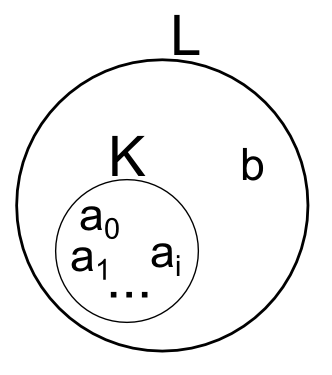
\includegraphics[scale=0.5]{testbovites.png}$$
	Tudjuk a testaxiómákat, tudjuk mi mindent tehetünk $K$ testben. Most tegyük fel, hogy csalni akarunk és úgy szeretnénk tenni, mintha $b$ is $K$ eleme lenne. Hogyan nézne ki akkor a $K$, ha továbbra is szeretnénk, hogy test maradjon?
	
	Ha bevennénk $b$-t, akkor már $b^2$-et is kellene, sőt az összes $b$ hatványt, hogy zártak maradjunk a szorzásra. Sőt, nem csak önmagával, de $K$ beli elemekkel is meg kell tudjuk szorozni a $b$ hatványokat. Tehát biztosan benne kellene lennie a testünkben minden $a_n\cdot b^n+\ldots + a_2\cdot b^2+a_1 \cdot b + a_0$ alakú számnak (bárhogyan is választjuk az $a_i$ elemeket, a fenti ábra esetén tehát annyi pontosítás, hogy minden $a_i$ tetszőleges $K$-beli elem lehet, nem rögzítettek). Ilyen kifejezéssel találkoztunk már, ezek a polinomok. Vagyis ha minden ilyen polinom halmazát tekintem, akkor megkapom a teljes $K$ fölötti polinomgyűrűt a $b$ változóban:
	\[ K[b] = \{a_n\cdot b^n+\ldots + a_2\cdot b^2+a_1 \cdot b + a_0 \}  \]
	Viszont ha továbbra is testet szeretnénk kapni, akkor ezeknek (kivéve a 0 polinomot) inverzére is szükségünk lenne. Tehát szükségünk van a racionális törtfüggvényekre is.
	\begin{defi}
		Legyen $K$ gyűrű és $f(x),g(x)\in K[x]$ és $g(b)\neq 0$. Ekkor az $\dfrac{f(b)}{g(b)}$ elemek halmazát a $K$ gyűrű fölötti \textbf{racionális törtfüggvényeknek} nevezzük. Jelölés:
		\[ K(b) = \left \{ \dfrac{f(b)}{g(b)} \middle | f(x),g(x)\in K[x], g(b)\neq 0 \right \} \]
	\end{defi}
	
	\section{Algebrai, transzcendens, minimálpolinom}
	\begin{defi}
		Legyen $L$ test és $K\leq L$. Ekkor azt mondjuk, hogy $a\in L$ a \textbf{$K$ fölött algebrai}, ha $\exists f(x)\in K[x], f(x)\neq 0$, melyre $f(a)=0$. Egy $a\in \mathbb{C}$ komplex számra ha nem mondjuk mi fölött algebrai, akkor $\mathbb{Q}$ fölött értendő. Ha $a\in L$ nem algebrai, akkor \textbf{transzcendens}.
	\end{defi}
	Például a $\sqrt{2}$ algebrai, mert az $x^2-2$ racionális együtthatós polinomnak gyöke.
	\begin{theo}
		A $\pi$ és az $e$ számok transzcendensek.
	\end{theo}
	Nem bizonyítjuk.
	
	Tegyük fel, hogy $\alpha$ egy algebrai szám $K$ fölött. Ez azt jelenti, hogy $\exists n$, melyre
	\[ f(x)= x^n + a_{n-1} \cdot x^{n-1} + \ldots + a_1\cdot x + a_0  \]
	polinomnak gyöke az $\alpha$. Ez annyit tesz, hogy helyettesítve
	\[ f(\alpha)= \alpha^n + a_{n-1} \cdot \alpha^{n-1} + \ldots + a_1\cdot \alpha + a_0 = 0 \]
	ahonnan $\alpha^n$ kifejezhető az $\alpha$ kisebb hatványaival. Akkor viszont minden $f(\alpha)$ átírható a magasfokú tagok kisebbekre visszavezetésével legfeljebb $n-1$ fokúra.
	
	Ekkor az $\alpha$ változós racionális törtfüggvények halmaza is picit változik, ugyanis feltehető, hogy a számláló és a nevező foka is kisebb mint $n$:
	\[ K(\alpha) = \left \{ \dfrac{f(\alpha)}{g(\alpha)} \hspace{2mm} \middle | \hspace{2mm} f(x),g(x)\in K[x], \hspace{2mm} \deg f,\deg g < n \right \} \]

	Sőt belátható, hogy nem csak magas fokú polinomjai fejezhetők ki $\alpha$-nak kis fokúakkal, de a racionális törtfüggvényei is polinomokkal.
	
	\begin{theo}\label{egyszerubovitesleirasa}
		Ha $\alpha$ algebrai $K$ fölött, akkor $K(\alpha)=K[\alpha]$.
	\end{theo}
	
	Az állítás a gyöktelenítésen múlik, ahogy például az a tény, hogy az $a+b\cdot \sqrt{2}$ alakú számok testet alkotnak. Ott is, illetve még Algebra2-ből a komplexek esetében is az inverz létezésének kérdését gyöktelenítéssel oldottuk meg.
	
	Például miért $a+b\cdot \sqrt{2}$ alakú a $\dfrac{3+\sqrt{2}}{2-\sqrt{2}}$ szám? A nevezőt gyöktelenítve:
	\[ \dfrac{3+\sqrt{2}}{2-\sqrt{2}} \cdot \dfrac{2+\sqrt{2}}{2+\sqrt{2}} = \dfrac{(2+\sqrt{2})\cdot (3+\sqrt{2})}{2} = \dfrac{6+2+3\sqrt{2}+2\sqrt{2}}{2} = \dfrac{8+5\sqrt{2}}{2} = 4 + \dfrac{5}{2} \cdot \sqrt{2} \]
	
	Magát a tételt már nem igazoljuk ebben a fejezetben, de még bevezetünk egy hasznos fogalmat és annak néhány tulajdonságát belátjuk.
	
	\begin{defi}
		Legyen $\alpha$ algebrai $K$ fölött. Az $\alpha$ \textbf{minimálpolinom}jának nevezzük azt a legkisebb fokú, 1 főegyütthatós polinomot, aminek gyöke az $\alpha$. Jelölés: $m(x)=m_\alpha(x)$.
		%\[ m(x) = m_\alpha(x) = \{ p(x)\in K[x] \mid p(\alpha) = 0, \hspace{1mm} \deg p \text{ minimális} \}  \]
	\end{defi}
	\begin{theo}
		Minimálpolinom tulajdonságai:
		\begin{enumerate}
			\item Egyértelműen létezik minimálpolinomja $\alpha$-nak.
			\item $m_\alpha(x)$ irreducibilis $K$ fölött
			\item Minden polinomot oszt, aminek gyöke az $\alpha$: $f(\alpha)=0 \Rightarrow m_\alpha(x) \mid f(x)$
		\end{enumerate}
	\end{theo}
	\begin{proof}
		Az elsőt bizonyítjuk utoljára, mert 2. és 3. felhasználásával egyszerűbb.
		
		\textit{2. biz.:}
		
		Indirekt tegyük fel, hogy $m_\alpha = f(x)\cdot g(x)$, és $f(x)$ és $g(x)$ sem egység. Mivel test fölött vagyunk, egységek a numnulla konstansok, vagyis $f$ és $g$ foka is legalább 1 kell legyen. De mivel fokszámaik összege $m_\alpha(x)$ foka, ezért mindkettő kisebb fokú $m_\alpha(x)$-nél. Helyettesítsünk $\alpha$-t:
		\[ 0 = m_\alpha(\alpha) = f(\alpha) \cdot g(\alpha)  \]
		%ahol $f(\alpha)$ és $g(\alpha)$ mindketten $K(\alpha)$ testbeli elemek, mivel pedig test nullosztómentes, 
		ezért $f(\alpha)=0$ vagy $g(\alpha)=0$. Amennyiben $f(\alpha)=0$, akkor találtunk egy polinomot aminek gyöke az $\alpha$ és foka kisebb mint $m_\alpha(x)$-nek, ez ellentmondás (különben $m_\alpha(x)$ nem lenne minimálpolinom). Hasonlóan $g(\alpha)=0$ is ellentmondást ad.
		
		\textit{3. biz.:}
		
		Test fölött van maradékos osztás, osszuk el $f(x)$-et maradékosan $m_\alpha(x)$-el és lássuk be, hogy $0$ a maradék: $\exists!\ r(x),q(x)\in K[x]$, melyre
		\[ f(x) = m_\alpha(x) \cdot q(x) + r(x) \hspace{4mm} \text{és} \hspace{4mm} \deg r < \deg m_\alpha \hspace{2mm} \text{vagy} \hspace{2mm} r=0  \]
		helyettesítve $\alpha$-t:
		\[ 0 = f(\alpha) = \underbrace{\underbrace{m_\alpha(\alpha)}_{0}\cdot q(\alpha)}_{0} + r(\alpha) = r(\alpha) \]
		Amennyiben $r(x)\neq 0$, akkor találtunk egy $m_\alpha$-nál kisebb fokú polinomot aminek gyöke az $\alpha$, ez ellentmondás lenne ismét. Tehát csakis az lehet, hogy a maradék, $r(x)=0$.
		
		\textit{1. biz.:}
		
		A létezést nem szükséges bizonyítani, hiszen algebrai $K$ fölött az $\alpha$, vagyis van olyan $K$ fölötti polinom, aminek gyöke. Nyilván ezek között minimális fokszámú is van, és ha azt leosztjuk a főegyütthatójával (ezzel a gyökein nem változtatva), akkor megkapjuk a megkívánt 1 főegyütthatónkat is. Nézzük az egyértelműség igazolását.
		
		Legyen $m_1(x)$ és $m_2(x)$	is az $\alpha$ minimálpolinomja. Lássuk be, hogy ők valójában ugyanazok. Nyilván ekkor $m_1(\alpha)=m_2(\alpha)=0$, vagyis a 3. állítás miatt $m_1 \mid m_2$, de hasonlóan $m_2\mid m_1$. Ez csakis úgy lehetséges, ha $m_1 = e\cdot m_2$, ahol $e$ egység. Ráadásul mivel mindkettő minimálpolinom, főegyütthatójuk 1, tehát egészen konkrétan $e=1$ lehetséges csak, azaz $m_1 = m_2$.	
	\end{proof}
	
	Például a $\sqrt{2}$ minimálpolinomja $\mathbb{R}$ és $\mathbb{C}$ fölött is $m_{\sqrt{2}}(x)=x-\sqrt{2}$. Mi a helyzet $\mathbb{Q}$ fölött? Ott $m_{\sqrt{2}}(x)=x^2-2$. Ehhez 2 dolgot kell látni:
	\begin{itemize}
		\item Ennek valóban gyöke a $\sqrt{2}$, hiszen $(\sqrt{2})^2 -2 = 0$
		\item Előző pont miatt a minimálpolinomja $\sqrt{2}$-nek osztja az $x^2-2$ polinomot a bizonyított 3. tulajdonság miatt. Ugyanakkor $\mathbb{Q}$ fölött $x^2-2$ felbonthatatlan (például Schönemann-Eisenstein kritérium $p=2$-vel azonnal látszik).
	\end{itemize}
	
	Hasonlóan $\sqrt[5]{2}$ minimálpolinomja $\mathbb{R}$ fölött $x-\sqrt[5]{2}$, de $\mathbb{Q}$ fölött $x^5-2$, melynek gyöke $\sqrt[5]{2}$, és $p=2$ választással látszik, hogy felbonthatatlan.
	
	
	\chapter{Test és vektortér}
	\section{Testbővítés}
	
	\begin{defi}
		Az $L$ testet a $K$ \textbf{test bővítésének} nevezzük, ha $K$ részteste $L$-nek: $K\leq L$. Jelölés: $L\mid K$.
	\end{defi}

	Például $\mathbb{R}\mid \mathbb{Q}$ és $\mathbb{C} \mid \mathbb{R}$, hiszen $\mathbb{Q}\leq \mathbb{R} \leq \mathbb{C}$.
	
	\begin{pl}
		$ \mathbb{R} \mid \{ a+b\cdot \sqrt{2} \mid a,b\in \mathbb{Q}  \} $.
		Az világos, hogy a jobboldali halmaz részhalmaza $\mathbb{R}$-nek. Azt kellene még belátni, hogy testet is alkot, és akkor igaz volna, hogy $\mathbb{R}$ az ő bővítése:
		\begin{itemize}
			\item Összeadásra zárt: $a+b\sqrt{2}+c+d\sqrt{2} = (a+c)+(b+d)\sqrt{2}$
			\item Szorzásra zárt: $(a+b\sqrt{2})\cdot(c+d\sqrt{2})= (ac+2bd)+(ad+bc)\sqrt{2}$ és $ac+2bd\in \mathbb{Q}$ és $ad+bc\in \mathbb{Q}$
			\item Kommutativitás, asszociativitás, disztributivitás nyilván teljesül.
			\item Nullelem: $0=0+0\sqrt{2}$
			\item Egységelem: $1 = 1+0\sqrt{2}$
			\item Van ellentettje minden elemnek: $a+b\sqrt{2}$ ellentettje $-a-b\sqrt{2}$ is halmazbeli
			\item Van inverze minden nemnulla elemnek: Ha $a+b\sqrt{2}\neq 0$, akkor $a-b\sqrt{2}\neq 0$. Különben ha $a-b\sqrt{2}=0$ volna, akkor két eset lenne lehetséges. Az egyik, hogy $b=0$, ekkor viszont $a=0$ is teljesül, ami ellentmond annak, hogy $a+b\sqrt{2}\neq 0$. A másik, hogy $b\neq 0$, ekkor $\sqrt{2} = \frac{a}{b}$ racionális volna, ami szintén nem lehetséges. Tehát biztosan bővíthetünk konjugálttal:
			\[ \dfrac{1}{a+b\sqrt{2}} \cdot \dfrac{a-b\sqrt{2}}{a-b\sqrt{2}} = \dfrac{a-b\sqrt{2}}{a^2-2b^2} = \dfrac{a}{a^2-2b^2} + \dfrac{-b}{a^2-2b^2} \cdot \sqrt{2} \]
			ahol $\dfrac{a}{a^2-2b^2} \in \mathbb{Q}$ és $\dfrac{-b}{a^2-2b^2} \in \mathbb{Q}$, tehát nemnulla elemeknek létezik inverze.
		\end{itemize}
	\end{pl}

	Ezt az előbb vizsgált furcsa halmazt jelöljük mostantól $\mathbb{Q}(\sqrt{2})$-vel. Belátható, hogy ez a jelölés összhangban van a múlt órai $K(\alpha)$ racionális törtfüggvényekre bevezetett jelöléssel. A racionális törtfüggvények fogalmáig is úgy jutottunk el múlt előadáson, hogy bővíteni szerettünk volna egy testet egy rajta kívüli elemmel és meg akartuk találni a legszűkebb, testaxiómáknak eleget tevő halmazt. Megtehetjük ezt egyszerre több elemmel is. Korábbi tanulmányoknak megfelelően a generálás fogalmát vezetjük be most testelemekre is.
	
	\begin{defi}
		Legyen $L\mid K$ testbővítés és $\alpha, \beta, \ldots \in L$. Ekkor a $K$ és az $\alpha, \beta, \ldots$ elemek által \textbf{generált résztest} az $L$ test legszűkebb olyan részteste, mely $K$-t és az $\alpha, \beta, \ldots$ elemeket is tartalmazza. Jelölés: $K(\alpha,\beta,\ldots)$. Ha csupán egy elemmel bővítünk, azt \textbf{egyszerű} bővítésnek nevezzük\footnote{Az egy elemmel bővítés úgy értendő, hogy $\exists \alpha$ melyre $L\mid K$ bővítésből $L=K(\alpha)$, vagyis a nagyobb test megadható a kisebb egy elemmel való bővítésével. Hiszen mondhatnánk, hogy $\mathbb{Q}(\sqrt{2}) \mid \mathbb{Q} $ bővítés esetén például a $\sqrt{2}$ és az $1+\sqrt{2}$ is bekerült a halmazba (utóbbi az összeadásra való zártság miatt), de jobb szeretnénk mi ezt 1 elemmel való bővítésnek nevezni: $\mathbb{Q}(\sqrt{2},1+\sqrt{2})= \mathbb{Q}(\sqrt{2})$. }. Ennek a jelölése $K(\alpha)$.
	\end{defi}

	Átfogalmazva a generált résztest az adott $K$ testet és $\alpha, \beta, \ldots$ elemeket tartalmazó testek metszete. Persze ellenőrizendő most is a definíció értelmessége: A tavalyiakhoz (generált altér, részcsoport) hasonlóan látható be a következő tétel.
	\begin{theo}
		Testek metszete is test.
	\end{theo}
	
	\begin{all}
		Ha $L\mid K$ testbővítés, akkor $L$ tekinthető egy vektortérnek $K$ felett.
	\end{all}

	Az állítás igazolásához ellenőrizni kellene a 8 vektortér axiómát, melyek nyilván teljesülnek.
	
	\begin{defi}
		Az $L\mid K$ test\textbf{bővítés foka} az $K$ fölötti $L$ vektortér dimenziója: $\dim_K L$. Az $L \mid K$ \textbf{bővítés véges}, ha a foka véges.
	\end{defi}
	
	Például $\dim_\mathbb{R} \mathbb{C} = 2$, hiszen ahogy tavaly is tanultuk az $1$ és az $i$ komplex számok bázist alkotnak. Hasonlóan gondolható végig, hogy $\dim_\mathbb{Q} \mathbb{Q}(\sqrt{2}) = 2$ (az $1$ és a $\sqrt{2}$ bázist alkotnak). Azt is kimondtuk (bizonyítás nélkül) tavaly, hogy $\mathbb{R}$ vektortér $\mathbb{Q}$ fölött végtelen dimenziós. Most analóg módon azt mondhatjuk, hogy $\dim_\mathbb{Q} \mathbb{R} = \infty$, vagyis az $\mathbb{R}\mid \mathbb{Q}$ testbővítés végtelen fokú.
	
	\begin{theo}[Testbővítések fokszámtétele]
		Legyen $K\leq L\leq M$ testbővítések sorozata. Ekkor $\dim_K M = \dim_K L\cdot \dim_L M$, azaz a bővítések foka szorzódik.
	\end{theo}

	\begin{proof}
		Először külön vizsgáljuk ha a jobboldal valamelyike végtelen.
		
		\textit{I. eset:} \hspace{2mm} $\dim_K L = \infty$ \hspace{2mm} vagy \hspace{2mm} $\dim_L M = \infty$
		
		Ha $\dim_K L = \infty$, akkor $L$-ben kiválasztható végtelen sok független vektor. De $L\subseteq M$, vagyis ezek mind benne vannak $M$-ben is, tehát $M$-ben kiválasztható végtelen sok független vektor: $\dim_K M = \infty$
		
		Ha $\dim_L M = \infty$, akkor $M$-ben kiválasztható végtelen sok független vektor. Ez azt jelenti, hogy azokat akármilyen $L$ beli együtthatóval látom el, csakis úgy lehet a lineáris kombinációjuk $0$, ha mindegyik együttható $0$. De akkor ha $L$ helyett annak részhalmazából, $K$-ból választhatok csak együtthatókat, akkor továbbra is csak $0$ együtthatókkal érhetem el, hogy a lineáris kombináció $0$ legyen. Tehát függetlenek maradnak $L$ helyett $K$ felett is a vektorok: $M$-et $K$ felett tekintve van egy végtelen független rendszerem: $\dim_K M = \infty$
		
		\textit{II. eset:} \hspace{2mm} $\dim_K L = s<\infty$ \hspace{2mm} és \hspace{2mm} $\dim_L M = t<\infty$
		
		Legyen $b_1,\ldots,b_s$ bázisa $L$-nek $K$ felett és $c_1,\ldots,c_t$ bázisa $M$-nek $L$ felett. Ekkor azt állítom, hogy
		\[ \{ b_i\cdot c_j \mid 1\leq i\leq s, 1\leq j\leq t  \}  \]
		bázisa $M$-nek $K$ felett. Azt kell belátnunk, hogy független és generátorrendszer. Ha ez megvan, onnan a tétel automatikusan következik, hiszen ez $s\cdot t$ darab vektor, melyek bázist alkotnak, tehát a dimenzió $s\cdot t$.
		
		\begin{itemize}
			\item {Függetlenség:
			
			Legyen
			\[ \sum_{i,j} k_{ij} \cdot b_i c_j = 0  \]
			Azt kell belátnunk, hogy ekkor minden $k_{ij}=0$. Írjuk ki a szummát, hogy lássuk is miről van szó:
			\[ k_{11} \cdot b_1 \color{red} c_1 \color{black} + k_{12} \cdot b_1 c_2 + \ldots + k_{1t} \cdot b_1 \color{blue} c_t \color{black} + k_{21} \cdot b_2 \color{red} c_1 \color{black} + \ldots k_{st} \cdot b_s \color{blue} c_t \color{black} = 0\]
			Csoportosítunk bal oldalon $c_j$-k szerint:
			\[ \underbrace{(k_{11} b_1 + k_{21} b_2 + \ldots + k_{s1} b_s)}_{0} \cdot \color{red} c_1 \color{black} + \underbrace{(\ldots)}_{0} \cdot c_2 + \ldots + \underbrace{(k_{1t} b_1 + k_{2t} b_2 + \ldots + k_{st}  b_s)}_{0} \cdot \color{blue} c_t \color{black} = 0 \]
			Mivel $c_j$-k bázist alkotnak, lineáris kombinációjuk csak akkor lehet $0$, amennyiben minden együttható $0$. Viszont $b_i$-k is bázist alkotnak, ez rájuk is igaz.
			\[ \Rightarrow \hspace{1mm} k_{11}\cdot b_1 + k_{21}\cdot b_2 + \ldots + k_{s1} \cdot b_s = 0 \hspace{2mm} \Rightarrow \hspace{2mm} k_{11}=k_{21}=\ldots=k_{s1} = 0  \]
			Hasonlóan a többi $c_j$ együttható esetében is. Megkaptuk tehát, hogy $\forall k_{ij} = 0$.
		}
			\item {Generálás:
				
			Legyen $m\in M$ tetszőleges. Azt kellene megmutatnunk, hogy léteznek olyan $k_{ij}$ együtthatók, melyekre
			\[ k_{11} \cdot b_1  c_1 + k_{12} \cdot b_1 c_2 + \ldots + k_{st} \cdot b_s c_t = m  \]
			Hát ha nem is tudunk ilyen $k_{ij}$ együtthatókat azonnal, azt tudjuk, hogy $c_1,\ldots,c_t$ generátorrendszer $M$-ben (mert bázis), tehát léteznek olyan $l_1,\ldots, l_t \in L$ elemek, melyekre
			\begin{equation}\label{general}
				l_1\cdot c_1 + \ldots + l_t\cdot c_t = m 
			\end{equation}
			előáll. Továbbá $b_1,\ldots, b_s$ generátorrendszer $L$-ben, tehát bármelyik $l_i\in L$ elem esetén kifejezhető azok lineáris kombinációjával, vagyis léteznek olyan $k_{1i},\ldots, k_{si} \in K$ elemek, melyekre
			\[ l_i = k_{1i} \cdot b_1 + k_{2i} \cdot b_2 + \ldots + k_{si} \cdot b_s  \]
			Helyettesítve (\ref{general}) egyenletbe minden $l_i$ helyére a most kapott kifejezést és elvégezve a szorzásokat, végül $b_i c_j$ elemek lineáris kombinációját kapjuk $K$-beli együtthatókkal. Pont ezt szerettük volna.
		}
		\end{itemize}
	\end{proof}

	\section{Algebrai bővítés}
	Bevezettük előző órán a $K$ test feletti algebrai szám fogalmát. Egy apró észrevétel, hogy $K$ összes eleme algebrai $K$ felett, hiszen $\forall \alpha \in K$ esetén tudunk mutatni olyan $f\neq 0$ polinomot $K$ fölött, melynek gyöke az $\alpha$, például: $x-\alpha$ ilyen. Ezért vizsgálni valamiről, hogy algebrai vagy sem $K$ fölött akkor izgalmas, ha maga az elem nincs benne a $K$-ban.
	
	\begin{theo}\label{masodik}
		Ha $L \mid K$ egy véges bővítés \hspace{1mm} $\Rightarrow$ \hspace{1mm} $\forall l \in L$ algebrai $K$ felett.
	\end{theo}
	\begin{proof}
		Legyen a bővítés foka $\dim_K L = d < \infty$. Tekintsük az $1,l,l^2,\ldots,l^d\in L$ elemeket. Ez $d+1$ darab elem, tehát $L$-beli vektorként tekintve rájuk összefüggő rendszert alkotnak (hiszen $d$ dimenziós $L$, vagyis annál több vektor már biztosan összefüggő). Ekkor viszont $\exists k_0, k_1,\ldots, k_d \in K$ nem mindannyian $0$ skalárok, melyekre
		\[ k_0\cdot 1 + k_1\cdot l + k_2\cdot l^2 + \ldots + k_d\cdot l^d = 0  \]
		ez viszont éppen azt jelenti, hogy a
		\[ k_0 + k_1 \cdot x + k_2 \cdot x^2 + \ldots + k_d \cdot x^d \in K[x]  \]
		polinomnak gyöke az $l$, vagyis $l$ algebrai $K$ felett.
	\end{proof}

	Az előző előadáson kimondtunk egy tételt, hogyan lehet leírni egy test egyetlen algebrai elemmel való bővítését. Az \ref{egyszerubovitesleirasa}. tételt mondjuk ki újra, és most lássuk is be.

	\begin{theo}
		Ha $\alpha$ algebrai $K$ fölött, akkor $K(\alpha)=K[\alpha]$.
	\end{theo}
	\begin{proof}
		Mivel $\alpha$ algebrai, ezért létezik neki minimálpolinomja, jelölje ezt $m_\alpha$. Annak foka legyen $d=\deg m_\alpha$. Tekintsük a következő halmazt:
		\[
			T = \{ a_0 + a_1\alpha + \ldots + a_{d-1} \alpha^{d-1} \mid a_0,a_1,\ldots,a_{d-1} \in K \}
		\]
		Azt fogjuk belátni, hogy $T=K(\alpha)$. Azt mondtuk, hogy $K(\alpha)$ a $K$ test elemeit és az $\alpha$ elemet tartalmazó testek metszete. Ha egy $L$ test tartalmazza $K$ elemeit és $\alpha$-t is, akkor a most definiált halmaz összes elemét is. Tehát a metszet minden egyes tagja tartalmazza $T$-t, akkor végül $K(\alpha)$ is, ezzel beláttuk, hogy $T\subseteq K(\alpha)$.
		
		Elég lesz azt belátnunk, hogy $T$ egy test, hiszen mivel $K(\alpha)$ metszete a $K$ elemeit és az $\alpha$ elemet tartalmazó testeknek, a metszendő elemek egyike $T$, és a metszet mindig részhalmaza a metszendő elemek mindegyikének, így: $K(\alpha) \subseteq T$ teljesülne.
		
		A testaxiómák közül az világos, hogy zárt az összeadásra, van egységelem, ellentett. Szorzat esetén miért lehetünk benne biztosak, hogy $f,g\in T$ esetén $f\cdot g\in T$? A problémát egy dolog jelenthetné, ha megjelenne a szorzatban egy $d-1$-nél magasabb fokú tag is. Mint azonban korábban már láttuk, ekkor $\alpha^d$ kifejezhető volna kisebb hatványok segítségével, hiszen:
		\[ m_\alpha = m_0 + m_1x+\ldots+m_dx^d  \]
		minimálpolinomba helyettesítve $\alpha$-t
		\[ 0 = m_\alpha(\alpha) = m_0 + m_1 \alpha + \ldots + m_d \alpha^d  \]
		egyenletből kifejezhető $\alpha^d$. Hasonlóan magasabb hatványai is az $\alpha$-nak visszavezethetők legfeljebb $d-1$ fokúakra. Ez az oka annak is, hogy $T=K[\alpha]$.
		
		Az igazi kérdés a test tulajdonságok közül tehát a reciprok maradt. Azt kell belátnunk, hogy ha az ellenség ad egy $p(\alpha)\in T$ elemet ($p\neq 0$), akkor mi tudunk neki mutatni egy $q(\alpha)\in T$ elemet, amelyre $p(\alpha)\cdot q(\alpha) = 1$.
		
		Mivel $p(\alpha)\in T$, ezért $\deg p \leq d-1$. Ugyanakkor azt is tudjuk, hogy $m_\alpha$ felbonthatatlan $K$ fölött. Ez azt jelenti, hogy csupán 2 osztója van: 1 és önmaga. Mi lehet akkor $(p,m_\alpha)$? Nem lehet $m_\alpha$, hiszen $\deg p\leq d-1 < d = \deg m_\alpha$. Akkor ez csak az 1 lehet. Az euklideszi algoritmus következménye miatt a legnagyobb közös osztó felírható a polinomok lineáris kombinációjaként: $\exists q_1, q_2 \in K[x]$ melyekre
		\[ p\cdot q_1 + m_\alpha \cdot q_2 = 1  \]
		Ahonnan $\alpha$-t helyettesítve kapjuk, hogy
		\[ p(\alpha) \cdot q_1(\alpha) + \underbrace{\underbrace{m_\alpha(\alpha)}_{0} \cdot q_2(\alpha)}_{0} = 1  \]
		vagyis
		\[ p(\alpha) \cdot q_1(\alpha) = 1  \]
		ami éppen azt jelenti, hogy $q=q_1$ választással megkaptuk $p(\alpha)$ reciprokát.
		
		Rakjuk össze tehát mi mindenünk van: $T=K[\alpha]$, $T\subseteq K(\alpha)$ és $K(\alpha)\subseteq T$. Ezekből láthatóan következik, hogy $K(\alpha) = K[\alpha]$.
	\end{proof}

	\begin{theo}\label{elso}
		Ha $L\mid K$ testbővítés és $\alpha\in L$ algebrai $K$ fölött $\Rightarrow$ a $K(\alpha) \mid K$ bővítés véges, és foka: $\dim_K K(\alpha) = \deg m_\alpha$.
	\end{theo}
	\begin{proof}
		Az előző bizonyításhoz hasonlóan legyen $d = \deg m_\alpha$. Elegendő azt belátnunk, hogy az
		\[ 1, \hspace{2mm} \alpha, \hspace{2mm} \alpha^2, \hspace{2mm} \ldots, \hspace{2mm} \alpha^{d-1}  \]
		egy bázisa $K(\alpha)$-nak és mivel ez $d$ darab elem, így igazolnánk is ezt a tételt. A bázis tulajdonság ekvivalens azzal, hogy segítségével minden egyértelműen áll elő. Ebből az előző bizonyításban már láttuk, hogy $K$ test $\alpha$-val bővített testének minden eleme előáll ezek lineáris kombinációjaként. Elegendő volna az egyértelműséget igazolni.
		
		Tegyük fel, hogy valami kétféleképpen előáll lineáris kombinációként:
		\[ a_0 + a_1\alpha + \ldots + a_{d-1} \alpha^{d-1} = b_0 + b_1\alpha + \ldots + b_{d-1} \alpha^{d-1}  \]
		átrendezve
		\[ (a_0-b_0) + (a_1-b_1) \cdot \alpha + \ldots + (a_{d-1}-b_{d-1})\cdot \alpha^{d-1} = 0 \]
		ahonnan következik, hogy $\forall a_i = b_i$. Hiszen azt látjuk, hogy egy $d-1$ fokú polinom helyettesítési értéke $\alpha$ helyen $0$. Ez akkor csakis a $0$ polinom lehet, különben ellentmondanánk azzal, hogy a minimálpolinom $d$-fokú (találnánk nála kisebb fokút, aminek gyöke az $\alpha$).
	\end{proof}

	\begin{defi}
		Az $L\mid K$ \textbf{algebrai bővítés}, ha $\forall \alpha \in L$ algebrai $K$ felett. Ha egy bővítés nem algebrai, akkor \textbf{transzcendens}nek nevezzük.
	\end{defi}

	\begin{theo}
		Ha $\alpha$ algebrai $K$ felett $\Rightarrow$ a $K(\alpha)\mid K$ algebrai bővítés.
	\end{theo}

	\begin{proof}
		Ez közvetlen következménye a \ref{elso} és \ref{masodik} tételeknek. Ha $\alpha$ algebrai $K$ felett, akkor $K(\alpha)\mid K$ bővítés véges, márpedig véges bővítés esetén $L=K(\alpha)$ speciális esettel a bővebb $K(\alpha)$ test minden eleme algebrai a szűkebb $K$ fölött.
	\end{proof}
	
	\begin{theo}\label{tr_bővítés}
		Minden transzcendens bővítés végtelen dimenziós.
	\end{theo}

	\begin{proof}
		Ha az $L\mid K$ bővítés transzcendens, akkor $\exists \alpha \in L$ elem, amely transzcendens $K$ fölött. Ez azt jelenti, hogy nincs olyan nemnulla polinom, melynek gyöke lenne az $\alpha$.
		
		Ekkor viszont $\alpha$ hatványaiból bármilyen véges sokat véve azok független rendszert alkotnak. Hiszen ha $1,\alpha,\alpha^2,\ldots, \alpha^n$ összefüggő volna, akkor $\exists a_0, a_1, \ldots, a_n\in K$ nem mind nulla számok, melyre
		\[ a_n\alpha^n + a_{n-1}\alpha^{n-1} + \ldots + a_1 \alpha + a_0 = 0 \]
		volna, vagyis az
		\[ a_nx^n + a_{n-1}x^{n-1} + \ldots + a_1 x + a_0 \in K[x] \]
		nemnulla polinomnak gyöke volna az $\alpha$, ami ellentmondás, hiszen feltettük, hogy $\alpha$ transzcendens $K$ fölött.
		
		Viszont ha $\alpha$ hatványaiból akárhányat is véve azok független rendszert alkotnak, akkor találtunk egy végtelen sok elemű független rendszert, a dimenzió végtelen.
	\end{proof}

	Transzcendens bővítés esetén tehát nem elegendő a polinomokkal foglalkoznunk, hanem a racionális törtfüggvények is szerepet kapnak. Előző előadáson látottak alapján azok segítségével írható le egy transzcendens elemmel való bővítés: Például ha a racionális számok halmazát szeretnénk bővíteni a $\pi$ transzcendens elemmel, akkor a
	\[ \mathbb{Q}(\pi) = \left \{ \dfrac{p(\pi)}{q(\pi)} \middle | p,q\in \mathbb{Q}[x], q(\pi)\neq 0 \right \}  \]
	halmaz írja ezt le.

	%1:21 perc
	\section{Mátrixok és egyenletrendszerek}
	Ez a fejezet főleg emlékekről fog szólni, de néhány új fogalommal, állítással is találkoztunk még az óra végén. Átismételtük a mátrix rangjának a fogalmát: oszloprang = maximális független oszlopvektorok száma, sorrang hasonlóan a sorokra. Visszaemlékeztünk, hogy ezek egyenlőek és ráadásul a determinánsranggal is megegyeznek. Ez volt az első új fogalom, mely nem pontosan az általam leírt formában hangzott el, de Freud Róbert: Lineáris algebra című könyvében hasonlóan található meg.
	
	\begin{defi}
		Egy $n\times n$-es mátrix \textbf{aldetermináns}ának nevezzük egy részmátrixának a determinánsát. Vagyis amit úgy kapunk, hogy az eredeti mátrixból választunk valahány oszlopot és ugyanennyi sort, majd a közös részükből képzett mátrix determinánsát vesszük. A választott oszlopok száma az aldetermináns \textbf{rendje}.
	\end{defi}
	
	\begin{defi}[Freud R. 3.4.1.]
		Egy $A$ mátrix \textbf{determinánsrang}ja $r$, ha van olyan $r\times r$-es aldeterminánsa, ami nem nulla, de bármely $r$-nél nagyobb rendű aldeterminánsa (ha egyáltalán van ilyen) már nulla. 
	\end{defi}
	
	Ezután egy szintén tavaly tanult és bizonyított állításról volt szó. A most következő részt a tavalyi jegyzetből másolom.
	
	\begin{theo}[Ismétlés]\label{rangkepter}
		Ha van egy $A\in T^{k\times n}$ mátrix, akkor $r(A)=\dim\mathtt{Im}(A)$, vagyis mátrix rangja megegyezik a hozzátartozó lineáris leképezés képterének dimenziójával.
	\end{theo}
	
	\begin{proof}
		Hogyan szorzunk meg egy mátrixot egy oszlopvektorral jobbról?
		\[\begin{bmatrix}
		\mathbf{a}_1 & \mathbf{a}_2 & \ldots & \mathbf{a}_n
		\end{bmatrix}\cdot \begin{bmatrix}
		\alpha_1 \\
		\alpha_2 \\
		\vdots \\
		\alpha_n \\
		\end{bmatrix}=\alpha_1\cdot \mathbf{a}_1+\alpha_2\cdot \mathbf{a}_2+\ldots+\alpha_n\cdot \mathbf{a}_n\]
		Azt látjuk tehát, hogy a szorzat az eredeti mátrix oszlopvektorainak lineáris kombinációja lesz.
		
		Tekintsük a következő leképezést: Legyen $A$ mátrix rögzített, oszlopvektorai $\mathbf{a}_1,\mathbf{a}_2,\ldots,\mathbf{a}_n$ és tetszőleges $\mathbf{x}$ vektor képe legyen $\varphi(\mathbf{x})=A\cdot \mathbf{x}$. Könnyen látható, hogy ez egy lineáris leképezés. Az kell, hogy összeg képe a képek összege
		\[\varphi(\mathbf{x}_1+\mathbf{x}_2)=A\cdot(\mathbf{x}_1+\mathbf{x}_2)=A\cdot \mathbf{x}_1+A\cdot \mathbf{x}_2 = \varphi(\mathbf{x}_1)+\varphi(\mathbf{x}_2)\]
		és skalárszoros képe a kép skalárszorosa
		\[\varphi(\lambda\cdot \mathbf{x})=A\cdot (\lambda\cdot \mathbf{x})=\lambda\cdot (A\cdot \mathbf{x})=\lambda\cdot \varphi(\mathbf{x})\]
		Márpedig, ha ez egy lineáris leképezés, akkor van neki képtere. Az micsoda?
		
		A képtér azon vektorok halmaza, melyek előállnak képként, vagyis azon $\mathbf{b}$ vektorok amelyekre $\exists \mathbf{x}$ vektor, hogy $A\cdot \mathbf{x}=\mathbf{b}$, vagyis melyek esetén az $A\cdot \mathbf{x}=\mathbf{b}$ lineáris egyenletrendszer megoldható. Másképpen fogalmazva a képtér azon vektorok halmaza, melyek előállnak lineáris kombinációjaként az $\mathbf{a}_1,\mathbf{a}_2,\ldots,\mathbf{a}_n$ vektoroknak, ez pedig éppen az általuk generált altér: $\mathtt{Im}(\varphi)=\langle \mathbf{a}_1,\mathbf{a}_2,\ldots,\mathbf{a}_n \rangle$.
		
		Ha pedig ezek megegyeznek, akkor dimenziójuk is:
		\[ \dim \mathtt{Im}(\varphi) = \overbrace{\dim \langle \mathbf{a}_1,\mathbf{a}_2,\ldots,\mathbf{a}_n \rangle = r(A)}^{\text{def}} \]
	\end{proof}
	
	\begin{theo}
		Az $A\cdot \ve{x}= \ve{b} $ lineáris egyenletrendszernek pontosan akkor létezik megoldása $T$-ben, ha $r(A) = r(A|\ve{b})$, ahol $[A|\ve{b}]$ mátrix alatt az $A$ mátrix $\ve{b}$ oszlopvektorral való kiegészítését értjük. 
	\end{theo}
	
	\begin{proof}
		Pontosan akkor van megoldás, ha $\ve{b}\in \mathtt{Im}(A)$, ami azzal ekvivalens, hogy $\ve{b}$ függ $A$ oszlopvektoraitól. Tehát őt is hozzájuk véve az $\mathtt{Im}(A)$ nem változik, vagyis annak dimenziója (ami a rang) sem változik.
	\end{proof}
	
	Szintén ismétlés, hogy ha adott egy lineáris egyenletrendszernek az egyik megoldása és a homogenizált változat megoldásai, abból hogyan kaphatjuk meg az eredeti összes megoldását.
	
	\begin{all}
		Legyen $A\cdot \ve{x} = \ve{b}$ egyenletrendszer egyik megoldása $\ve{x}_0$, továbbá az $A\cdot \ve{x} = \ve{0}$ egyik megoldása $\ve{h}$. Ekkor $\ve{x}_0+\ve{h}$ is megoldása az eredeti egyenletrendszernek.
	\end{all}

	\begin{proof}
		Azt kell belátnunk, hogy $A\cdot (\ve{x}_0+\ve{h}) = \ve{b}$. Bal oldalt felbontva a zárójelet majd kihasználva, hogy $\ve{x}_0$ partikuláris megoldás, $\ve{h}$ pedig megoldása a homogénnek:
		\[A\cdot (\ve{x}_0+\ve{h}) = A\cdot \ve{x}_0 + A\cdot \ve{h} = \ve{b} + \ve{0} = \ve{b} \]
		ami éppen azt jelenti, hogy $\ve{x}_0+\ve{h}$ megoldása az eredeti egyenletrendszernek.
	\end{proof}
	
	Fontos szerepet játszanak tehát a homogén lineáris egyenletrendszerek is. Visszatérve oda, hogy ha $A\in T^{k\times n}$ mátrixot egy lineáris leképezésnek feleltetjük meg, akkor $A\colon T^n \to T^k$ képez. Azt már láttuk, hogy a leképezés képtere azon vektorok halmaza, melyek esetén $A\cdot \ve{x} = \ve{b}$-nek van megoldása, de mi a magtér?
	
	A magtér azon vektorok halmaza, melyek $\ve{0}$-ba képződnek, vagyis megoldásai az $A\cdot \ve{x} = \ve{0}$ homogén LER\footnote{A továbbiakban a ,,lineáris egyenletrendszer'' kifejezést LER rövidítéssel illetem}-nek. A mag dimenziója és a rang között is kaphatunk összefüggést.
	
	\begin{theo}
		Legyen $A\in T^{k\times n}$, azaz $A$ mátrix egy $T^n \to T^k$ lineáris leképezésnek felel meg. Ekkor $\dim \mathtt{Ker}(A) = n - r(A)$.
	\end{theo}
	
	\begin{proof}
		Írjuk fel a tavalyi félévben, lineáris leképezések magtere és képtere közti kapcsolatra tanult dimenziótételt. $A\colon V_1 \to V_2$ lineáris leképezés esetén
		\[ \dim \mathtt{Ker}(A) + \dim \mathtt{Im}(A) = \dim V_1  \]
		ahol most $V_1 = T^n$, vagyis $n$ dimenziós. A \ref{rangkepter} tétel miatt $\dim \mathtt{Im}(A) = r(A)$, ezeket helyettesítve
		\[ \dim \mathtt{Ker}(A) + r(A) = n \]
		ami éppen a bizonyítandó állítás.
	\end{proof}
	
	\chapter{Szerkesztés}
	\section{Algebrai zártság}
	\begin{defi}
		A $\mathbb{Q}$ és a $\mathbb{Z}_p$ testeket \textbf{prímtest}eknek nevezzük.
	\end{defi}
	A \ref{primtest}. tétel szerint minden testben van tehát egy prímtest. Tehát innentől fogva, ha van egy $K$ testünk, akkor az mindig bővítése egyiknek: $K\mid \mathbb{Q}$ vagy $K \mid \mathbb{Z}_p$. Továbbiakban ha mást nem mondunk, akkor $\mathbb{Q}$ bővítéseiről beszélünk.
	
	Egy $L\mid K$ testbővítés fokát az előző előadáson $\dim_K L$ jelöléssel illettük, a továbbiakban ugyanerre a fogalomra vonatkoznak az $|L : K|$ és a $\dim(L\mid K)$ jelölések is.\footnote{Testbővítések fokszámtételét például nekem könnyebb volt a második jelöléssel megjegyezni. Olyan mintha egy egyszerűsítés miatt esne ki egy osztásból a középső test: $|M:K|=|M:L|\cdot |L:K|$.}
	
	Múlt órán tárgyaltuk az algebrai elemmel való bővítés leírását is:
	\[ K(\alpha) = \{ a_0 + a_1\cdot \alpha + \ldots + a_{n-1} \cdot \alpha^{n-1} \mid n = \deg m_\alpha, \hspace{2mm} a_i\in K  \}  \]
	
	\begin{defi}
		Egy $K$ testet \textbf{algebrailag zárt}nak nevezünk, ha $\forall f\in K[x],\ \deg f\neq 0$ polinomnak van gyöke $K$-ban. 
	\end{defi}

	\begin{theo}
		Ha $K$ algebrailag zárt és $f\in K[x]$, akkor ekvivalensek a következő állítások:
		\begin{enumerate}
			\item $\deg f\geq 1 \Rightarrow \exists \text{ gyöke}$
			\item $\deg f = n \Rightarrow n \text{ gyöke van}$
			\item $f(x)=a_n\cdot (x-\alpha_1)(x-\alpha_2)\ldots(x-\alpha_n)$
			\item Az irreducibilis polinomok pont az 1-fokúak
		\end{enumerate}
	\end{theo}

	\begin{proof}
		Amennyiben $\deg f = 1$, akkor látható, hogy az állítások ekvivalensek. Hiszen ha $f=ax+b$, akkor nyilván van gyöke: $-\frac{b}{a}$, pontosan 1 gyöke van, felírható a gyöktényezős alakja: $f(x)=a\cdot (x-\frac{b}{a})$, és irreducibilis, hiszen bármely test fölötti 1-fokú polinomok irreducibilisek.
		
		Ha pedig $\deg f > 1$ és algebrailag zárt (tehát teljesül az 1. állítás), abból következik a másik három is.
		
		Hiszen ha a foka legalább 1 és van gyöke, akkor emeljük ki gyöktényezőként, ezzel kaptunk egy $\deg f -1$ fokú polinomot, aminek foka még mindig $\geq 1$. Addig ismételgessük ezt a kiemelgetést, amíg 1-fokút nem kapunk. Értelem szerűen ha kezdetben a fok $n$ volt, akkor $n-1$-szer kell ezt megtennünk és végül a maradék tényezőnek is lesz még egy gyöke, tehát összesen $n$ gyöke van $f$-nek.
		
		A kiemelgetések folyamatával előállítottuk a gyöktényezős alakot, és azt is láttuk, hogy ha $f$ foka nagyobb mint 1, akkor mindig kiemelhető elsőfokú tag, tehát $f$ nem irreducibilis. Vagyis pontosan az 1-fokúak irreducibilisek (konstans azért nem lehet irreducibilis, mert test fölött a konstansok egységek vagy a 0 polinom).
	\end{proof}

	\begin{lem}\label{segedtetel}
		$\alpha$ algebrai $K$ fölött $\Leftrightarrow$ $|K(\alpha):K|<\infty$.
	\end{lem}

	\begin{proof}
		Mindkét irányt láttuk már egy korábbi tételben.
		
		\textit{$\Leftarrow$}
		
		Indirekt tegyük fel, hogy $\alpha$ transzcendens. De a \ref{tr_bővítés}. tétel miatt ekkor a $K(\alpha)\mid K$ bővítés végtelen dimenziós lenne, amiről feltettük, hogy véges.
		
		\textit{$\Rightarrow$}
		
		A \ref{elso}. tétel éppen azt mondja hogy ha $\alpha$ algebrai, akkor a $K(\alpha)\mid K$ bővítés véges.
	\end{proof}

	A továbbiakra való tekintettel jegyezzük meg, hogy $K(\alpha,\beta)=K(\alpha)(\beta)=K(\beta)(\alpha)$, hiszen mindegy, hogy egyszerre bővítek $\alpha$ és $\beta$ elemekkel, vagy először $\alpha$, utána $\beta$ elemmel, vagy először $\beta$ majd $\alpha$ elemekkel.

	\begin{theo}\label{becsles}
		Ha $\alpha$ és $\beta$ algebraiak $K$ fölött, akkor $|K(\alpha,\beta):K|\leq |K(\alpha):K|\cdot |K(\beta):K|$.
	\end{theo}

	\begin{proof}
		Az, hogy egyszerre bővítek két algebrai elemmel ugyanaz, mintha külön-külön lépésenként bővítenék velük. Van a $K$ testem és azt először $\alpha$, majd $\beta$ elemmel bővítem: $K(\alpha)\mid K$ majd $K(\alpha)(\beta)\mid K(\alpha)$.
		
		Legyen $K$ fölött az $\alpha$ minimálpolinomja $m_\alpha$, valamint $\beta$ minimálpolinomja $m_\beta$. Ekkor az első $K(\alpha)\mid K$ bővítésem foka $\deg m_\alpha$. A második $K(\alpha)(\beta)\mid K(\alpha)$ bővítés esetén pedig felső korlát $\deg m_\beta$. Hiszen mivel $K \leq K(\alpha)$, ezért ha $K$ együtthatókkal találtunk egy $m_\beta$ polinomot aminek gyöke a $\beta$, akkor annak együtthatói benne vannak $K(\alpha)$-ban is, a minimálpolinom $K(\alpha)$ fölött biztosan nem nagyobb fokú (kisebb lehet, hiszen $m_\beta$ nem biztos hogy irreducibilis $K(\alpha)$ fölött).
		
		Ezzel azt láttuk, hogy $|K(\alpha,\beta):K(\alpha)|\leq |K(\beta):K|$. Használva a testbővítések fokszámtételét már meg is van a bizonyítandó:
		\[ |K(\alpha,\beta):K| = \color{red} |K(\alpha,\beta):K(\alpha)|\color{black} \cdot |K(\alpha):K| \leq \color{red} |K(\beta):K| \color{black} \cdot |K(\alpha):K| \]
	\end{proof}

	Például hogyan mondanánk meg mennyi $d=|\mathbb{Q}(\sqrt{2},\sqrt[3]{2}):\mathbb{Q}|$? Mivel $m_{\sqrt{2}} = x^2-2$ és $m_{\sqrt[3]{2}} =x^3-2$, ezért az előző tétel miatt a bővítés foka $d \leq 2\cdot 3 = 6$.
	
	Közelítsük meg a problémát 2 oldalról. Először képzeljük el, hogy $\sqrt{2}$-vel bővítettük a $\mathbb{Q}$-t, utána hogy azt tovább $\sqrt[3]{2}$-vel. Itt az első bővítés dimenzióját tudjuk: $|\mathbb{Q}(\sqrt{2}):\mathbb{Q}| = 2$. A másodikról most nem tudunk semmit, legyen egyszerűen
	\[d_1 = |\mathbb{Q}(\sqrt{2},\sqrt[3]{2}):\mathbb{Q}(\sqrt{2})| \]
	Ekkor a testbővítések fokszámtétele miatt
	\[ d =  |\mathbb{Q}(\sqrt{2},\sqrt[3]{2}):\mathbb{Q}| = |\mathbb{Q}(\sqrt{2},\sqrt[3]{2}):\mathbb{Q}(\sqrt{2})|\cdot |\mathbb{Q}(\sqrt{2}):\mathbb{Q}| = d_1 \cdot 2  \]

	Hasonlóan végiggondolható, hogy mi történik, ha először $\sqrt[3]{2}$-vel bővítünk:
	\[ d =  |\mathbb{Q}(\sqrt{2},\sqrt[3]{2}):\mathbb{Q}| = |\mathbb{Q}(\sqrt{2},\sqrt[3]{2}):\mathbb{Q}(\sqrt[3]{2})|\cdot |\mathbb{Q}(\sqrt[3]{2}):\mathbb{Q}| = d_2 \cdot 3  \]
	
	Rakjuk össze mit tudunk $d$-ről:
	\[ d\leq 6 \hspace{10mm} d = 2\cdot d_1 \hspace{10mm} d = 3\cdot d_2 \]
	Mivel $2\mid d$ és $3\mid d$, ezért $6\mid d$, ugyanakkor $d$ legfeljebb $6$, tehát $d=6$.

	\begin{defi}
		Jelölés: $\mathbb{A}$ jelöli az \textbf{algebrai számok halmazát}, vagyis
		\[ \mathbb{A} = \{ \alpha \in \mathbb{C} \mid \exists f\in \mathbb{Q}[x],\ f\neq 0,\ f(\alpha) =0  \} \]
	\end{defi}
	
	
	\begin{theo}
		Az algebrai számok algebrailag zárt testet alkotnak.
	\end{theo}
	
	\begin{proof}
		Két lépésben bizonyítunk, először a test tulajdonságot, majd az algebrai zártságot.
		
		\textit{Test biz.:}
		
		Mivel $\mathbb{A}\subseteq \mathbb{C}$, ezért a testaxiómák közül csomó automatikusan teljesül. Hiszen nyilván ha a komplex számok halmazán teljesül, hogy a szorzás asszociatív, akkor ebben a részhalmazban is teljesülni fog. Azt kell tehát csak belátnunk, hogy zárt az összeadásra, szorzásra, ellentett- és reciprokképzésre, vagyis $\alpha,\beta \in \mathbb{A}$ esetén $\alpha+\beta$, $\alpha \cdot \beta$, $-\alpha$ és $\alpha\neq 0$ esetén $\dfrac{1}{\alpha}$ is algebrai. 
		
		Legyenek $\alpha$ és $\beta$ algebrai elemek. A \ref{segedtetel}. lemma szerint ez pontosan azt jelenti, hogy
		\[ |K(\alpha):K| = m < \infty \hspace{5mm} |K(\beta):K| = n < \infty  \]
		Ekkor az előző \ref{becsles}. tétel szerint
		\[ |K(\alpha,\beta):K| \leq n\cdot m < \infty \]
		ami azt jelenti, hogy $K(\alpha,\beta)\mid K$ egy véges bővítés. Véges bővítés esetén a bővebb test minden eleme algebrai a szűkebb fölött a \ref{masodik}. tétel miatt. 
		
		Tehát azt kaptuk, hogy $K(\alpha,\beta)$ minden eleme algebrai $K$ fölött. Ezzel kész is vagyunk, hiszen $K(\alpha,\beta)$ test, ami tartalmazza $\alpha$ és $\beta$ számokat, tehát benne van $\alpha+\beta$, $\alpha\cdot \beta$, $-\alpha$, és $\alpha \neq 0$ esetén $\dfrac{1}{\alpha}$ is.
		
		\textit{Algebrai zártság biz.:}
		
		Azt kell belátnunk, hogy minden $f(x)\in \mathbb{A}[x],\ \deg f \geq 1$ polinomnak van $\mathbb{A}$-beli gyöke.
		
		Legyen $f(x)=x^n+\beta_{n-1}\cdot x^{n-1} + \ldots + \beta_1 \cdot x + \beta_0$, ahol $\forall \beta_i \in \mathbb{A}$. Mivel $\mathbb{A} \subseteq \mathbb{C}$, ezért ez egyben egy komplex együtthatós polinom is. Neki tudjuk, hogy van gyöke $\mathbb{C}$-ben, legyen ez $\alpha$. Azt kellene belátnunk, hogy $\alpha$ algebrai.
		
		Fogjuk meg a $\mathbb{Q}$-t és kezdjük el bővíteni a polinom együtthatóival szépen sorban, ekkor végül kapunk egy $K$ testet
		\[ K = \mathbb{Q}(\beta_0)(\beta_1)\ldots(\beta_{n-1})   \]
		amiről a \ref{becsles}. tétel miatt tudjuk, hogy
		\[ |K:\mathbb{Q}| \leq \prod |\mathbb{Q}(\beta_i):\mathbb{Q}| = |\mathbb{Q}(\beta_0):\mathbb{Q}|\cdot |\mathbb{Q}(\beta_1):\mathbb{Q}|\cdot \ldots \cdot |\mathbb{Q}(\beta_{n-1}):\mathbb{Q}|  \]
		
		Ezt egy picit magyarázom, mert ez a nehezebb gondolat. Ahogy folyamatosan bővítettünk úgy becsülgethetünk is, mindig leválasztunk jobboldalról 1-1 újabb tényezőt:
		\[ |\overbrace{\mathbb{Q}(\beta_0)(\beta_1)\ldots (\beta_{n-2})(\beta_{n-1})}^{K}:\mathbb{Q}| \overbrace{\leq}^{\ref{becsles} \text{. tétel}} |\mathbb{Q}(\beta_0)(\beta_1)\ldots (\beta_{n-2}):\mathbb{Q}|\cdot |Q(\beta_{n-1}):\mathbb{Q}| \leq \ldots  \]
		
		Innen már nem olyan nehéz a bizonyítás. Tudjuk, hogy minden $\beta_i$ algebrai, tehát az összes $|\mathbb{Q}(\beta_i):\mathbb{Q}|$ véges, vagyis a szorzatuk is, tehát $|K: \mathbb{Q}|<\infty$.
		
		Másrészt $|K(\alpha): K|<\infty$, hiszen $\alpha$ algebrai $K$ fölött, mert gyöke az $f\in K[x]$ polinomnak. 
		
		A fokszámtételt használva innen következik, hogy
		\[ |K(\alpha) : \mathbb{Q}| = |K(\alpha):K| \cdot |K:\mathbb{Q}| < \infty  \]
		azaz $|K(\alpha):\mathbb{Q}|$ véges, a \ref{masodik}. tétel szerint ekkor $K(\alpha)$ minden eleme algebrai $\mathbb{Q}$ fölött, tehát $\alpha \in \mathbb{A}$.
	\end{proof}

	\begin{theo}
		Ha $\alpha$ algebrai $\beta$ transzcendens, akkor $\alpha+\beta$ transzcendens és $\alpha\neq 0$ esetén $\alpha\cdot \beta$ is transzcendens.
	\end{theo}

	\begin{proof}
		Indirekt tegyük fel, hogy $\alpha+\beta$ algebrai. Ekkor ebből kivonva az $\alpha$ algebrai számot azt kapnánk, hogy $\beta$. Viszont algebrai számok különbsége is algebrai kellene legyen, $\beta$ ugyanakkor transzcendens, ami ellentmondás.
		
		Hasonlóan $\alpha \cdot \beta = \gamma\in \mathbb{A}$ indirekt feltétellel indulva $ \beta = \dfrac{\gamma}{\alpha}$	adódna, vagyis hogy $\beta$ algebrai.
	\end{proof}

	\section{Euklideszi szerkesztés}
	Ebben a fejezetben az euklideszi-szerkesztést fogjuk algebrai szempontból vizsgálni.
	
	Ismételjük át a lépéseit az euklideszi-szerkesztésnek:
	\begin{itemize}
		\item két ponton húzhatok egy egyenest
		\item két egyenes metszéspontját meg tudom határozni
		\item adott pont körül adott sugárral tudok kört rajzolni
		\item kör és egyenes metszéspontját meg tudom határozni
		\item két kör metszéspontját meg tudom határozni
	\end{itemize}

	Mikor tekintünk egy objektumot megszerkesztettnek? Geometriában úgy csináltuk, hogy \textbf{adott volt néhány pont és meg kellett szerkeszteni néhány új pontot}. De mondhatjuk, hogy egy háromszög már igazából megszerkesztett, ha ismerjük a 3 oldalát, hiszen ha azokat tudjuk, abból meg tudjuk szerkeszteni a háromszöget. Algebrailag tehát a szerkesztést számokkal fogjuk vizsgálni.
	
	Fontos észrevétel: Nincs olyan euklideszi szerkesztési lépés, hogy "húzzunk egy egyenest" csak úgy random! Ahhoz szükséges legalább 2 pont, hogy azt az egyenest meg tudjuk szerkeszteni. Tehát valójában ha kezdetben csak 1 pont adott, akkor azzal semmit nem tudunk csinálni, innentől kezdve feltehető, hogy legalább 2 pontunk kezdetben is van.
	
	Kössünk össze az adott pontok közül 2-t és egyiket $0$-nak nevezzük ($(0,0)$ koordinátákkal látjuk el), másikat $1$-nek nevezzük ($(1,0)$ koordinátákkal látjuk el). A $0$-ból tudunk szerkeszteni a meglévő egyenesre merőleges egyenest, ezzel kaptunk egy koordináta-rendszert. Innentől kezdve gondolkozhatunk végig úgy, hogy minden alakzatunk egy koordináta-rendszerben adott, vagyis jellemezhetjük őket számokkal.
	
	Minden pontot megadhatunk 2 számmal, a koordinátáival. Ha van egy egyenesem: $y=mx+b$, azt is megadhatjuk 2 számmal: meredekség és $y$ tengelymetszet. Kört: $(x-u)^2+(y-v)^2=r^2$ megadhatunk 3 számmal: a $K$ középpontjának 2 koordinátájával és az $r$ sugarával. Vagyis az euklideszi szerkesztés lépéseiben szereplő összes objektum jellemezhető számokkal. Ha távolságot akarunk megadni, azt sem úgy tesszük, hogy 2 pontot adunk meg, hanem egy számot, ami az origotól való távolságot jelenti.
	
	A szerkesztési feladat innentől kezdve úgy néz ki, hogy \textbf{vannak számok, és azokból új számokat kell szerkeszteni}.
	
	\begin{theo}
		A számokkal lehet testműveleteket végezni és gyököt vonni, vagyis ha adott $a$ és $b$ számok megszerkesztettek, akkor meg tudjuk szerkeszteni az $a\pm b$, $a\cdot b$, $b\neq 0$ esetén $\dfrac{a}{b}$ és $\sqrt{a}$ számokat is.
	\end{theo}

	\begin{proof}
		Az összeg szerkesztése könnyű, az $a$ után felmérem a $b$-t (különbség hasonlóan):
		\begin{comment}
			\begin{figure}[h]\begin{center}
			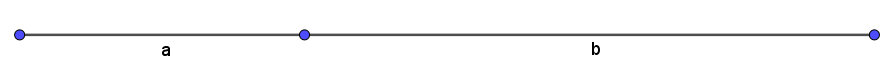
\includegraphics[scale=0.4]{a+b.png}
			\caption{Összeg szerkesztése}
			\end{center}\end{figure}
		\end{comment}
	
		\begin{center}
			$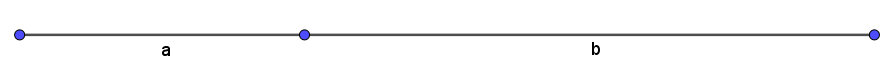
\includegraphics[scale=0.6]{a+b.png}$
		\end{center}
		
		Szorzat szerkesztés a párhuzamos szelők tételén alapszik:
		\begin{center}
			$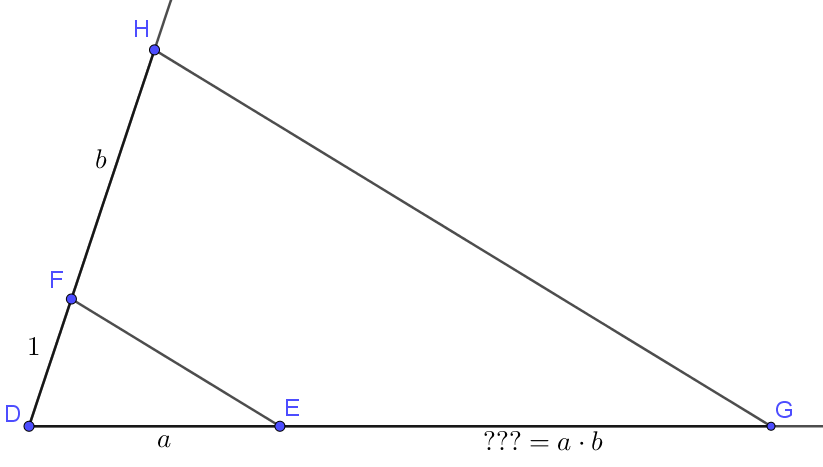
\includegraphics[scale=0.5]{aszorb.png}$
		\end{center}
	
		Hiszen ha
		\[ b = \dfrac{b}{1} = \dfrac{FH}{DF} = \dfrac{EG}{DE} = \dfrac{EG}{a}  \]
		akkor innen $EG=a\cdot b$ következik. Vagyis ha adott $a$ és $b$ (és persze az $1$ távolság is adott, mert van origónk és $(1,0)$ pontunk, aminek segítségével vettük fel a koordináta-rendszert), akkor szorzatuk megszerkeszthető, ha $EF$ egyenessel párhuzamost húzunk $H$ ponton keresztül.
		
		Hányados hasonlóan csak más szereposztással:
		\begin{center}
			$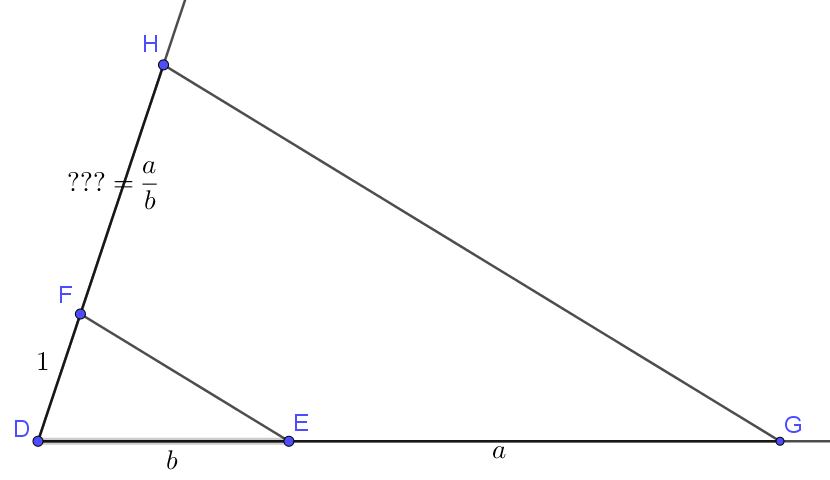
\includegraphics[scale=0.5]{aperb.png}$
		\end{center}
		
		Végül $\sqrt{a}$ megszerkesztése a magasságtétel miatt lehetséges:
		\begin{center}
			$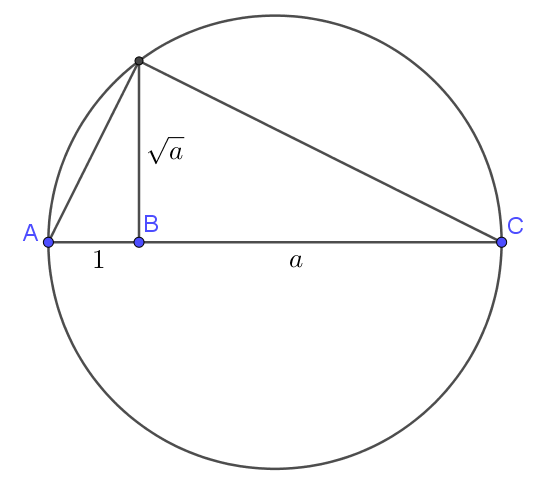
\includegraphics[scale=0.5]{gyoka.png}$
		\end{center}
		Megszerkesztjük $1+a$ szakaszt, majd köré Thalész-kört ($AC$ szakasz felezőpontja a kör középpontja). Merőlegest állítunk $B$ pontban és tekintjük a körrel az egyik metszéspontot. Ha összekötjük $A$ és $C$ pontokkal is, akkor olyan derékszögű háromszöget kapunk, aminek magassága éppen $m=\sqrt{1\cdot a} = \sqrt{a}$.
	\end{proof}

	Az előző állítás azt mondta, hogy ha meg tudjuk szerkeszteni egy $K$ test minden elemét, és egy további $\gamma$ számot is, akkor a $K(\gamma)$ bővebb test összes elemét meg tudjuk szerkeszteni biztosan (tudunk összeadni, kivonni, szorozni, osztani).
	
	\begin{theo}
		Ha megszerkesztettük $K$ test elemeit, akkor egyenesek metszéspontjaként, kör és egyenes metszéspontjaként és körök metszéspontjaként kapható új pont legfeljebb 2-fokú algebrai szám $K$ fölött.
	\end{theo}

	\begin{proof}
		Megvizsgáljuk mindhárom esetet egyesével.
		
		\textit{Egyenesek metszéspontja:}
		
		Van 2 egyenesem (tegyük fel, hogy van metszéspontjuk), egyenleteik ($a,b,c,d\in K$):
		\[
		\begin{cases*}
		y = ax+b \\
		y = cx+d 
		\end{cases*}
		\]
		ekkor kivonva őket egymásból
		\[ 0 = (a-c)x+b-d  \]
		és kifejezve $x$-et
		\[ x = \dfrac{d-b}{a-c} \in K   \]
		és $y = a\cdot \dfrac{d-b}{a-c} +b \in K $, tehát a keletkező metszéspont $K$ testben van, a vele való bővítés 1-fokú.
		
		\textit{Egyenes és kör:}
		
		Van egy egyenesem és egy köröm (megint csak feltéve, hogy kapunk új pontot, tehát van metszéspontjuk), egyenleteik ($a,b,c,m,t\in K$):
		\[
		\begin{cases*}
		x^2+y^2+ax+by+c = 0 \\
		y = mx+t
		\end{cases*}
		\]
		helyettesítve $y$-t az első egyenletbe
		\[ x^2+(mx+t)^2+ax+b(mx+t)+c=0  \]
		rendezve
		\[ \underbrace{(m+1)}_{A}\cdot x^2 + \underbrace{(2mt+a+mb)}_{B}\cdot x + \underbrace{(t^2+ bt +c)}_{C} =0  \]
		bevezetve $A,B,C$ rövidítéseket
		\[ Ax^2+Bx+C = 0 \]
		egyenlethez jutunk, ahonnan $x$-re kapható megoldás
		\[ x = \dfrac{-B\pm \sqrt{B^2-4AC}}{2A}  \]
		ami egy legfeljebb 2-fokú algebrai szám $K$ fölött, hiszen (a megoldóképletet fel se kellett volna írni) gyöke az $Ax^2+Bx+C$ másodfokú polinomnak, aminek együtthatói $K$-beli elemek (tehát minimálpolinomja osztja ezt a másodfokú polinomot, vagyis legfeljebb 2-fokú). 
		
		Ha az $y=mx+t$ egyenletből $x$-et fejezzük ki és ugyanezt végigcsináljuk, akkor látszik, hogy $y$ is legfeljebb 2-fokú algebrai szám.
		
		\textit{Körök metszéspontja:}
		
		Van 2 körünk (metszik egymást), egyenleteik ($a,b,c,d,e,f\in K$):
		\[
		\begin{cases*}
		x^2+y^2+ax+by+c=0 \\
		x^2+y^2+dx+ey+f=0
		\end{cases*}
		\]
		Kivonva az alsót a felsőből
		\[
		\begin{cases*}
		x^2+y^2+ax+by+c=0 \\
		(a-d)x+(b-e)y+c-f=0
		\end{cases*}
		\]
		adódik ahol a második egyenlet már egy egyenes egyenlete, tehát visszavezettük az előző esetre a kérdést, innen $x$ és $y$ már legfeljebb 2-fokú lehet.	
	\end{proof}

	A következőkben azon gondolkozzunk, hogy mi minden szerkeszthető meg, és mi az amiről biztosan meg tudjuk mondani, hogy nem lehetséges. Kezdetben biztosan van az $1$ számunk (ahogy a koordináta-rendszert felvettük: a $(0,0)$ és az $(1,0)$ pontok távolságát neveztük el így). Ebből megszerkeszthető az összes racionális szám.
	
	Vannak a szerkesztési feladatban adott alappontjaink, legyenek ezek $\alpha_1, \alpha_2, \ldots , \alpha_n$. Nyilvánvalóan mivel ezek is adottak, így nem csak $\mathbb{Q}$ elemeit tudjuk megszerkeszteni, hanem annak bővítéseit is az alappontokkal. Ezt nevezem \textbf{alaptest}nek és $K$-val jelölöm most:
	\[ K = \mathbb{Q}(\alpha_1,\alpha_2,\ldots,\alpha_n)  \]
	
	\begin{theo}\label{szukseges}
		Ha $\delta$ megszerkeszthető, akkor $m_\delta$ foka $K$ fölött 2 hatvány.
	\end{theo}

	\begin{proof}
		Ha $\delta$ megszerkeszthető, akkor $\exists\ \gamma_1, \gamma_2, \ldots, \gamma_k$, amely pontokat közvetlenül euklideszi lépésként kapom (tehát előző tétel miatt mindegyik foka 1 vagy 2), melyekkel kibővítve a $K$ testet, abban már benne lesz a $\delta$:
		\[ \delta \in K(\gamma_1,\gamma_2,\ldots,\gamma_k)  \]
		Ez azt is jelenti, hogy ehhez a kibővített testhez aminek eleme $\delta$, ha hozzávenném $\delta$ elemet, nem kapnék bővebb testet, önmaga maradna.
		
		De akkor a nála ,,szűkebb'' $K\leq K(\gamma_1,\gamma_2,\ldots, \gamma_k)$ testhez hozzávéve $\delta$ elemet sem kapnánk bővebb testet:
		\[ K(\delta) \leq K(\gamma_1,\gamma_2,\ldots,\gamma_k)  \]
		A fokszámtétel miatt mivel $K\leq K(\delta)\leq K(\gamma_1,\gamma_2,\ldots,\gamma_k)$:
		\[ |K(\gamma_1,\gamma_2,\ldots,\gamma_k):K| = |K(\gamma_1,\gamma_2,\ldots,\gamma_k):K(\delta)| \cdot |K(\delta):K| \]
		Viszont itt tudjuk a bal oldalról, hogy ha egyesével bővítjük $\gamma_i$-kel a $K$-t, akkor mindig vagy 1-fokú, vagy 2-fokú bővítésünk lesz. Tehát ha végrehajtjuk mind a $k$ darab bővítést, ismét a fokszámtétel miatt ezek a fokszámok összeszorzódnak, vagyis 1-eket vagy 2-eseket szorzunk folyamatosan össze, a szorzat csakis 2-hatvány lehet:
		\[ |K(\gamma_1,\gamma_2,\ldots,\gamma_k):K| = 2^s  \]
		Innen viszont látszik, hogy $|K(\delta):K|$ osztja $2^s$-t, ami azt jelenti, hogy ő maga is 2-hatvány.
	\end{proof}

	Ezzel az állítással kaptunk egy szükséges feltételt a megszerkeszthetőségre. Tehát csakis algebrai számokat tudunk megszerkeszteni, és közülük is csak aminek minimálpolinomja 2-hatvány fokú. Rögtön alkalmazzuk is, vizsgáljunk meg két nevezetes szerkesztési problémát.
	
	\begin{pl}[Kockakettőzés]
		Adott egy kocka, a feladat megszerkeszteni egy olyan kockát, melynek térfogata az övének kétszerese. Mutassuk meg, hogy euklideszi szerkesztéssel ez nem lehetséges!
		
		Legyen az eredeti kocka oldala $a$, ekkor térfogata $V=a^3$. Vagyis nekünk egy olyan kockát kellene szerkeszteni, aminek a térfogata $2\cdot a^3$. Ez viszont azt jelentené, hogy oldala $\sqrt[3]{2}\cdot a$.
		
		Indirekt feltéve, hogy ezt meg tudjuk tenni, azt kapnánk, hogy megszerkeszthető $\sqrt[3]{2}\cdot a$ és $a$ is, akkor hányadosuk $\sqrt[3]{2}$ is. Ez ellentmondás, mert $\sqrt[3]{2}$ minimálpolinomja $\mathbb{Q}$ fölött $x^3-2$, ami azt jelenti, hogy $m_{\sqrt[3]{2}}$ foka $\mathbb{Q}$ fölött $3$, ami nem kettőhatvány.
	\end{pl}

	\begin{pl}[Körnégyszögesítés]
		Adott egy kör, a feladat vele megegyező területű négyzet szerkesztése. Mutassuk meg, hogy euklideszi szerkesztéssel ez nem lehetséges!
		
		Most adott egy kör, sugara legyen $r$. Területe ekkor $r^2\cdot \pi$. A feladatunk olyan $a$ oldalú négyzet szerkesztése, melyre $a^2 = r^2 \cdot \pi$, vagyis $a=r\cdot \sqrt{\pi}$.
		
		Megint csak ha $a$ megszerkeszthető volna, akkor (mivel $r$ adott, így az is megszerkesztett) $\dfrac{a}{r} = \sqrt{\pi}$ is megszerkeszthető volna. Akkor viszont $\sqrt{\pi}\cdot \sqrt{\pi} = \pi$ is, ami ellentmondás, hiszen $\pi$ még csak nem is algebrai (fel sem merül az a kérdés, hogy a foka 2-hatvány vagy sem).
	\end{pl}
	
	\section{Törtek}
	Az egész számokból úgy keletkeztek a racionális számok, hogy szükség volt az osztás műveletére is, ami az egészek köréből kivezet. Sok mindent általánosítottunk már az elmúlt félévekben, most ha mondhatni ilyet, a racionális számok konstrukcióját szeretnénk. Érdemes ebben a fejezetben leírtakat, mint racionális számok tulajdonságait végiggondolni, de általánosabban csinálunk most is dolgokat.
	
	Legyen $R$ egy kommutatív, nullosztómentes gyűrű (vagyis integritási tartomány). Könnyítés kedvéért egyelőre gondolhatunk $\mathbb{Z}$-re. Ennek az $R$ gyűrűnek az elemeiből alkotunk $(a,b)$ rendezett számpárokat, ahol $b\neq 0$. Definiálunk egy relációt is az elemek között.
	
	\begin{defi}
		Az $(a,b)$ és $(c,d)$ rendezett párok akkor és csak akkor állnak relációban, ha $ad=bc$. Jelölés: $(a,b)\sim (c,d)$.
	\end{defi}

	\begin{theo}
		Ez egy ekvivalencia-reláció.
	\end{theo}

	\begin{proof}
		A három szokásos dolgot kell belátni, végig feltesszük, hogy $b,d,f\neq 0$.
		
		\textit{Reflexív:} $(a,b)\sim (a,b)$
		
		Persze, hiszen $ab = ba$, mert kommutatív a gyűrű.
		
		\textit{Szimmetrikus:} $(a,b) \sim (c,d) \Rightarrow (c,d)\sim (a,b)$
		
		Persze, hiszen az első jelentése, hogy $ad=bc$, a másodikhoz pedig az kellene, hogy $cb=da$ ami igaz, mert a szorzás kommutatív és az $=$ reláció szimmetrikus.
		
		\textit{Tranzitív:} $(a,b)\sim (c,d) \hspace{2mm} \text{és} \hspace{2mm} (c,d)\sim (e,f) \Rightarrow (a,b)\sim (e,f)$
		
		Az első kettő jelentése, hogy
		\begin{equation}\label{elsoekvivalencia}
			ad = bc  \hspace{2mm} \text{és} \hspace{2mm} cf=de 
		\end{equation}
		és kellene, hogy $af=be$.
		
		I. eset: $c=0$, ekkor $ad=bc=0$, és mivel nullosztómentes a gyűrű és $d\neq 0$, ezért $a\cdot d = 0 \Rightarrow a=0$. Hasonlóan $de=cf=0$ és $d\neq 0$, ezért $e = 0$. Ekkor viszont kész vagyunk, $af=be=0$ teljesül.
		
		II. eset: $c\neq 0$. Szorozzuk össze a (\ref{elsoekvivalencia}) egyenleteket:
		\[ adcf=bcde  \]
		rendezzük baloldalra és emeljünk ki $cd$-t:
		\[ cd\cdot (af-be) = 0  \]
		mivel itt $c,d\neq 0$, de a test nullosztómentes, ezért $af-be = 0$ következik, ami éppen a bizonyítandó $af=be$.

	\end{proof}
	
	A tavalyiakhoz hasonlóan kapunk tehát ekvivalencia osztályokat, és az egy osztályba tartozó számpárokat tekintjük egyenlőnek. Például ha a gyűrűnk $\mathbb{Z}$, akkor az egyes osztályok képezik a racionális számokat, de ugyanabban az osztályban van a $\dfrac{2}{3} \rightarrow (2,3)$ és $\dfrac{4}{6} \rightarrow (4,6)$, hiszen $2\cdot 6 = 3\cdot 4$.
	
	\chapter{Törtek általánosítása}
	\section{Hányadostest}
	
	%Példák R<=L<=K esetre:
	%R=Z, K=Q, ekkor a második <= kell legyen
	%R=R, K=C, ekkor az első <= kell legyen
	%\begin{theo}
	%	Ha $\exists K$ test, melyre $R<K$, akkor $\exists L$ test, melyre $R\leq L\leq K$ teljesül és $L\cong \mathbb{Q}_R$.
	%\end{theo}

	\begin{defi}
		Legyen $R$ egy kommutatív, nullosztómentes gyűrű. Ekkor értelmezzük az $R$ elemeiből alkotott $(a,b)$ rendezett párok halmazát ($b\neq 0$), továbbá:
		\begin{itemize}
			\item Egy relációt (beláttuk, hogy ekvivalencia-reláció): $(a,b) \sim (c,d) \hspace{1mm} \Leftrightarrow \hspace{1mm} ad=bc$.
			\item Egy szorzás műveletet: $(a,b)\cdot (c,d) = (ac,bd)$.
			\item Egy összeadás műveletet: $(a,b)+(c,d)=(ad+bc,bd)$.
		\end{itemize}
		és az ekvivalenciaosztályok halmazát $R$ \textbf{hányadostest}ének nevezzük. Jelölés: $\mathbb{Q}_R$.
	\end{defi}
	
	\begin{theo}
		A szorzás és az összeadás műveletek jól definiáltak (reprezentáns választásától függetlenek), és $\mathbb{Q}_R$ valóban testet alkot.
	\end{theo}

	\begin{proof}
		\text{ }
		
		\textit{Jól definiált a művelet:} Azt kell megmutatnunk, hogy ha ekvivalens elemeket szorzunk vagy adunk össze, akkor az eredeti szorzattal/összeggel ekvivalens elemet kapunk.
		
		Legyen
		\[ (a_1,b_1)\sim (a_2,b_2) \hspace{3mm} \text{azaz} \hspace{3mm} a_1b_2=b_1a_2 \]
		\[ (c_1,d_1)\sim (c_2,d_2) \hspace{3mm} \text{azaz} \hspace{3mm} c_1d_2=d_1c_2 \]
		
		\textbf{Kellene (összeadáshoz):}
		\[ (a_1,b_1) + (c_1,d_1) \sim (a_2,b_2)+(c_2,d_2)  \]
		elvégezve az összeadást
		\[ (a_1d_1+b_1c_1,b_1d_1) \sim (a_2d_2+b_2c_2,b_2d_2)  \]
		felírva az ekvivalencia definícióját
		\[ (a_1d_1+b_1c_1)\cdot b_2d_2 = b_1d_1 \cdot (a_2d_2+b_2c_2)  \]
		használva a gyűrűben a disztributivitást
		\[ a_1\color{red}d_1\color{blue}b_2\color{black}d_2 + b_1\color{red}c_1\color{blue}b_2\color{black}d_2 = b_1\color{red}d_1\color{blue}a_2\color{black}d_2 + b_1\color{red}d_1\color{blue}b_2\color{black}c_2  \]
		használva a gyűrűbeli kommutativitást
		\[ a_1\color{blue}b_2\color{red}d_1\color{black}d_2 + b_1\color{blue}b_2\color{red}c_1\color{black}d_2 = b_1\color{blue}a_2\color{red}d_1\color{black}d_2 + b_1\color{blue}b_2\color{red}d_1\color{black}c_2  \]
		ami teljesül, hiszen $a_1b_2=b_1a_2$ és $c_1d_2=d_1c_2$.
		
		\textbf{Kellene (szorzáshoz):}
		\[ (a_1,b_1)\cdot (c_1,d_1) \sim (a_2,b_2)\cdot (c_2,d_2)  \]
		elvégezve a szorzást
		\[ (a_1c_1,b_1d_1) \sim (a_2c_2,b_2d_2)  \]
		felírva az ekvivalencia definícióját
		\[ a_1\color{blue}c_1\color{black}\cdot \color{red}b_2\color{black}d_2 = b_1\color{blue}d_1\color{black}\cdot \color{red}a_2\color{black}c_2  \]
		használva a gyűrűben a kommutativitást
		\[ a_1\color{red}b_2\color{black}\cdot \color{blue}c_1\color{black}d_2 = b_1\color{red}a_2\color{black}\cdot \color{blue}d_1\color{black}c_2  \]
		ami igaz, hiszen $a_1b_2=b_1a_2$ és $c_1d_2=d_1c_2$.
		
		\textit{Testaxiómák teljesülése:}
		
		\textbf{Összeadáshoz:}
		\begin{itemize}
			\item{Kommutativitás: $(a,b)+(c,d) = (c,d) + (a,b)$
				elvégezve az összeadást
				\[ (ad+bc,bd) = (cb+da,db)  \]
				ami nyilván igaz, mert $ad+bc=cb+da$ és $bd=db$, hiszen a gyűrűben a szorzás és összeadás kommutatív.
			}
			\item{Asszociativitás: $\Big((a,b)+(c,d)\Big) + (e,f) = (a,b) + \Big((c,d) + (e,f)\Big)$
				elvégezve a ,,belső'' összeadást
				\[ (ad+bc,bd) + (e,f) = (a,b) + (cf+de,df)  \]
				majd a ,,külső'' összeadást
				\[ ((ad+bc)\cdot f + bd\cdot e,bdf) = (a\cdot df + b\cdot (cf+de),bdf)  \]
				használva a gyűrű műveleteinek disztributivitás tulajdonságát
				\[ (adf+bcf+bde,bdf) = (adf+bcf+bde,bdf)  \]
				ami láthatóan megegyezik.
			}
			\item{Nullelem: Ez a $\{(0,a)\}$ ekvivalencia osztály lesz (ahol $0$ a gyűrű nulleleme), hiszen
				\[ (c,d) \overbrace{=}^{\text{kellene}} (0,a) + (c,d) = (0d+ac,ad) = (ac,ad)  \]
				teljesül, hiszen $(c,d)$ és $(ac,ad)$ ugyanabban az ekvivalenciaosztályban vannak, hiszen $(c,d)\sim (ac,ad)$, mivel $cad = dac$.
			}
			\item{Ellentett: Ha van egy $(a,b)$ elemem, annak ellentettje $(-a,b)$,
				hiszen $(-a,b)$ értelmes (mert $b\neq 0$ itt is teljesül, valamint $-a\in R$, mert a gyűrűben van ellentett) és összege $(a,b)$ elemmel a nullelem ekvivalencia osztályát adja:
				\[ (a,b)+(-a,b) = (ab+b\cdot(-a), b^2 ) = (0,b^2) \sim (0,a)  \]
				hiszen $0\cdot a = b^2 \cdot 0 = 0$.
			}
		\end{itemize}
		
		\textbf{Szorzáshoz:}
		\begin{itemize}
			\item{Kommutativitás: $(a,b)\cdot (c,d) = (c,d) \cdot (a,b)$
				elvégezve a szorzást
				\[ (ac,bd) = (ca,db)  \]
				nyilván igaz, mert a gyűrünkben a szorzás kommutatív.
			}
			\item{Asszociativitás: $\Big((a,b)\cdot (c,d)\Big) \cdot (e,f) = (a,b) \cdot \Big((c,d) \cdot (e,f)\Big)$
				elvégezve az első szorzást
				\[ (ac,bd)\cdot (e,f) = (a,b)\cdot (ce,df)  \]
				majd a második szorzást
				\[ (ace,bdf) = (ace,bdf)  \]
				láthatóan megegyezik.
			}
			\item{Egységelem: Az $\{ (e,e) \}$ ekvivalenciaosztály:
				\[ (a,b) \overbrace{=}^{\text{kellene}} (e,e)\cdot (a,b) = (ea,eb)  \]
				teljesül, hiszen $(a,b)$ és $(ea,eb)$ ugyanabban az ekvivalenciaosztályban vannak, hiszen $(a,b)\sim (ea,eb)$, mivel $aeb = bea$.
			}
			\item{Reciprok: Adott $(a,b)\neq (0,b)$ elem reciproka $(b,a)$.
			
				Először is $(b,a)$ értelmes, hiszen ha $a=0$ volna, akkor $(a,b) = (0,b)$ lenne. Továbbá
				\[ (e,e) \overbrace{=}^{\text{kellene}} (a,b)\cdot (b,a) = (ab,ba)   \]
				ez valóban igaz, hiszen $(e,e)\sim (ab,ba)$, mivel $eba=eab$.
			}
		\end{itemize}
		\textbf{Disztributivitás:} $\Big((a,b)+(c,d)\Big) \cdot (e,f) = (a,b)\cdot (e,f) + (c,d)\cdot (e,f)$
		elvégezve a baloldali összeadást
		\[ (ad+bc,bd)\cdot (e,f) = (a,b)\cdot (e,f) + (c,d)\cdot (e,f)  \]
		majd a szorzásokat (használva a gyűrűbeli disztributivitást)
		\[ (ade+bce, bdf) = (ae,bf) + (ce,df)  \]
		majd a jobboldali összeadást
		\[ (ade+bce, bdf) = (aedf + bfce, bfdf)  \]
		valóban megegyezik a két oldal, hiszen
		\[ (ade+bce)\cdot bfdf = bdf\cdot (aed\color{red}f\color{black}+b\color{red}f\color{black}ce)  \]
		mert gyűrűben használva a disztributivitást a jobboldali $f$-ek kiemelésével + kommutativitás használatával látható, hogy a két oldalon ugyanaz áll.		
	
		Sehol nem használtuk fel, hogy a gyűrünk nullosztómentes, akkor minek kötöttük ki? A műveletek értelmességéhez azt is kell látni, hogy nemcsak mindegy melyik elemet választom adott ekvivalencia osztályból, hanem egyáltalán \textbf{létezik} két elem összege, szorzata.
		
		Itt jön képbe a nullosztómentesség, hiszen összeadásnál
		\[ (a,b)+(c,d) = (ad+bc,bd)  \]
		mivel $b,d\neq 0$, ezért $bd\neq 0$, különben nem lenne nullosztómentes a gyűrű. Hasonlóan a szorzás esetében
		\[ (a,b)\cdot (c,d) = (ac,bd)  \]
		eredmény létezik, mert $b,d\neq 0 \Rightarrow bd\neq0$, különben lennének nullosztók.
		
		Összességében láttuk tehát, hogy a definiált műveletek értelmesek és a halmaz testet alkot.
	\end{proof} 
	
	Például az egész ($\mathbb{Z}$) vagy a páros számok ($2\mathbb{Z}$) hányadosteste $\mathbb{Q}$, illetve az egész vagy racionális együtthatós polinomok ($\mathbb{Z}[x]$ és $\mathbb{Q}[x]$) hányadosteste a törtfüggvények ($\mathbb{Q}(x)$).
	
	Az is könnyen látszik, hogy egy test hányadosteste önmaga, vagyis például $\mathbb{Q}$ hányadosteste $\mathbb{Q}$, $\mathbb{R}$ hányadosteste $\mathbb{R}$.
	
	\begin{theo}
		Legyen $R$ egy kommutatív, nullosztómentes gyűrű (vagyis integritási tartomány). Ha $\exists K$ test, melyre $R\leq K$, akkor $\exists L$ test is, melyre $R\leq L \leq K$ úgy, hogy $L\cong \mathbb{Q}_R$.
	\end{theo}
	
	Másképpen úgy is mondhatnánk, hogy van egy gyűrűnk (ami kommutatív, nullosztómentes) és abból akarunk testet csinálni valahogyan. A hányadostesttel lesz izomorf a legszűkebb olyan test, ami tartalmazza a gyűrűt. Hiszen ezen tétel szerint bármely, a gyűrűnél bővebb $K$ testet veszünk, az $R$ és a $K$ között lesz olyan test, ami izomorf $\mathbb{Q}_R$-rel.
	
	A bizonyítás sem így hangzott el előadáson, és a tétel sem (pl.: előadásról a füzetemben $R<L<K$ szerepel, de ha például $K\cong \mathbb{Q}_R$, akkor az utolsó nem lehet szigorú egyenlőtlenség), én végül némi gondolkodás után ennél a verziónál maradtam.
	
	\begin{proof}
		Találnunk kell izomorfizmust $\mathbb{Q}_R$ és $L$ között, vagyis kell egy $\varphi: \mathbb{Q}_R \to L$ művelettartó, bijektív leképezés. Ezek után még azt is meg kell mutatnunk, hogy $R\subseteq L$, valamint $L\subseteq K$. (Mivel mindhárman ugyanarra az összeadás és szorzás műveletre gyűrűt alkotnak, ezért csak a részhalmaz tulajdonságot kell bizonyítani.)
		
		Tekintsük a
		\[ \varphi: \mathbb{Q}_R \to L \hspace{3mm} \text{leképezést, ahol} \hspace{3mm} (a,b)\in \mathbb{Q}_R \hspace{3mm} \text{képe} \hspace{3mm} \varphi\Big((a,b)\Big) = a\cdot b^{-1} = \dfrac{a}{b} \]
		
		\textit{$\varphi$ művelettartó:}
		\begin{itemize}
			\item{\textbf{Összegtartás:} $\varphi\Big((a,b)+(c,d)\Big)=\varphi\Big((a,b)\Big)+\varphi\Big((c,d)\Big)$ ugyanis baloldalt elvégezve az összeadást
			\[ \varphi\Big((ad+bc,bd)\Big)=\varphi\Big((a,b)\Big)+\varphi\Big((c,d)\Big)  \]
			használva $\varphi$ képzési szabályát
			\[ \dfrac{ad+bc}{bd} = \dfrac{a}{b} + \dfrac{c}{d} \]
			valóban teljesül.	
			}
			\item{\textbf{Szorzattartás:} $\varphi\Big((a,b)\cdot (c,d)\Big)=\varphi\Big((a,b)\Big)\cdot \varphi\Big((c,d)\Big)$ ugyanis baloldalt elvégezve a szorzást
			\[ \varphi\Big((ac,bd)\Big)=\varphi\Big((a,b)\Big)\cdot \varphi\Big((c,d)\Big)  \]
			használva $\varphi$ képzési szabályát
			\[ \dfrac{ac}{bd} = \dfrac{a}{b} \cdot \dfrac{c}{d}  \]
			}
			valóban teljesül.
		\end{itemize}
		
		\textit{$\varphi$ bijektív:} 
		\begin{itemize}
			\item{ \textbf{Injektív:} $(a,b)\nsim (c,d) \Rightarrow \varphi\Big((a,b)\Big)\neq \varphi\Big((c,d)\Big)$
			hiszen átírva mindkét oldalát a következtetésnek:
			\[ ad\neq bc \Rightarrow \dfrac{a}{b} \neq \dfrac{c}{d}  \]
			egy igaz következtetés.
			}
			\item{\textbf{Szürjektív:} Adott $a,b\in R$, $b\neq 0$, akkor $\exists (c,d)\in \mathbb{Q}_R$, melyre $\varphi\Big((c,d)\Big)= \dfrac{a}{b}$}
			Nyilván, például $c=a$ és $d=b$ választások jók lesznek.
		\end{itemize}
		Mivel a függvény injektív és szürjektív, ezért bijektív is.
		
		\textit{$R\subseteq L$:}
		
		Legyen $a\in R$ tetszőleges. Ekkor nyilván $a\in L$ is teljesül, hiszen a gyűrűben van egységelem, jelölje ezt $1$. Ekkor viszont $(a,1)\in \mathbb{Q}_R$, melynek képe pedig
		\[ \varphi\Big((a,1)\Big) = \dfrac{a}{1} = a\cdot 1^{-1} = a\cdot 1 = a\in L  \]
		
		\textit{$L\subseteq K$:}
		
		Az $L$ halmaz bármely eleme előáll $a\cdot b^{-1}$ alakban, ahol $a,b\in R$ és $b\neq 0$. Mivel feltettük, hogy $R\leq K$, ezért nyilván $a,b\in K$ és $b\neq 0$ továbbra sem. Ekkor viszont mivel $K$ test, így $b^{-1}\in K$, sőt $a\cdot b^{-1}\in K$. Ezzel $L$ bármely eleméről megkaphatjuk, hogy eleme $K$-nak is, vagyis $L$ valóban részhalmaza $K$-nak.
	\end{proof}
	
	\section{Nevezetes szerkesztési problémák}
	
	\textbf{Emlék:} $\cos{3\alpha} = 4\cos^3\alpha - 3\cos{\alpha}$.
	
	\begin{proof}
		Tekintsük a
		\[ z = \cos\alpha + i\cdot \sin\alpha  \]
		komplex számot. Mi lesz ennek a köbe? Kétféleképpen is hatványozhatunk, egyrészt tudjuk, hogy a szöget kell szorozni $3$-mal, másrészt ténylegesen elvégezhetjük a hatványozást $(a+b)^3$ azonosság segítségével, ekkor:
		\[ z^3 = \cos3\alpha + i\cdot \sin 3\alpha = \cos^3\alpha +3\cos^2\alpha \cdot \sin\alpha \cdot i - 3 \cos\alpha \cdot \sin^2 \alpha - \sin^3\alpha \cdot i  \]
		ahonnan csak a valós részt véve
		\[ \mathtt{Re}(z^3) = \cos 3\alpha = \cos^3 \alpha - 3\cos\alpha \cdot \sin^2\alpha \]
		helyettesítve $\sin^2\alpha = 1 - \cos^2\alpha$-t:
		\[ \cos 3\alpha = \cos^3\alpha - 3\cos \alpha \cdot (1-\cos^2\alpha) = 4\cos ^3 \alpha -3\cos \alpha  \]
		adódik, ami éppen a bizonyítandó.
	\end{proof}
	
	\begin{theo}[Szögharmadolás]
		Nem szerkeszthető meg tetszőleges $\alpha$ szög harmada.
	\end{theo}
	
	\begin{proof}
		A tétel azt mondja ki, hogy nem minden szög harmadát tudjuk megszerkeszteni. Egyeseket azért igen. Például a $180\degree$ harmadát pont meg tudjuk szerkeszteni, mert az $60\degree$. Nekünk csak mutatnunk kell egy példát olyan szögre, melynek harmadát nem lehet megszerkeszteni. Jó példa erre a $60\degree$, azt fogjuk belátni, hogy nem szerkeszthető meg a $20\degree$.
		
		Ha meg tudnánk szerkeszteni ezt a $20\degree$-ot, akkor ott lenne nekünk a szokásos $A=(0,0)$ és $B=(1,0)$ pontunk, és át tudnánk másolni oda ezt a $20\degree$-ot. Ezután szerkeszthetnénk a $AB$ szakasz köré Thalész-kört. Innen a $B$ ponttal szemközti befogó hossza éppen $\cos20\degree$ volna.
		
		\[ 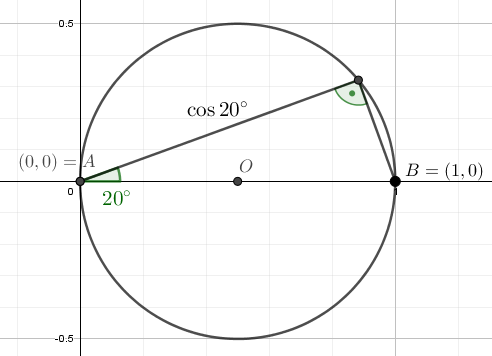
\includegraphics[scale=0.75]{szogharmadolas.png} \]
		
		Tehát elegendő nekünk azt megmutatni, hogy $\cos20\degree$ nem szerkeszthető, innen már következik, hogy $20\degree$ sem. Tudjuk, hogy $\cos 60\degree = \dfrac{1}{2} = \cos (3\cdot 20\degree)$. Felhasználva az emlék azonosságát:
		\[ \dfrac{1}{2} = 4\cdot \cos^3 20\degree -3\cdot \cos 20\degree  \]
		Mit látnak szemeink? A $4x^3-3x-\dfrac{1}{2}$ polinomnak gyöke a $\cos 20\degree$, tehát akkor a $8x^3-6x-1$ egész együtthatós polinomnak is.
		
		Mivel ez egy harmadfokú polinom, ezért pontosan akkor irreducibilis $\mathbb{Q}$ fölött, ha nincs racionális gyöke. Márpedig mivel egész együtthatós(!), alkalmazhatjuk a racionális gyöktesztet, amiből pár próbálkozás után kiderül, hogy nincs racionális gyöke. Tehát az ő nyolcada a $\cos 20\degree$ minimálpolinomja $\mathbb{Q}$ fölött.
		
		Viszont ekkor $|\mathbb{Q}(\cos20\degree):\mathbb{Q}|=3$, ami nem $2$ hatvány, vagyis \ref{szukseges} tétel szerint $\cos 20\degree
		$ nem megszerkeszthető.
	\end{proof}

	\textbf{Emlék:} Az Euler-féle $\varphi$-függvény adja meg $1$-től $n$-ig az $n$-hez relatív prímek számát. Egyben ez határozta meg a primitív egységgyökök számát is, képlete (ha $n=p_1^{\alpha_1}\cdot \ldots \cdot p_k^{\alpha_k}$ kanonikus alakú):
	\[ \varphi(n) = \prod_{i=1}^{k} p_i^{\alpha_i}-p_i^{\alpha_i-1}    \]
	
	\textbf{Emlék:} Az $n$-edik körosztási polinom definíció szerint aminek gyökei az $n$-edik primitív egységgyökök (jelölje őket: $\xi_1,\xi_1,\ldots,\xi_{\varphi(n)}$):
	\[ \varPhi_n(x) = \prod_{i=1}^{\varphi(n)} (x-\xi_i) \]
	Tanultuk (bizonyítás nélkül) Algebra2-ből, hogy a körosztási polinomok 1 főegyütthatós, irreducibilis polinomok $\mathbb{Q}$ fölött.

	\begin{lem}\label{negyseg}
		Legyen $\varepsilon$ egy primitív $n$-edik egységgyök. Ekkor $|\mathbb{Q}(\varepsilon):\mathbb{Q}| = \varphi(n)$.
	\end{lem}

	\begin{proof}
		Az előző emlékből máris következik, hiszen $\varepsilon$ minimálpolinomja $\mathbb{Q}$ fölött éppen $\varPhi_n(x)$, mert ez éppen egy irreducibilis, 1 főegyütthatós polinom, melynek gyöke $\varepsilon$. A képletéből látható, hogy foka $\varphi(n)$.
	\end{proof}

	\begin{lem}\label{egykettedfi}
		A $\cos\left(\dfrac{2\pi}{n}\right)$ algebrai $\mathbb{Q}$ felett és foka $\dfrac{1}{2}\cdot \varphi(n)$, azaz
		\[ \left|\mathbb{Q}\left(\cos \dfrac{2\pi}{n}\right):\mathbb{Q}\right| = \dfrac{\varphi(n)}{2}  \]
	\end{lem}
	
	\begin{proof}
		Tekintsük a $z=1$ komplex számot. Az ő trigonometrikus alakja
		\[ z = 1 =  \cos 2\pi  + i\cdot \sin 2\pi \]
		vegyük az $n$-edik gyökei közül az elsőt, vagyis az $\varepsilon$ primitív egységgyököt.
		\[  \sqrt[n]{1} \to \varepsilon = \cos \dfrac{2\pi}{n}+ i\cdot \sin \dfrac{2\pi}{n}  \]
		
		Az \ref{negyseg} lemmából tudjuk, hogy $|\mathbb{Q}(\varepsilon):\mathbb{Q}| = \varphi(n)$. Fokszámtétel segítségével bontsuk ezt 2 részre:
		\[ |\mathbb{Q}(\varepsilon):\mathbb{Q}| = \varphi(n) = \left |\mathbb{Q}(\varepsilon):\mathbb{Q}\left(\cos \dfrac{2\pi}{n}\right)\right|\cdot \left|\mathbb{Q}\left(\cos \dfrac{2\pi}{n}\right):\mathbb{Q}\right|  \]
		
		Elegendő volna azt belátni, hogy
		\[ \left |\mathbb{Q}(\varepsilon):\mathbb{Q}\left(\cos \dfrac{2\pi}{n}\right)\right| = 2  \]
		
		Ehhez tekintsük az
		\[ x^2 - 2\cdot  \cos \dfrac{2\pi }{n} \cdot  x + 1  \]
		polinomot. Azt állítom, hogy ez $\varepsilon$ minimálpolinomja $\mathbb{Q}\left(\cos \dfrac{2\pi}{n}\right)$ fölött. Amennyiben igazam van kész vagyunk, hiszen ennek 2 a foka. Mi kellene ehhez? Legyen ennek gyöke $\varepsilon$ és legyen irreducibilis.
		
		Mivel $\mathbb{Q}\left(\cos \dfrac{2\pi}{n}\right)$ egy olyan test, mely csak valós számokat tartalmaz, ezért elegendő volna ha belátnánk, hogy nincs valós gyöke a polinomnak, ettől már irreducibilis volna.
		
		Nincs más hátra, nézzük meg a gyökeit! Ha minden jól megy $\varepsilon$ az egyik gyöke, és a másik gyöke sem lesz valós:
		\[ x_{1,2}=\dfrac{2\cdot \cos\left(\dfrac{2\pi}{n}\right) \pm \sqrt{4\cdot \cos^2\left(\dfrac{2\pi}{n}\right) - 4 }}{2} = \cos\left(\dfrac{2\pi}{n}\right) \pm \sqrt{\cos^2\left(\dfrac{2\pi}{n}\right) -1 }  \]
		használva, hogy $1=\sin^2\left(\dfrac{2\pi}{n}\right)+\cos^2\left(\dfrac{2\pi}{n}\right)$:
		\[ = \cos\left(\dfrac{2\pi}{n}\right) \pm \sqrt{-\sin^2\left(\dfrac{2\pi}{n}\right)} = \cos\left(\dfrac{2\pi}{n}\right) \pm i\cdot \sin\left(\dfrac{2\pi}{n}\right)   \]
		ahonnan azt látjuk, valóban $\varepsilon$ és konjugáltja a gyökei a polinomnak, ezzel beláttuk a lemmát.
	\end{proof}

	\textbf{Emlék:} Fermat-számoknak az $F_n = 2^{2^n}+1$ alakú számokat nevezzük, ahol $n\geq 0$ egész. Értelem szerűen Fermat-prím egy olyan Fermat-szám, ami egyben prímszám is, ilyen például az első 5 Fermat-szám, de többről egyelőre nem is tudunk. Algebra1-ből láttuk, hogy ha $p=2^k+1$ alakú szám prím, akkor szükségképpen $k=2^n$, vagyis $p$ ekkor Fermat-prím is.

	\begin{theo}
		Akkor és csak akkor szerkeszthető szabályos $n$-szög, amennyiben
		\[ n = 2^{\alpha} \cdot F_1\cdot F_2 \cdot \ldots \cdot F_t  \]
		kanonikus alakú, ahol minden $F_i$ egy Fermat-prím.
	\end{theo}

	\begin{proof}
		Csak a szükséges feltételt igazoljuk, vagyis hogy ha szerkeszthető $n$ oldalú szabályos sokszög, akkor $n$ a megadott alakú lehet csak (a másik irány nehéz).
		
		A sokszög pontosan akkor szerkeszthető meg, ha megszerkeszthető egy ,,középponti szöge'', vagyis\footnote{azt már megbeszéltük, hogy mindegy, hogy a szöget szerkesztjük meg vagy a koszinuszát} $\cos \frac{2\pi}{n}$.
		
		Mikor szerkeszthető meg $\cos \frac{2\pi}{n}$? Azt tudjuk, hogy foka $\frac{1}{2}\cdot \varphi(n)$ és a \ref{szukseges} tétel miatt csak 2-hatvány fokú számok szerkeszthetők meg, ezért szükségképpen\footnote{bár a feltételünk $\frac{1}{2}\cdot \varphi(n)$-re van, de ha az 2-hatvány, akkor $\varphi(n)$ is muszáj az legyen}
		\[ \varphi(n) = \prod p_i^{\alpha_i} - p_i^{\alpha_i-1}  = \text{2-hatvány} \]
		
		Látható, hogy a $p=2$ prímtényező itt nem sok vizet zavar, rá semmiféle megkötésünk nincs, a kanonikus alak maradék prímeiről kellene belátnunk, hogy csakis Fermat-prím lehet, és csakis az 1 kitevővel.
		
		Tekintsük a többi $p_i$-t. Az ő esetükben $\alpha_i=1$ kell legyen, különben $p_i^{\alpha_i} - p_i^{\alpha_i-1}$ tényezőből kiemelhetnénk $p_i$-t, ami azt jelentené, hogy összességében a szorzat (vagyis $\varphi(n)$) osztható volna $p_i\neq 2$ prímmel. Node $2$-hatvány nem lehet osztható $2$-től különböző prímekkel.
		
		Ha $\alpha_i = 1$, akkor minden $p_i$ ,,szerepe'' a szorzatban: $p_i -1$. Ennek is $2$-hatványnak kell lennie (mert ez továbbra is osztja $\varphi(n)$-t, amiről tudjuk, hogy $2$-hatvány kell legyen). Vagyis valójában $p_i$ egy olyan prím, melyre valamilyen $k$-ra
		\[ p_i -1 = 2^k \hspace{3mm} \Rightarrow \hspace{3mm} p_i = 2^k +1 \]
		az ilyen alakú prímek éppen a Fermat-prímek, kész vagyunk a bizonyítással.
	\end{proof}
	
	Előadás végén még volt szó háromszög szerkesztésről amennyiben adott 2 oldal és 1 szögfelező. Attól függően hogyan vannak megadva az adatok vagy meg lehet szerkeszteni vagy nem a háromszöget. Erre a példára visszatérek a későbbiekben, ha részletesebben tárgyalásra kerülne előadáson.
	
	\chapter{Primitív gyök}
	\section{Kongruencia emlékek}\label{kongruencia_emlekek}
	Ez a fejezet elsősorban emlékeztető néhány Algebra1-ben tanult fogalomról, tételről, ezért szerepel kevés bizonyítás: már elhangzottak régebbi tárgyon vagy nem kell tudni (Kínai maradéktétel).
	
	\begin{theo}\label{linkongr}
		Adott $a,b$ esetén az $ax\equiv b \hspace{1mm} (m)$ lineáris kongruenciának pontosan akkor létezik megoldása (azaz olyan $x$ maradékosztály, mely esetén a kongruencia teljesül), amennyiben $(a,m)\mid b$. Ekkor pedig a megoldások száma $(a,m)$.
	\end{theo}

	\begin{all}
		Egy $R$ gyűrű esetén az egységek\footnote{vagyis ahogy idén félév elején megállapítottuk: az invertálható elemek} halmaza csoport (a szorzásra). Az egységek csoportjának jele mostantól $R^{*}$.
	\end{all}

	\begin{proof}
		Részcsoport tulajdonságot kell vizsgálni: $R^{*}\subseteq R$ zárt a szorzásra és az inverzképzésre. Először is vegyük észre, hogy ez nem egy üres halmaz, mert a gyűrű egységelemét $1$ szimbólummal jelölve, az egyben egység is, tehát benne van a halmazban. Egységek szorzata is egység és minden egységnek van inverze, hiszen ha $e$ egység, akkor mivel $1\in R^{*}$, ezért $e\mid 1$, azaz $\exists f\in R$, melyre $e\cdot f = 1$, ami éppen azt jelenti, hogy az $e$-nek az $f$ az inverze, ráadásul $f$ is egység, tehát $f\in R^{*}$.
		
	\end{proof}
	Például $\mathbb{Z}_m$ esetén az egységek azok az $a\in \mathbb{Z}_m$ elemek, melyeknek van inverze, vagyis melyek esetén az $ax\equiv 1 \hspace{1mm} (m)$ kongruencia megoldható. Ezek \ref{linkongr} tétel szerint éppen azok, melyekre $(a,m)\mid 1$, azaz $(a,m)=1$, vagyis a modulushoz relatív prímek halmaza. Ezeket neveztük Algebra1-ből redukált maradékosztályoknak. Tehát $\mathbb{Z}_m^{*}$ a redukált maradékosztályok halmaza, mely csoportot alkot a szorzásra.\footnote{tavaly is előkerült ez a témakör: 85. oldal, Lagrange-tétel speciális esete az $a^{\varphi(m)}\equiv 1 \hspace{1mm} (m)$ Euler-Fermat-tétel.}
	
	Speciális esete ennek, amikor $m=p$ prím, ekkor $\mathbb{Z}_p^{*} = \mathbb{Z}_p \setminus \{0\} $, hiszen modulo $p$ prím csak a $0$ számnak nincs inverze, az összes többi relatív prím $p$-hez. 
	
	\begin{theo}[Kínai maradéktétel]
		Az
		\[
		\begin{cases*}
		x \equiv a_1 \hspace{1mm} (c_1) \\
		x \equiv a_2 \hspace{1mm} (c_2) \\
		x \equiv a_2 \hspace{1mm} (c_2) \\
		\vdots \\
		x \equiv a_k \hspace{1mm} (c_k) \\
		\end{cases*}
		\]
		szimultán kongruenciarendszernek pontosan akkor létezik megoldása, ha bármelyik 2 kongruenciát kiválasztva az általuk alkotott szimultán kongruenciarendszernek van megoldása, azaz $\forall i,j\colon (c_i,c_j)\mid a_i-a_j$. A megoldás ekkor egyértelmű modulo $[c_1,c_2,\ldots, c_k]$.
	\end{theo}

	\begin{mj}
		Speciális eset: Amennyiben $\forall i,j\colon (c_i,c_j)=1$, akkor egyértelműen létezik megoldás modulo $c_1\cdot \ldots \cdot c_k$.
	\end{mj}
	
	Emlékezzünk vissza \textbf{rend} fogalmára is, mely azóta sok más kontextusban előkerült és hasonló dolgot jelentett mindig: modulo $m$ egy $a$ szám rendje (feltéve, hogy $(a,m)=1$) a legkisebb olyan pozitív egész szám, amely hatványra emelve az $a$ számot $1$-et kapunk. Jelölése: $o_m(a)$.
	
	Azért csak $(a,m)=1$ esetén értelmezzük a rend fogalmát, mert akkor az Euler-Fermat-tétel garantálja, hogy lesz olyan hatványa $a$-nak amely $1$ lesz modulo $m$, például $\varphi(m)$. Látható itt is, hogy jobban szeretünk egy $m=p$ prímszámmal dolgozni, hiszen ekkor $(a,p)=1$ bármely $a\neq 0$ elemre, vagyis minden nemnulla elemnek van rendje.
	
	Tudjuk, hogy osztja a ,,jó'' kitevőket, vagyis $a^c \equiv 1 \ (m) \Leftrightarrow o_m(a)\mid c$. Mivel $\varphi(m)$ egy jó kitevő, ezért $o_m(a)\mid \varphi(m)$. További fontos tulajdonságai, hogy $a^b\equiv a^c\ (m) \Leftrightarrow b\equiv c \ (o_m(a))$, és az $a$-nak $o_m(a)$ darab modulo $m$ páronként inkongruens hatványa létezik.
	
	\begin{pl}\label{maxelemrend}
		Tudjuk, hogy $\varphi(100)=\varphi(2^2\cdot 5^2)=\varphi(2^2)\cdot \varphi(5^2)=(2^2-2^1)\cdot(5^2-5^1)=2\cdot 20 = 40$ és $(7,100)=1$, ezért az Euler-Fermat-tétel miatt
		\[ 7^{40} \equiv 1 \ (100)  \]
		De hasonlóan $\varphi(25)=20$ és $\varphi(4)=2$, ezért
		\[ 7^{20}\equiv 1 \ (25) \hspace{5mm} \text{és} \hspace{5mm} 7^2\equiv 1 \ (4)  \]
		ahonnan a második kongruenciát $10$-edik hatványra emelve
		\[
		\begin{cases*}
		7^{20}\equiv 1 \ (25) \\
		7^{20}\equiv 1 \ (4) \\
		\end{cases*}
		\]
		De mivel $(4,25)=1$, ezért az
		\[
		\begin{cases*}
		x\equiv 1 \ (25) \\
		x\equiv 1 \ (4) \\
		\end{cases*}
		\]
		szimultán kongruenciarendszernek a kínai maradéktétel szerint egyértelműen létezik megoldása modulo $25\cdot 4 = 100$, márpedig az $1$ elem teljesíti ezt, vagyis $x\equiv 1 \ (100)$. Jelen esetben $7^{20} \equiv~1 \ (100)$. Ez egyben azt is jelenti, hogy $o_{100}(7)\neq 40$, mert találtunk nála kisebbet, de mivel osztja a ,,jó'' kitevőket, ezért $o_{100}(7)\mid 20$.
		
		%Egyébként $o_{100}(7)=4$, mert $7\not\equiv 1\ (100)$, $7^2=49\not\equiv 1 \ (100)$, de  $7^4=49^2=(50-1)^2=50^2-2\cdot 50 + 1 \equiv 1 \ (100)$.
		
		Egyébként bármely $(a,100)=1$ esetén ugyanez elmondható lett volna, tehát modulo $100$ egyetlen olyan elem sincs, aminek a rendje $40$.
	
	\end{pl}	

	Emlékezzünk még meg a renddel kapcsolatban arról az összefüggésről, mely egy elem rendje és hatványai rendje között áll fenn, és mely szintén előkerült korábbi tanulmányok során:
	\begin{theo}\label{gi}
		Egy $g$ elem $i$-edik hatványának rendje az elem rendjének ismeretében:
		\[ o(g^i) = \dfrac{o(g)}{(i,o(g))}  \]
	\end{theo}
	
	
	\section{Primitív gyök}
	
	Mivel $o_n(a)\mid \varphi(n)$, ezért nyilvánvaló, hogy a maximális elemrend $\varphi(n)$. A \ref{maxelemrend} példában láttuk, hogy ez bizony jóval kisebb is lehet. A kérdés, hogy van-e olyan elem, aminek a rendje éppen $\varphi(n)$.
	
	\begin{defi}
		Egy $a$ számot \textbf{primitív gyök}nek nevezünk modulo $n$, ha $o_n(a)=\varphi(n)$.
	\end{defi}

	Láttuk, hogy modulo $100$ nem létezik primitív gyök, hiszen $7$ helyett bármelyik másik, $100$-hoz relatív prím esetén megállta volna helyét a gondolatmenetünk (nem relatív prímek esetén pedig a rend értelmezve sincs).

	\begin{theo}
		Modulo $n$ pontosan akkor létezik primitív gyök, amennyiben $n=2$ vagy $n=4$ vagy ($\exists p>2$ prím és $\alpha>0$, melyre) $n=p^{\alpha}$ vagy $n=2\cdot p^{\alpha}$. 
	\end{theo}
	
	A tétel $n=2$ esetén nyilvánvaló, mert $\varphi(2)=1=o_2(1)$, hasonlóan $n=4$ esetén $\varphi(4)=2^2-2^1 = 2 = o_4(3)$, hiszen $3^2\equiv 1\ (4)$, de $3^1\not \equiv 1 \ (4)$. Az állítást ezen kívül csak $n=p$ esetre fogjuk belátni, de először szükségünk lesz ehhez egy lemmára.
	
	\begin{lem}\label{lemma}
		$\displaystyle \sum_{d\mid n} \varphi(d) = n$.
	\end{lem}

	Vagyis ha veszem egy szám osztóit, mindegyiknél a $\varphi$ helyettesítési értékét, majd összeadom, akkor megkapom az eredeti számot. Például 6 osztói: $1,2,3,6$, azaz a tétel szerint
	\[ \varphi(1)+\varphi(2)+\varphi(3)+\varphi(6)= 1+1+2+2 =6  \]

	Kétféle bizonyítást is mutatunk, az első bizonyos értelemben ,,elemibb'' lesz.

	\begin{proof}
		Tekintsük a következő törteket:
		\[ \dfrac{1}{n}, \hspace{3mm} \dfrac{2}{n}, \hspace{3mm} \dfrac{3}{n}, \hspace{3mm} \ldots, \hspace{3mm} \dfrac{n}{n} \]
		Kétféleképpen is meg fogjuk számolni, hogy hány darab tört ez. Egyrészt ez szemlátomást $n$ darab tört. Hurrá! A feladat felével meg is vagyunk, már csak a $90\%$-a van hátra.
		
		Egyszerűsítsük az összes törtet innen. Ha van egy $\frac{k}{n}$ törtünk, akkor hogyan egyszerűsítjük azt? Leosztjuk a számlálót és nevezőt is a legnagyobb közös osztójukkal. Vagyis 
		\[ \dfrac{k}{n} = \dfrac{\hspace{1mm} \frac{k}{(k,n)} \hspace{1mm}}{\frac{n}{(k,n)}} = \dfrac{a}{d} \]
		alakot kapunk, ahol $(a,d)=1$ és $\frac{n}{(n,k)} = d \Leftrightarrow n = (n,k)\cdot d$ azaz $d\mid n$.
		
		Adott $d$ esetén hányféle lehet $a$ értéke? Ahány relatív prím választható $d$-hez. Ez éppen $\varphi(d)$. Nincs más dolgunk, mint hogy végighaladjunk az $n$ összes $d$ osztóján és mindegyikre összegezzük $\varphi(d)$ értéket, ezzel megkapjuk a felírt törtek számát, amiről láttuk, hogy $n$ darab. Éppen ezt mondja a lemma.
	\end{proof}

	\begin{proof}
		Tekintsünk egy $n$ elemű ciklikus csoportot\footnote{egyetlen elemének $n$ különböző hatványából áll, lásd: Algebra3 jegyzet, 7.4. fejezet}, amelyet egy $g$ elem generál: $G = \langle g \rangle$. Ekkor tudjuk, hogy $g$ elemnek $n$ különböző hatványa van, tehát $o(g)=n$.
		
		Hány olyan eleme van a csoportnak\footnote{feltesszük, hogy van egyáltalán ilyen rendű eleme, ha nincs akkor nyilván 0}, aminek a rendje éppen $d$? A csoport elemei $g^i$ alakúak és most olyan $i$ számot keresünk, amire $o(g^i)=d$. Hogyan néz ki az elemek rendje az előző fejezet végén lévő képlet alapján?
		\[ d =  o(g^i) = \dfrac{o(g)}{(i,o(g))} = \dfrac{n}{(i,n)}  \]
		azt látjuk tehát, hogy 
		\[ d = \dfrac{n}{(i,n)} \hspace{2mm} \Leftrightarrow \hspace{2mm} d\cdot (i,n) = n \hspace{2mm} \Leftrightarrow \hspace{2mm} (\color{red}d\cdot i\color{black},d\cdot n) = \color{red}n\color{black}  \]
		Egyrészt a középső egyenlőségből következik, hogy $d\mid n$, ezt mindjárt használni fogjuk.
		
		Valamint látható, hogy $\color{red}n\color{black}\mid \color{red}d\cdot i\color{black}$, ami azt jelenti, hogy $\exists j$, melyre $n\cdot j = d \cdot i$. Mivel $d\mid n$, ezért leoszthatunk vele
		\[ \dfrac{n}{d} \cdot j = i  \]
		Azt kaptuk tehát, hogy ez csakis olyan hatványokra igaz, amelyek kitevője $\dfrac{n}{d}\cdot j$ alakú. Helyettesítve $i$ helyére 
		\[ (d\cdot \dfrac{n}{d} \cdot j, d\cdot n) = n  \]
		vagyis azt kaptuk, hogy
		\[(n \cdot j,n \cdot d) = n\cdot (j,d) = n \]
		egyszerűsítve $n$-nel: $(j,d)=1$. Ez azt jelenti, hogy annyi féleképpen választható meg $j$ (majd abból következően $i$ is), ahány relatív prím létezik $d$-hez, ez éppen $\varphi(d)$.
		
		Tehát a $d$ rendű elemek száma $\varphi(d)$. A csoport elemeit megszámolhatjuk úgy, hogy egyesével összegezzük, hogy a különböző rendű elemeiből hány van. Tehát képezve $\displaystyle \sum_{d\mid n} \varphi(d)$ összeget megkapjuk a csoport elemszámát, amiről tudjuk, hogy $n$.
	\end{proof}
	Az előző bizonyítás vége egy picit be tud minket csapni: "Tehát a $d$ rendű elemek száma $\varphi(d)$". Ne feledjük el, hogy itt ezt a $d$ számot a csoport elemszámának különös módon történő megszámolásához akartuk felhasználni, tehát feltehettük, hogy csak olyan $d$ számokkal foglalkozunk, amelyek tényleg előállnak valamely elem rendjeként! Láttuk például, hogy modulo $100$ egyetlen elem sincs, aminek a rendje $40$ lenne.
	
	\begin{theo}\label{tudnikell}
		Ha $p$ prím, akkor modulo $p$ létezik primitív gyök.
	\end{theo}

	\begin{proof}
		A bizonyítás során tehát végig $\mathbb{Z}_p$-ben vagyunk. Mit tudunk elmondani, ha tudjuk 2 elemről, hogy rendjeik megegyeznek? Például legyen $o(a)=d$ és $o(b)=d$. Mik lesznek ekkor az $x^d-1\in \mathbb{Z}_p[x]$ polinom gyökei?
		
		Láthatóan gyöke az $1$. Aztán $a$ is, hiszen $a^d\equiv 1 \ (p)$. Hasonlóan gyöke $a^2$, mert \[ (a^2)^d -1 = (a^d)^2-1 \equiv 1^2-1 \equiv 0 \ (p) \]
		Hasonlóan látható, hogy $a$-nak az összes különböző hatványa gyöke. Mivel $a$ rendje a páronként inkongruens hatványainak számával egyezik meg, ezért
		\[ 1, \hspace{3mm} a, \hspace{3mm} a^2, \hspace{3mm} \ldots,  \hspace{3mm} a^{d-1}  \]
		$d$ különböző hatványa $a$-nak, tehát ők biztosan gyökei a polinomnak.
		
		Igen ám, de annak más gyöke nincs is rajtuk kívül, hiszen a polinomunk a $\mathbb{Z}_p$ test fölötti polinom, tehát legfeljebb annyi gyöke lehet, amennyi a foka, ami jelen esetben $d$.
		
		De vegyük észre, hogy mivel $o(b)=d$, ezért $b^d-1\equiv 0 \ (p)$, ami azt jelenti, hogy $b$ is gyöke a polinomnak. Ez csak akkor lehetséges, ha $\exists i$, melyre $b = a^i$. Mi történne ha most akarnánk kiszámolni $b$ rendjét?
		\[ d = o(a) = o(b) = o(a^i) = \dfrac{o(a)}{(i,o(a))}  = \dfrac{d}{(i,d)}  \]
		összeolvasva az elejét és a végét: $d=\dfrac{d}{(i,d)}$ ahonnan $(i,d)=1$.
		
		Most is azt látjuk tehát, hogy ha van $d$ rendű elem, akkor abból $\varphi(d)$ darab van. Vezessünk most be egy függvényt, hogy lekezeljük ezt a ,,ha van akkor'' problémát:
		\[ \psi(d) = \begin{cases*}
		\varphi(d) & \text{ha van $d$ rendű elem} \\
		0 & \text{különben}\\
		\end{cases*}  \]
		
		Na most végre először legálisan mondhatom ki, hogy a $d$ rendű elemek száma $\psi(d)$. Innen igazából annyit szeretnénk bizonyítani, hogy $\psi(p-1)>0$, hiszen ekkor létezik $\varphi(p) = p-1$ rendű elem, vagyis primitív gyök modulo $p$.
		
		Rögtön egy \textbf{fontos megállapítás}: $\varphi(d)\geq \psi(d)$, hiszen amilyen $d$-re van $d$ rendű elem, ott közös az értékük, különben pedig $\varphi(d)\geq 0 = \psi(d)$ igaz.
		
		Másik észrevétel: Minden elemnek van rendje! Pontosabban majdnem mindnek, a $0$-nak nincs. De rajta kívül minden $a$-ra igaz, hogy $(a,p)=1$, tehát értelmezzük rá a rend fogalmát. Azt is tudjuk, hogy mindegyik elem rendjére igaz, hogy $o(a)\mid \varphi(p) = p-1$. Vagyis ha végighaladnánk $p-1$ osztóin és megszámolnánk, hogy hány olyan elem van, aminek éppen az a rendje, akkor megszámolnánk $\mathbb{Z}_p$ elemeit a $0$ kivételével, vagyis $p-1$ elemet számolnánk. Képletre fordítva a rizsát:
		\[ \displaystyle \sum_{d\mid p-1} \psi(d) = p-1  \]
		
		Na most rakjunk össze mindent! Becsüljünk minden $\varphi(d)$-t alulról $\psi(d)$-vel:
		\[ \overbrace{p-1 = \displaystyle \sum_{d\mid p-1} \varphi(d)}^{\ref{lemma}\text{ lemma}} \geq \displaystyle \sum_{d\mid p-1} \psi(d) = p-1  \]
		Hiába becsültünk, nem lett kisebb ahonnan elindultunk. Ez csakis akkor lehetséges, ha valójában nem is történt becslés és $\forall d$ esetén $\psi(d)=\varphi(d)$. De akkor konkrétan $\psi(p-1) = \varphi(p-1)>0$. Ezt akartuk.
	\end{proof}
	
	\begin{pl}
		Adjunk meg modulo $7$ egy primitív gyököt!
		
		Mivel a $7$ prím, ezért meg tudjuk ezt tenni, például a $3$ megfelelő lesz. Mivel $\varphi(7)=6$, ezért $6$ osztói jöhetnek szóba amikor $3$ rendjét keressük, de $3^2=9\equiv 2 \ (7)$, illetve $3^3 = 27 \equiv -1 \ (7)$. Tehát $o_7(3)=6$, vagyis a $3$ primitív gyök modulo $7$.
	\end{pl}

	Primitív gyök kereséskor segítségünkre lehet, ha ismerjük egy szám különböző hatványait. Ezeket a könnyebb átláthatóság kedvéért egy táblázatban rögzíthetjük, melynek felső sorába kerül a kitevő, alsóba pedig a hatvány.
	
	Készítsünk a $2$-höz modulo $23$ egy ilyen táblázatot! Annyi oszlopunk lesz, ahány különböző hatvány, vagyis ami $2$-nek a rendje. Tehát addig kell írjuk az oszlopokat, amíg az alsó sorban $1$-est nem kapunk.
	
	Számolás közben könnyíti a munkánkat, hogy elegendő modulo $23$ számolni, tehát például $2^5=32 \equiv \color{red}9\color{black}\ (23)$. Ezután $2^6=2\cdot 2^5 \equiv 2\cdot 9 = \color{blue}18\color{black}\ (23)$.
	
	\begin{center} \begin{large}
		\begin{tabular}{ | c | c | c | c | c | c | c | c | c | c | c | c | }
			\hline
			$\mathbf{n}$ & 1 & 2 & 3 & 4 & 5 & 6 & 7 & 8 & 9 & 10 & 11 \\ 
			\hline
			$\mathbf{2^n}$ & 2 & 4 & 8 & 16 & \color{red}9 & \color{blue}18 & 13 & 3 & 6 & 12 & 1 \\
			\hline   
		\end{tabular}
	\end{large} \end{center}

	A táblázatból közvetlenül leolvasható, hogy $o_{23}(2)=11\neq 22=\varphi(23)$, tehát a $2$ nem primitív gyök modulo $23$. Ennél azonban sokkal több is látszik. A táblázat alsó sorában szereplő számok egyike sem lehet primitív gyök modulo $23$.
	
	Ugyanis ha veszek egy számot, ami előáll $2$-nek egy hatványaként, akkor annak már a $11$-edik hatványa biztosan $1$ lesz, hiszen bármelyik $a$ számot is venném ki az alsó sorból, létezne olyan $i$, melyre $a\equiv 2^i\ (23)$. Ekkor
	\[ a^{11}\equiv (2^i)^{11} = (2^{11})^i \equiv 1^i = 1\ (23) \]
	
	Ezzel kizártunk egy rakás számot, ami biztosan nem primitív gyök modulo $23$. Persze ez a táblázat másra is használható. Tudjuk, hogy a $2$-nek az összes különböző hatványa előfordul. Ezek után könnyen leolvasható, hogy például hanyadik hatványa lesz $2$-nek $9$: az $5$. hatványa.
	
	Ez az utóbbi kérdés a logaritmus fogalmára emlékeztet minket. Mintha egy olyan számot keresnénk, melyre $2^x=9$. Ezt valós számokra úgy oldanánk meg, hogy $x=\log_2 9$. Ezen intuíció alapján definiálhatnánk maradékosztályokra is a logaritmus fogalmát. A gond itt az volna, hogy például mi a helyzet $\log_2 5$ értékével? Modulo $23$ nem áll elő $2$-hatványként az $5$. Tehát itt nem csak a $0$ maradékosztályt kellene kizárjuk. Ennek érdekében ezt a fogalmat\footnote{Freud: Számelmélet könyv 3.4.1 Definíció} primitív gyökökre szokás értelmezni, és csak amennyiben a modulus prímszám, a fogalom neve \textbf{diszkrét logaritmus} vagy \textbf{index}.
	
	Ettől függetlenül a könnyebb áttekinthetőség kedvéért mi nyugodtan megfordíthatjuk a táblázat két sorát és ,,sorba rendezhetjük'' a maradékosztályokat attól függetlenül, hogy a $2$ nem primitív gyök modulo $23$.
	
	\begin{center} \begin{large}
			\begin{tabular}{ | c | c | c | c | c | c | c | c | c | c | c | c | }
				\hline
				$\mathbf{2^n}$ & 1 & 2 & 3 & 4 & 6 & 8 & 9 & 12 & 13 & 16 & 18 \\
				\hline
				$\mathbf{n}$ & 11 & 1 & 8 & 2 & 9 & 3 & 5 & 10 & 7 & 4 & 6 \\ 
				\hline   
			\end{tabular}
	\end{large} \end{center}
	
	Hogyan tudnánk mondani egy primitív gyököt modulo $23$? Láttuk, hogy a $2$ nem volt jó, mert $11$. hatványa már $1$. De például jó lenne nekünk a $-2$. Hiszen $o_{23}(-2) \in \{ 1, 2, 11, 22  \}$, ahonnan az első 2 eset láthatóan nem igaz. Itt viszont már azt is láthatjuk, hogy a $11$. hatványa sem lesz egy, hiszen
	\[ (-2)^{11} = (-1)^{11} \cdot 2^{11} \equiv -1\cdot 1 \equiv -1\ (23)  \]
	tehát a $-2\equiv 21$ egy primitív gyök modulo $23$.
	
	Neki könnyű felírni ezt a fajta táblázatát is, hiszen hatványozása ugyanúgy zajlik ahogy $2$ esetében, csak váltakozó előjellel jönnek a tagok:
	\begin{center} \begin{large}
			\begin{tabular}{ | c | c | c | c | c | c | c | c | c | c | c | c | }
				\hline
				$\mathbf{n}$ & 1 & 2 & 3 & 4 & 5 & 6 & 7 & 8 & 9 & 10 & 11  \\ 
				\hline
				$\mathbf{(-2)^n}$ & -2 & 4 & -8 & 16 & -9 & 18 & -13 & 3 & -6 & 12 & -1 \\
				\hline   
			\end{tabular}
	\end{large} \end{center}

	\begin{center} \begin{large}
			\begin{tabular}{ | c | c | c | c | c | c | c | c | c | c | c | c | }
				\hline
				$\mathbf{n}$ & 12 & 13 & 14 & 15 & 16 & 17 & 18 & 19 & 20 & 21 & 22 \\ 
				\hline
				$\mathbf{(-2)^n}$ & 2 & -4 & 8 & -16 & 9 & -18 & 13 & -3 & 6 & -12 & 1 \\
				\hline   
			\end{tabular}
	\end{large} \end{center}
	
	\section{Binom kongruenciák}
	
	Ebben a fejezetben modulo $p$ prímszám fogjuk keresni a megoldását az $x^n \equiv a \ (p)$ kongruenciának. Hogyan tudnánk ehhez felhasználni az előző fejezetben tárgyalt primitív gyök fogalmát?
	
	\begin{lem}
		Legyen $g$ primitív gyök modulo $p$ prímszám. Ekkor $g^{\frac{p-1}{2}} \equiv -1\ (p)$.
	\end{lem}

	\begin{proof}
		Mivel $g$ primitív gyök modulo $p$, ezért $o_p(g)=\varphi(p)=p-1$, azaz $g$-nek $p-1$ különböző hatványa létezik, ezek:
		\[ 1, \hspace{3mm} g, \hspace{3mm} g^2, \hspace{3mm} \ldots \hspace{3mm} g^{p-2}  \]
		Tudjuk, hogy a kis Fermat-tétel miatt
		\[ \left (g^{\frac{p-1}{2}} \right )^2 = g^{p-1} \equiv 1\ (p)  \]
		Mit tudunk egy $x$ maradékosztályról, ha $x^2\equiv 1\ (p)$? Definíció szerint $p\mid x^2-1 = (x-1)(x+1)$. Használva $p$ prímtulajdonságát ekkor
		\[ p\mid x-1 \Leftrightarrow x\equiv 1\ (p) \hspace{5mm} \text{vagy} \hspace{5mm} p\mid x+1 \Leftrightarrow x\equiv -1\ (p) \]
		Azt kaptuk tehát, hogy 
		\[ g^{\frac{p-1}{2}} \equiv 1\ (p) \hspace{5mm} \text{vagy} \hspace{5mm} g^{\frac{p-1}{2}} \equiv -1\ (p)  \]
		ahonnan az első eset nem lehetséges, mert akkor már $g$-nek $p-1$-nél kisebb hatványa is $1$ volna, pedig feltettük, hogy $p-1$ a rendje.
	\end{proof}
	
	\textbf{Jelölés:} Egy $H$ halmaz számosságára a $|H|$ mellett használatos a $\#H$ jelölés is.\footnote{Nem tervezem használni a továbbiakban, de leírtam, hogy ha előadáson előfordulna, akkor értsük mit jelent.}
	
	\begin{defi}
		Egy $x^n\equiv a\ (p)$ kongruenciát (ahol $p$ prímszám) \textbf{binom kongruenciának} nevezünk.
	\end{defi}

	Mindjárt kimondunk egy hasznos tételt binom kongruenciák megoldhatóságáról, de előtte írok ide egy lemmát, amit bizonyítás során használni fogok (ha valakinek ez triviális, akkor elnézést, de nekem meg kell gondolni ezt is).
	
	\begin{lem}\label{seged}
		Ha $n,k,q\in \mathbb{Z}$ és $n\mid q$ és $k\mid q$, akkor $n\mid k \Leftrightarrow \dfrac{q}{k} \mathrel{\bigg|} \dfrac{q}{n}$.
	\end{lem}
	
	\begin{proof}
		A két irányt külön bizonyítom. Feltehető, hogy $q\neq 0$, különben triviális lenne az állítás.
		
		\textit{$\Rightarrow$ irány:}
		
		Ha $n\mid k$, akkor $\exists a$, melyre $n\cdot a = k$. Tudjuk, hogy $n\mid q$ és $k\mid q$, ezért $\dfrac{q}{n}, \dfrac{q}{k} \in \mathbb{Z}$. Az előző egyenletet $\dfrac{q}{n}$ egész számmal beszorozva
		\[ n\cdot a \cdot \dfrac{q}{n} = k\cdot \dfrac{q}{n}  \]
		azaz 
		\[ a \cdot q = k\cdot \dfrac{q}{n}  \]
		Ezt beszorozva $\dfrac{q}{k}$ egész számmal
		\[ a\cdot q \cdot \dfrac{q}{k} = k\cdot \dfrac{q}{n} \cdot \dfrac{q}{k}  \]
		egyszerűsítve jobb oldalon $k$-val, illetve mindkét oldalt osztva $q\neq 0$-val:
		\[ a\cdot \dfrac{q}{k} = \dfrac{q}{n}  \]
		ami éppen azt jelenti, hogy $\dfrac{q}{k} \mathrel{\bigg|} \dfrac{q}{n}$.
		
		\textit{$\Leftarrow$ irány:}
		
		Tudjuk, hogy $\dfrac{q}{k} \mathrel{\bigg|} \dfrac{q}{n}$, azaz $\exists b$, melyre
		\[ \dfrac{q}{k} \cdot b = \dfrac{q}{n}  \]
		szorozva $k\cdot n$-el, majd osztva $q\neq 0$-val:
		\[ n\cdot b = k  \]
		ami szerint éppen $n\mid k$.
	\end{proof}
	
	\begin{theo}\label{binomkongr}
		Legyen $p$ prímszám és $(a,p)=1$. Ekkor $x^n\equiv a\ (p)$ binom kongruencia pontosan akkor oldható meg, amennyiben
		\[ a^{\frac{p-1}{(n,p-1)}}  \equiv 1 \ (p) \]
		és a megoldások száma $(n,p-1)$ modulo $p$.
	\end{theo}

	Elméletileg ennek a tételnek a bizonyítása nem lesz számonkérve, de azért leírom ha már elhangzott előadáson.

	\begin{proof}
		Legyen $g$ egy primitív gyök modulo $p$. Tudjuk a \ref{tudnikell} tétel miatt, hogy mivel $p$ prím, ezért létezik primitív gyök modulo $p$, tehát nem hülyeség a bizonyítás első mondata. Azaz a továbbiakban $o_p(g)=p-1$.
		
		Tudjuk azt is, hogy $x\not\equiv 0\ (p)$, hiszen különben $0\equiv x^n \equiv a \not\equiv 0\ (p)$ ellentmondást kapnánk. Ekkor viszont $x$ egy redukált maradékosztály, márpedig tudjuk, hogy minden redukált maradékosztály előáll egy primitív gyök megfelelő hatványaként. Vagyis $\exists y$, melyre $x\equiv \color{red}g^y\color{black}\ (p)$.
		
		Hasonlóan elmondható ez $a$ maradékosztályról is (mivel $(a,p)=1$, így $a$ egy redukált maradékosztály), tehát $\exists k$, melyre $a\equiv \color{blue}g^k\color{black}\ (p)$.
		
		A megoldandó $\color{red}x\color{black}^n \equiv \color{blue}a\color{black}\ (p)$ kongruencia ekkor
		\[ g^{n\cdot y} \equiv (\color{red}g^y\color{black})^n \equiv \color{blue}g^k\color{black}\ (p)  \]
		A rend egyik tulajdonsága szerint ekkor
		\[ n\cdot y \equiv k\ (o(g))  \]
		mivel pedig $o(g)=p-1$, így az
		\[ n\cdot y \equiv k\ (p-1)  \]
		lineáris kongruenciához jutottunk. Ennek a \ref{linkongr} tétel alapján pontosan akkor van megoldása, amennyiben $(n,p-1)\mid k$, a megoldások száma modulo $p$ pedig $(n,p-1)$. Ezzel a tétel egyik felét már be is láttuk, a megoldásszámot. A másikhoz kell még egy picit dolgozni.
		
		Mikor teljesül $(n,p-1)\mid k$ oszthatóság? Hát tudjuk azt is, hogy $(n,p-1)\mid p-1$. Akkor viszont amit vizsgálunk azzal ekvivalens, hogy $(n,p-1)\mid (k,p-1)$. Most alkalmazva a \ref{seged} lemmát ez azzal ekvivalens, hogy
		\[ \dfrac{p-1}{(k,p-1)} \mathrel{\bigg|}  \dfrac{p-1}{(n,p-1)} \]
		és mivel (\ref{kongruencia_emlekek} fejezet végén lévő képlet alapján)
		\[ o(a) = o(g^k) = \dfrac{o(g)}{(k,o(g))} = \dfrac{p-1}{(k,p-1)} \]
		ezért azt a feltételt kaptuk, hogy
		\[ (n,p-1)\mid k \hspace{3mm} \Leftrightarrow \hspace{3mm} o(a)=\dfrac{p-1}{(k,p-1)} \mathrel{\bigg|} \dfrac{p-1}{(n,p-1)}  \]
		de mivel pontosan a rend többszörösei ,,jó kitevők'', ezért ez tovább ekvivalens azzal, hogy
		\[ a^{\frac{p-1}{(n,p-1)}} \equiv 1\ (p)  \]
		ami éppen a bizonyítandó állítás.
	\end{proof}
	
	\begin{mj}
		Az $(a,p)=1$ feltételre azért van szükség, hogy beszélhessünk $a$ rendjéről. Amennyiben ez nem állna fenn, akkor mivel $p$ prím, ezért $p\mid a$ esetet vizsgálnánk, vagyis $a\equiv 0\ (p)$. De ez nem izgalmas eset, mert $x^n \equiv 0\ (p)$-nek láthatóan csak $x\equiv 0\ (p)$ tesz eleget.
	\end{mj}

	\begin{pl}
		Oldjuk meg az $x^{17} \equiv 19\ (23)$ binom kongruenciát!
		
		Az előző tétel alapján mivel $(19,23)=1$, továbbá $19^{\frac{22}{(17,22)}} = 19^{22} \equiv 1\ (23)$ a kis Fermat-tétel miatt, így ez megoldható és a megoldások száma $(17,22)=1$ modulo $23$.
		
		Előző fejezet végén láttuk, hogy modulo $23$ primitív gyök a $-2$, és fel is írtuk a táblázatát a hatványainak. Tudjuk, hogy ekkor $\exists y$, melyre $x\equiv (-2)^y$, valamint leolvashatjuk a táblázatból, hogy $19\equiv \underbrace{-4\equiv (-2)^{13} }_{\text{táblázat}} $.
		
		Tehát a binom kongruenciánkat átírhatjuk
		\[ ((-2)^y)^{17} = (-2)^{17\cdot y} \equiv (-2)^{13}\ (23)  \]
		alakba. A megoldandó kongruencia ekkor
		\[ 17\cdot y \equiv 13\ (22)  \]
		Innen Algebra1-es a feladat. Átírva $17\equiv 17-22 \equiv -5\ (22)$ és $13 \equiv 13+22 \equiv 35\ (22) $ kapjuk, hogy
		\[ -5 \cdot y \equiv 35\ (22)  \]
		osztva $(-5)$-tel
		\[ y \equiv -7 \equiv 15\ (22)  \]
		visszahelyettesítve $x \equiv \underbrace{(-2)^{15} \equiv  -16}_{\text{táblázat}} \equiv 7\ (23) $.
	\end{pl}

	\chapter{Kvadratikus maradékok}
	
	\section{Két négyzetszám tétel}
	
	Ebben a fejezetben azt fogjuk vizsgálni, mely számok írhatók fel 2 négyzetszám összegeként. Előtte viszont nézzünk meg néhány randomnak tűnő állítást. Először emlékezzünk vissza egy Algebra1-ben tanult tételre, melyre szükségünk lesz az egyik bizonyításhoz.
	
	\begin{theo}[Wilson-tétel]
		Ha $p$ prím, akkor $(p-1)!\equiv -1\ (p)$.
	\end{theo}
	
	\begin{all}
		Legyen $p>2$ prímszám. Az $x^2\equiv a\ (p)$ kongruencia ha megoldható, akkor pontosan $2$ megoldása van modulo $p$.
	\end{all}

	\begin{proof}
		Tegyük fel, hogy a kongruencia megoldása $b$ maradékosztály, azaz
		\[ x^2\equiv b^2 \equiv a\ (p)  \]
		Ekkor $p\mid x^2-b^2 = (x-b)\cdot (x+b)$, vagyis $x\equiv \pm b\ (p)$, tehát legfeljebb $2$ megoldás lehet. Mivel ha $b$ megoldás, akkor $-b$ is, ezért pontosan $2$ megoldás van.
	\end{proof}

	\begin{mj}
		Következménye a múlt órai \ref{binomkongr} általános esetnek $n=2$-re, hogy a megoldások száma $(2,p-1)$ és mivel $p>2$, így $p$ páratlan, azaz $p-1$ páros, tehát a megoldások száma $(2,p-1)=2$.
	\end{mj}

	\begin{lem}\label{wilson_kov}
		Legyen $p>2$ prímszám. Az $x^2\equiv -1\ (p)$ megoldható $\Leftrightarrow\ p=4k+1$ alakú. 
	\end{lem}
	
	\begin{proof}
		Külön bizonyítjuk a $2$ irányt.
		
		\textit{$\Rightarrow$ irány:}
		
		Tegyük fel, hogy $x^2 \equiv -1\ (p)$ megoldható. Mivel $p>2$ prím, ezért $p-1$ páros, azaz $\frac{p-1}{2}$ egész. Emeljük mindkét oldalt $\frac{p-1}{2}$ hatványra:
		\[ (x^2)^{\frac{p-1}{2}} \equiv (-1)^{\frac{p-1}{2}}\ (p)  \]
		baloldalt hatványozási azonosságot alkalmazva
		\[ x^{p-1} \equiv  (-1)^{\frac{p-1}{2}}\ (p) \]
		de mivel $p$ prím, ezért kis Fermat-tétel miatt $x^{p-1}\equiv 1\ (p)$, vagyis azt kaptuk, hogy
		\[ (-1)^{\frac{p-1}{2}} \equiv 1\ (p)  \]
		ami csakis úgy lehetséges, ha $\frac{p-1}{2}$ páros, azaz $2k$ alakú. Innen átrendezéssel:
		\[ \dfrac{p-1}{2} = 2k \hspace{5mm} \Leftrightarrow \hspace{5mm} p = 4k+1  \]
		
		\textit{$\Leftarrow$ irány:}
		
		Most tudjuk, hogy $p=4k+1$ alakú, azt kell megmutatnunk, hogy $x^2\equiv -1\ (p)$ kongruenciának van megoldása. Induljunk ki a Wilson-tételből:
		\[ (p-1)! \equiv -1\ (p)  \]
		Írjuk ki a faktoriálist definíció szerint:
		\[ 1\cdot 2\cdot 3 \cdot 4\cdot \ldots \cdot (\color{red}p\color{black}-3)\cdot (\color{red}p\color{black}-2) \cdot (\color{red}p\color{black}-1) \equiv -1\ (p)  \]
		Mivel $p$ páratlan ezért $p-1$ páros, azaz kétfelé szedhetjük a baloldali szorzatot. Az első feléből a pozitív tagokat hagyjuk meg, a második feléből a negatívakat\footnote{szemléletesen mivel modulo $p$ vagyunk, a piros színű $p$ betűket el is hagyhatjuk}:
		\[ 1\cdot 2\cdot 3\cdot \ldots \cdot \dfrac{p-1}{2} \cdot \left(-\dfrac{p-1}{2}\right) \cdot \ldots \cdot (-3) \cdot (-2) \cdot (-1) \equiv -1\ (p) \]
		Itt kétszer látjuk összeszorozva $1$-től $\frac{p-1}{2}$-ig a számokat, aminek fele (tehát $\frac{p-1}{2}$ darab) negatív előjellel van. Hozzuk ki az elejére ezeket a negatív előjeleket, ekkor a megmaradó szorzat:
		\[ (-1)^{\frac{p-1}{2}} \cdot \left( 1\cdot 2\cdot 3\cdot \ldots \cdot \dfrac{p-1}{2}\right)^2 \equiv -1\ (p) \]
		észrevesszük, hogy a négyzeten lévő tag éppen $\left(\dfrac{p-1}{2}\right)!$, így
		\[ (-1)^{\frac{p-1}{2}} \cdot \left( \left(\frac{p-1}{2} \right) !  \right)^2  \equiv -1\ (p) \]
		Most használjuk, hogy $p=4k+1$, mert ekkor $\frac{p-1}{2}=2k$ páros, vagyis az elején a $-1$-es tényező valójában ott sincs. Ily módon
		\[ \left( \left(\frac{p-1}{2} \right) !  \right)^2  \equiv -1\ (p)   \]
		adódik, ami pontosan azt mutatja, hogy az $x^2\equiv -1\ (p)$ egyenletnek $2$ megoldása
		\[ x\equiv \left( \dfrac{p-1}{2} \right)!\ (p) \hspace{7mm} \text{és} \hspace{7mm} x\equiv - \left(\dfrac{p-1}{2}\right)!\ (p)  \]
	\end{proof}

	\begin{lem}\label{2nszlem}
		Legyen $p=4k-1$ alakú prím. Ekkor ha $p\mid a^2+b^2 \hspace{2mm} \Rightarrow \hspace{2mm} p\mid a$ és $p\mid b$.
	\end{lem}

	\begin{proof}
		Indirekt tegyük fel, hogy $p \nmid b$ vagy $p \nmid a$. Csak az első esetet nézzük meg, a másiknál ugyanígy kaphatnánk ellentmondást.
		
		Mivel $p$ prím, ezért $(b,p)=1$ (ez csak $1$ vagy $p$ lehetne, de utóbbi esetben $p\mid b$ állna fenn). Ekkor viszont
		\[ b\cdot x \equiv 1\ (p)  \]
		kongruenciának létezik megoldása, jelölje ezt most $\overline{b}$. Feltettük, hogy $p\mid a^2+b^2$, azaz
		\[ a^2+b^2\equiv 0\ (p) \]
		szorozva mindkét oldalt $\overline{b}^2$-tel
		\[ (a^2+b^2)\cdot \overline{b}^2 \equiv 0\ (p) \]
		rendezve
		\[ (a\cdot \overline{b})^2 + (b\cdot \overline{b}^2 ) \equiv 0\ p  \]
		de úgy választottuk $\overline{b}$-t, hogy $b\cdot \overline{b} \equiv 1\ (p)$, azaz
		\[ (a\cdot \overline{b})^2 + 1 \equiv 0\ (p)  \]
		de ez azt jelentené, hogy az
		\[ x^2 \equiv -1\ (p)  \]
		kongruenciának megoldása $a\cdot \overline{b}$, ami ellentmond a \ref{wilson_kov} lemmának, mert aszerint csak akkor lehetne megoldható ez a kongruencia, amennyiben $p=4k+1$ alakú, most viszont úgy indultunk, hogy ez nem teljesül.
	\end{proof}
	
	\begin{theo}[Két-négyzetszám-tétel]\label{knszt}
		Legyen $n$ egész szám kanonikus alakja
		\[ n = 2^{\alpha} \cdot (p_1^{\alpha_1} \cdot p_2^{\alpha_2} \cdot \ldots \cdot p_s^{\alpha_s} ) \cdot (q_1^{\beta_1} \cdot q_2^{\beta_2} \cdot \ldots \cdot q_t^{\beta_t})  \]
		ahol $\forall p_i = 4k+1$ és $\forall q_j = 4k-1$ alakú.
		Az $n$ szám pontosan akkor áll elő két négyzetszám összegeként ($\exists x,y\colon n = x^2 + y^2$), amennyiben $\forall \beta_j$ páros.
	\end{theo}

	\begin{proof} Szokásosan külön látjuk be az állítás két irányát.
		
		\textit{$\Rightarrow$ irány:} ha egy szám előáll, akkor $4k-1$ alakú prímek páros hatványon vannak a kanonikus alakjában.
		
		Tegyük fel, hogy $n=a^2+b^2$ és $p=4k-1$ prímre $p\mid n$. Ekkor \ref{2nszlem}. lemma miatt $p\mid a$ és $p\mid b$. Vagyis $\exists a_1,b_1\in \Z$, melyekre $a=p\cdot a_1$ és $b=p\cdot b_1$, azaz $n=(p\cdot a_1)^2 + (p\cdot b_1)^2$. 
		
		Láthatóan a jobboldalt osztja $p^2$ is, tehát $p^2\mid n$, így $\exists n_1\in \Z$, melyre $n=p^2\cdot n_1$.
		
		Amennyiben $p \nmid n_1$, akkor kész vagyunk, $n$ kanonikus alakjában $p$ kitevője $2$, ami páros.
		
		Amennyiben $p \mid n_1$, akkor az előző gondolatmenettel haladhatunk tovább és nemcsak $p$-t, hanem annak négyzetét is kiemelhetjük belőle. Majd újra feltehetjük a kérdést, hogy a megmaradt $n_2$ számot osztja-e a $p$. Bármeddig is folytatjuk ezt, $n$ kanonikus alakjában $p$ kitevője véges, tehát valamikor a végére kell jutnunk és addigi utunk során mindig $2$. hatványait emelgettük ki a $p$-nek, így tehát ha $k$-szor ismételtük meg a kiemelést, akkor $p$ kitevője $2k$, ami páros.
		
		
		\textit{$\Leftarrow$ irány:} minden ilyen szám előáll két négyzetszám összegeként
		
		A bizonyítás ezen része nem lesz teljes értékű, ugyanis feltesszük, hogy minden $4k+1$ alakú prímszám előáll két négyzetszám összegeként. Erre később, a Gauss-egészeknél a \ref{torlesztes}. tételben visszatérünk, hogy miért igaz.
		
		Tudjuk, hogy most a számunk alakja
		\[ n = 2^{\alpha} \cdot (p_1^{\alpha_1} \cdot p_2^{\alpha_2} \cdot \ldots \cdot p_s^{\alpha_s} ) \cdot (q_1^{\beta_1} \cdot q_2^{\beta_2} \cdot \ldots \cdot q_t^{\beta_t})   \]
		ahol minden $ \beta_i = 2\cdot \gamma_i $, azaz $q_i^{\beta_i} = q_i^{2\cdot \gamma_i} = (q_i^2)^{\gamma_i}$:
		\[ n = \overbrace{2\cdot 2\cdot \ldots \cdot 2}^{\alpha} \cdot (\overbrace{p_1\cdot p_1\cdot \ldots \cdot p_1}^{\alpha_1} \cdot \ldots \cdot \overbrace{p_s\cdot p_s\cdot \ldots \cdot p_s}^{\alpha_s} ) \cdot (\overbrace{q_1^2\cdot q_1^2\cdot \ldots \cdot q_1^2}^{\gamma_1} \cdot \ldots \cdot \overbrace{q_t^2\cdot q_t^2\cdot \ldots \cdot q_t^2}^{\gamma_t})   \]
		vagyis $n$ előáll olyan számok szorzataként, melyek mindegyike felírható két négyzetszám összegeként, hiszen $2=1^2+1^2$, $p_i$ számokról feltettük, hogy igaz ez rájuk, $q_i^2 = q_i^2+0^2$. Elegendő volna tehát azt igazolnunk, hogy ha bizonyos számok felírhatók két négyzetszám összegeként, akkor a szorzatuk is!
		
		Ebből is elegendő két számra igazolnunk, utána teljes indukcióval nyilvánvalóan továbbvihető az állítás. Kéne tehát, hogy ha adott $n,m\in \Z$ és $\exists a,b,c,d\in \Z$ melyekre
		\[ n = a^2 + b^2 \hspace{3mm} \text{és} \hspace{3mm} m = c^2+d^2  \]
		akkor $n\cdot m$ is felírható két négyzetszám összegeként.
		
		Tekintsük az $x=a+bi$ és $y=c+di$ komplex számokat. Ekkor\footnote{Itt $N(z)$ szokásos módon a komplex szám normáját jelenti, vagyis abszolútértékének négyzetét.} $n=N(x)$ és $m=N(y)$, továbbá $n\cdot m = N(x)\cdot N(y)$ és mivel komplex számok normáinak szorzata a szorzat normájával egyezik meg
		\[ n\cdot m = N(x\cdot y) = N\Big ((a+bi)\cdot(c+di) \Big) = N\Big ((ac - bd) + (bc+ad)i \Big) = (ac-bd)^2 + (bc+ad)^2  \]
		tehát $n\cdot m$ valóban előállt az $ac-bd$ és $bc+ad$ egész számok négyzeteinek összegeként.
	\end{proof}
	
	\begin{theo}[Négy-négyzetszám-tétel]
		Minden pozitív egész szám előáll 4 négyzetszám összegeként.
	\end{theo}
	Nem bizonyítjuk, de később gyakorlaton beláttuk az ekvivalens megfogalmazását: minden szám előáll két Gauss-egész négyzetösszegeként.
	
%\end{comment}
	
%	\begin{center}\begin{large}\color{red}
%		Az algebra jegyzet írását előre láthatólag tavaszi szünetig nem folytatom...\color{black}
%	\end{large}\end{center}
% CTRL + T
	
	\section{Legendre-szimbólum}
	
	Ebben a fejezetben az $x^2\equiv a\ (p)$ kongruenciáról lesz szó ($p>2$ prím). Itt feltehetjük, hogy $(a,p)=1$, máskülönben az $x^2\equiv 0\ (p)$ kongruencia megoldásait keresnénk, amit pontosan tudunk, hogy csak a $0$ maradékosztály elégít ki.
	
	Mit jelent szemléletesen, hogy $a$ megoldása az $x^2\equiv a\ (p)$ kongruenciának? Azt, hogy van olyan szám, melynek modulo $p$ a négyzete $a$. Vagyis, hogy modulo $p$ az $a$ szám négyzetszám. Az ilyen számokat kvadratikus (négyzetes) maradéknak nevezzük.
	
	\begin{defi}
		Legyen $p>2$ prím és $(a,p)=1$. Ha $x^2\equiv a\ (p)$ kongruencia megoldható, akkor az $a$ számot modulo $p$ \textbf{kvadratikus maradék}nak nevezzük. Ha nem megoldható, akkor $a$ nem kvadratikus maradék, vagy gyakoribb szóhasználattal $a$ \textbf{kvadratikus nemmaradék}.
	\end{defi}
	
	A binom kongruenciákról szóló \ref{binomkongr}. tétel szerint ennek pontosan akkor létezik megoldása, amennyiben $a^{\frac{p-1}{(2,p-1)}} \equiv 1\ (p)$. Mivel $p>2$ prím, ezért $p-1$ páros, tehát $(2,p-1)=2$. A feltétel ekkor $a^{\frac{p-1}{2}} \equiv 1\ (p)$ alakot ölt.
	
	\begin{all}
		Ha $p>2$ prím és $(a,p)=1$, akkor $a^{\frac{p-1}{2}} \equiv 1\ (p)$ vagy $a^{\frac{p-1}{2}} \equiv -1\ (p)$.
	\end{all}

	\begin{proof}
		A kis Fermat-tétel szerint
		\[ a^{p-1} \equiv 1\ (p)  \]
		Mivel $p-1$ páros, ezért $p-1=2k$ alakú
		\[ a^{2k} \equiv 1\ (p) \hspace{3mm} \Leftrightarrow \hspace{3mm} p\mid a^{2k} - 1 = (a^k-1)\cdot (a^k+1) \]
		használva $p$ prímtulajdonságát ekkor
		\[ p\mid a^k-1 \hspace{4mm} \text{vagy} \hspace{4mm} p\mid a^k+1  \]
		átírva kongruenciákra
		\[ a^k\equiv 1\ (p) \hspace{4mm} \text{vagy} \hspace{4mm} a^k\equiv -1\ (p)  \]
		ahonnan $k=\dfrac{p-1}{2}$ visszahelyettesítéssel éppen a bizonyítandót kapjuk
		\[ a^{\frac{p-1}{2}} \equiv 1\ (p) \hspace{4mm} \text{vagy} \hspace{4mm} a^{\frac{p-1}{2}} \equiv - 1\ (p)  \]
	\end{proof}

	\textbf{Következmény:} $a$ pontosan akkor kvadratikus maradék modulo $p$, amennyiben $a^{\frac{p-1}{2}}\equiv 1\ (p)$, és pontosan akkor kvadratikus nemmaradék, amennyiben $a^{\frac{p-1}{2}}\equiv -1\ (p)$.
	
	Látjuk tehát, hogy $a$-nak ez a bizonyos hatványa különleges szereppel rendelkezik, érdemes rá bevezetnünk egy jelölést.
	
	\begin{defi}[Legendre-szimbólum]
		Legyen $p>2$ prím és $(a,p)=1$. Az $\left(\dfrac{a}{p}\right)$ (ejtsd: $a$ per $p$) Legendre-szimbólum (ejtsd: lözsand szimbólum) értéke $1$, amennyiben $a$ kvadratikus maradék modulo $p$, és $-1$, ha kvadratikus nemmaradék:
		\[ \left(\dfrac{a}{p}\right) = \begin{cases}
		\ \ \ 1, & \text{ha $a$ kvadratikus maradék modulo $p$} \\
		-1, & \text{ha $a$ kvadratikus nemmaradék modulo $p$} \\
		\end{cases} \]
	\end{defi}

	Az előző állítás következményéből látjuk, hogy $\left(\dfrac{a}{p}\right) \equiv a^{\frac{p-1}{2}}\ (p) $.
	
	Nézzünk szabályokat arra, hogyan tudjuk kiszámolni a Legendre-szimbólum értékét.
	
	\begin{theo}
		A Lengedre-szimbólum számolási szabályai:
		\begin{enumerate}
			\item{Ha $a\equiv b\ (p)$, akkor $\left(\dfrac{a}{p}\right)=\left(\dfrac{b}{p}\right)$}
			\item{$\left(\dfrac{a\cdot b}{p}\right) = \left(\dfrac{a}{p}\right) \cdot \left(\dfrac{b}{p}\right)$}
			\item{$\left(\dfrac{a^2}{p}\right)=1$}
			\item{$\left(\dfrac{a^2\cdot b}{p}\right)=\left(\dfrac{b}{p}\right)$}
			\item{$\left(\dfrac{-1}{p}\right)= \begin{cases}
				\ \ \ 1, & \text{ha $p\equiv 1\ (4)$ } \\
				-1, & \text{ha $p\equiv -1\ (4)$} \\
				\end{cases}$}
			\item{$\left(\dfrac{1}{p}\right) = 1$}
		\end{enumerate}
	\end{theo}

	\begin{proof}
		Mindegyiket igazolásához az segít, hogy $\left(\dfrac{a}{p}\right) \equiv a^{\frac{p-1}{2}}\ (p)$. Elegendő $\left(\dfrac{a}{p}\right)$ értékét modulo $p$ vizsgálni, hiszen pontosan akkor lesz kongruens $1$-gyel, amennyiben egyenlő is $1$-gyel.
		\begin{enumerate}
			\item{Ha $a\equiv b\ (p)$, akkor $\dfrac{p-1}{2}$-edik hatványra emelve a kongruenciát $a^{\frac{p-1}{2}} \equiv b^{\frac{p-1}{2}}\ (p)$, ahonnan éppen azt kapjuk, hogy $\left(\dfrac{a}{p}\right) \equiv \left(\dfrac{b}{p}\right)\ (\text{mod } p)$.}
			\item{$\left(\dfrac{a\cdot b}{p}\right) \equiv (a\cdot b)^{\frac{p-1}{2}} = a^{\frac{p-1}{2}} \cdot b^{\frac{p-1}{2}} \equiv \left(\dfrac{a}{p}\right) \cdot \left(\dfrac{b}{p}\right)$}
			\item{$\left(\dfrac{a^2}{p}\right) \stackrel{2.}{=} \left(\dfrac{a}{p}\right)\cdot \left(\dfrac{a}{p}\right) = \left(\dfrac{a}{p}\right)^2 = 1 $, hiszen $\left(\dfrac{a}{p}\right)$ csak $1$ vagy $-1$ lehet.}
			\item{$\left(\dfrac{a^2\cdot b}{p}\right) \stackrel{2.}{\equiv} \color{red} \left(\dfrac{a^2}{p}\right) \color{black} \cdot \left(\dfrac{b}{p}\right) \stackrel{3.}{=} \color{red}1\color{black} \cdot \left(\dfrac{b}{p}\right) = \left(\dfrac{b}{p}\right)$}
			\item{$\left(\dfrac{-1}{p}\right) \equiv (-1)^{\frac{p-1}{2}}$. Ez utóbbi pontosan akkor $1$, amennyiben $4\mid p-1 \Leftrightarrow p \equiv 1\ (4)$ és pontosan akkor $-1$, amennyiben $4\nmid p-1$. Mivel $p$ páratlan, ekkor $p\equiv -1\ (4)$.}
			\item{$\left(\dfrac{1}{p}\right) \equiv 1^{\frac{p-1}{2}} = 1$}
		\end{enumerate}
	\end{proof}

	\begin{pl}
		Számítsuk ki $\left(\dfrac{180}{31}\right)$ értékét!
		
		Az 1. szabály alapján tekinthetem a $180$-at modulo $31$, ezzel a szimbólum értéke nem változik, majd 3. szabály alapján az érték 1:
		\[ \left(\dfrac{180}{31}\right) \stackrel{1.}{=} \left(\dfrac{25}{31}\right) = \left(\dfrac{5^2}{31}\right) \stackrel{3.}{=} 1 \]
	\end{pl}

	Ezek segítségével még nem tudunk biztosan kiszámolni egy Legendre-szimbólum értéket, szükségünk van további állításokra, ezeket viszont egyelőre az idei félévben nem bizonyítjuk.
	
	\begin{theo}\label{kvrecpre}
		\[ \left(\dfrac{2}{p}\right)= \begin{cases}
			\ \ \ 1, & \text{ha $p\equiv \pm1\ (8)$ } \\
			-1, & \text{ha $p\equiv \pm3\ (8)$} \\
			\end{cases} \]
	\end{theo}

	\begin{theo}[Kvadratikus reciprocitás]\label{kvrec}
		\[ \left(\dfrac{p}{q}\right) = \begin{cases}
		\ \ \ \left(\dfrac{q}{p}\right), & \text{ha $p\equiv 1\ (4)$ vagy $q\equiv 1\ (4)$ } \\
		-\left(\dfrac{q}{p}\right), & \text{ha $p\equiv q \equiv -1\ (4)$} \\
		\end{cases} \]
	\end{theo}

	\begin{pl}
		Számoljuk ki $\left(\dfrac{6}{13}\right)$ és $\left(\dfrac{501}{37}\right)$ értékét!
		
		\begin{enumerate}[label=(\alph*)]
			\item{$\left(\dfrac{6}{13}\right) \stackrel{2.}{=} \color{red} \left(\dfrac{2}{13}\right) \color{black} \cdot \left(\dfrac{3}{13}\right) \stackrel{\ref{kvrecpre}}{=} \color{red} -1 \color{black} \cdot \color{blue} \left(\dfrac{3}{13}\right) \color{black} \stackrel{\ref{kvrec}}{=} - \color{blue}  \left(\dfrac{13}{3}\right) \color{black} \stackrel{1.}{=} - \left(\dfrac{1}{3}\right) \stackrel{6.}{=} - 1 $, }
			\item{$\left(\dfrac{501}{37}\right) \stackrel{1.}{=} \left(\dfrac{20}{37}\right) = \left(\dfrac{2^2\cdot 5}{37}\right) \stackrel{4.}{=} \left(\dfrac{5}{37}\right) \stackrel{\ref{kvrec}}{=} \left(\dfrac{37}{5}\right) \stackrel{1.}{=} \left(\dfrac{2}{5}\right) \stackrel{\ref{kvrecpre}}{=} -1 $}
		\end{enumerate}
		tehát a $6$ kvadratikus nemmaradék modulo $13$, vagyis az $x^2\equiv 6\ (13)$ kongruenciának nincs megoldása, hasonlóan $x^2\equiv 501\ (37)$ kongruenciának sem.
	\end{pl}

	Nézzünk még néhány állítást, amik a primitív gyökök és a kvadratikus maradékok között teremtenek kapcsolatot.
	
	\begin{all}
		Legyen $g$ primitív gyök modulo $p$. Ekkor $g^i$ pontosan akkor primitív gyök modulo $p$, amennyiben $(i,p-1)=1$.
	\end{all}
	
	\begin{proof}
		A \ref{gi}. tétel képletét használhatjuk:
		\[ o(g^i) = \dfrac{o(g)}{(i,o(g))}  \]
		mivel $g$ primitív gyök: $o(g)=p-1$, és $g^i$ is pontosan akkor primitív gyök, ha $o(g^i)=p-1$:
		\[ p-1 \stackrel{\text{kellene}}{=} o(g^i) =  \dfrac{p-1}{(i,p-1)}  \]
		átrendezve adódik $(i,p-1)=1$.
	\end{proof}
	
	\begin{lem}\label{prkv}
		Ha $g$ primitív gyök modulo $p$, akkor $g$ kvadratikus nemmaradék modulo $p$.
	\end{lem}

	\begin{proof}
		Azt kell belátnunk, hogy 
		\[ o(g)=p-1 \hspace{3mm} \Rightarrow  \hspace{3mm} \left(\dfrac{g}{p}\right) = -1 \]
		Indirekt tegyük fel, hogy
		\[1 = \left(\dfrac{g}{p}\right) \equiv a^{\frac{p-1}{2}}\ (p) \]
		ez viszont ellentmondás, mivel azt látjuk, hogy $\frac{p-1}{2}$ egy ,,jó kitevő'', ami csak a rend többszöröse lehet, tehát
		\[ p-1 = o(g) \mathrel{\bigg|} \dfrac{p-1}{2}  \]
		ami lehetetlen.
	\end{proof}

	\begin{theo}
		Legyen $g$ primitív gyök modulo $p$. A $g^i$ pontosan akkor kvadratikus maradék modulo $p$, amennyiben $i$ páros.
	\end{theo}

	\begin{proof}
		Azt kell belátnunk, hogy
		\[ \left(\dfrac{g^i}{p}\right) = 1 \hspace{3mm} \Leftrightarrow \hspace{3mm} 2\mid i \]
		Először belátjuk, hogy a páros hatványok kvadratikus maradékok, utána a páratlanokról, hogy azok kvadratikus nemmaradékok.
		
		\textit{Páros eset:} $i=2k$
		
		\[ \left(\dfrac{g^{2k}}{p}\right) = \left(\dfrac{(g^k)^2}{p}\right) \stackrel{3.}{=} 1 \]
		
		\textit{Páratlan eset:} $i=2k+1$
		
		\[ \left(\dfrac{g^{2k+1}}{p}\right) = \left(\dfrac{g^{2k}\cdot g}{p}\right) \stackrel{2.}{=} \left(\dfrac{g^{2k}}{p}\right) \cdot \left(\dfrac{g}{p}\right) \stackrel{\text{páros eset}}{=} \left(\dfrac{g}{p}\right) \stackrel{\ref{prkv}\text{. lemma}}{=} -1 \]
		
	\end{proof}
	
	\section{$\pi$ féleképpen}
	
	\begin{theo}
		Egy szám átlagosan $\pi$ féleképpen áll elő 2 négyzetszám összegeként.
	\end{theo}

	Tisztáznunk kell, hogy az átlag szó alatt itt mit értünk? Végtelen sok szám van, kiszámolhatjuk mindegyikre, hogy hányféleképpen áll elő két négyzetszám összegeként, de hogyan átlagoljuk a végtelen sok számot? Természetesen határértékkel. Az állítás tehát valójában azt mondja, hogy tekintsük a részátlagok sorozatának határértékét, ahol részátlag alatt azt értem, hogy $n$-ig átlagosan hányféleképpen áll elő egy szám két négyzetszám összegeként:
	\[ A_n = \dfrac{|(a,b) \text{ párok, melyekre } a^2+b^2\leq n|}{n}  \]
	Így a tétel a következőt mondja ki:
	\[ \lim\limits_{n\to \infty} A_n = \pi  \]

	\begin{proof}
		Tekintsük az $r=\sqrt{n}$ sugarú kört. Hány olyan $(a,b)$ számpár van, melyre $a^2+b^2\leq n$? Másképpen fogalmazva ez azt jelenti, hogy hány olyan $(a,b)$ egész koordinátájú pont van, melyre $\sqrt{a^2+b^2}\leq \sqrt{n}$, vagyis melyek a kör belsejében vannak?
		
		\begin{figure}[h] %h=here, t=top, b=bottom
			\centering
			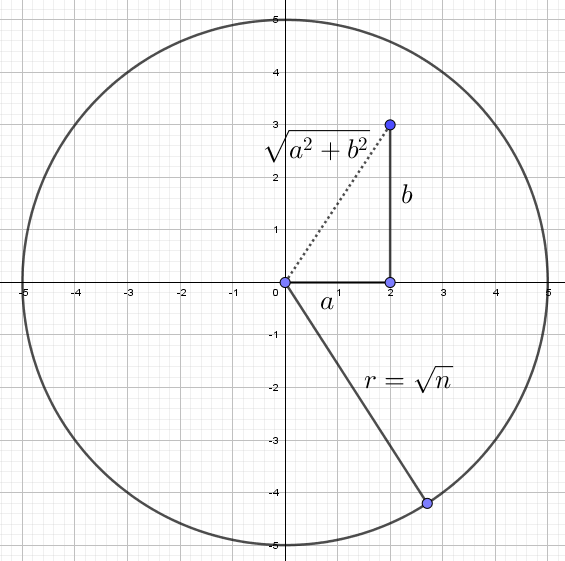
\includegraphics[height=7cm]{abszampar1.png}
			\caption{Pontok a körön belül}\label{abszampar1}
		\end{figure}
	
		Ezeket a kör belsejébe eső egész koordinátájú pontokat szokás rácspontoknak is nevezni. Hogyan tudnánk megbecsülni adott $n$ mellett a $\sqrt{n}$ sugarú kör belsejébe eső rácspontok számát? Tegyünk minden rácspontba egy egységoldalú négyzetet úgy, hogy a négyzet bal felső sarka legyen a rácspont:
		
		\begin{figure}[h] %h=here, t=top, b=bottom
			\centering
			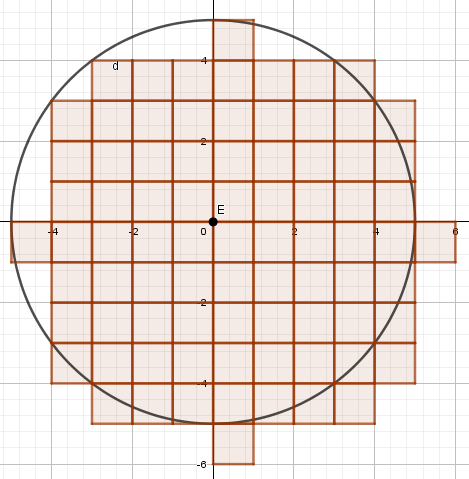
\includegraphics[height=8cm]{abszampar2.png}
			\caption{Négyzetek}\label{abszampar2}
		\end{figure}
		
		Ha ezen négyzetek területét becsüljük meg, ugyanazt a számot kapjuk, mintha a pontok számát becsülnénk. Látjuk, hogy a négyzetek ,,körülbelül kitöltik'' a kört. Az a baj, hogy bizonyos pontok kilógnak, bizonyos pontjait pedig nem fedik le.
		
		Vegyünk egy olyan kört, aminek sugara $\sqrt{n}-\sqrt{2}$ és egy olyat, melynek $\sqrt{n}+\sqrt{2}$.
		
		\begin{figure}[h] %h=here, t=top, b=bottom
			\centering
			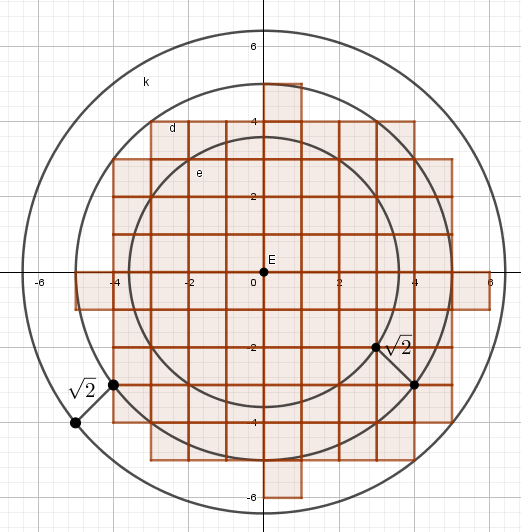
\includegraphics[height=8cm]{abszampar3.png}
			\caption{Új körök}\label{abszampar3}
		\end{figure}
		
		Mivel az egységoldalú négyzet két legtávolabbi pontja $\sqrt{2}$, így a kisebb körnek minden egyes pontját fedi valamely pontja valamely négyzetnek. Tehát a kisebb kör területe jó alsó becslés a négyzetek területére (azaz a pontok számára). Hasonlóan a külső kör területe jó felső becslés, tehát:
		\[ (\sqrt{n}-\sqrt{2})^2\cdot \pi  \leq  T\leq  (\sqrt{n}+\sqrt{2})^2\cdot \pi  \]
		osztva $n$-nel:
		\[ \dfrac{(\sqrt{n}-\sqrt{2})^2\cdot \pi}{n} \leq A_n \leq  \dfrac{(\sqrt{n}+\sqrt{2})^2\cdot \pi}{n} \]
		Közrefogtuk $A_n$ sorozatot két olyan sorozattal, melyek mindegyike $\pi$-hez tart (például):
		\[ \lim\limits_{n\to\infty} \dfrac{(\sqrt{n}-\sqrt{2})^2\cdot \pi}{n} = \lim\limits_{n\to\infty} \dfrac{(n-2\sqrt{2n}+2)\cdot \pi}{n} = \pi\cdot  \lim\limits_{n\to\infty} \left( \dfrac{n}{n} -2 \sqrt{\dfrac{2n}{n^2}} + \dfrac{2}{n} \right) = \pi \cdot (1-0+0) = \pi  \]
		Így tehát a rendőr-elv miatt $\lim\limits_{n\to \infty} A_n = \pi$.
	\end{proof}


	\chapter{Fermat, Wiles, Rivest, Shamir, Adlemann}
	
	A 8. és 10. előadásról egyelőre csak a fontosabb tételeket írom fel, bizonyításukra igyekszem későbbiekben sort keríteni (amennyiben időm engedi és megfejtem a füzetemben lévő hieroglifákat).
	
	\section{Pitagoraszi számhármasok (emlék)}
	
	\begin{lem}[Szorzat-hatvány lemma]\label{szhl}
		Legyen $R$ egy alaptételes gyűrű. Amennyiben $a,b\in R$, $(a,b)=1$ és $\exists x\in R, n\in \Z$ melyre $a\cdot b = x^n$ akkor $\exists u,v\in R$ melyekre $a = \varepsilon u^n$ és $b = \varepsilon v^n$ ahol $\varepsilon$ az $R$ gyűrű (egyik) egysége.
	\end{lem}

	Röviden, a lényeget kiemelve, de pontatlanul leírva:
	\[ (a,b)=1 \hspace{5mm} \text{és} \hspace{5mm} a\cdot b = x^n \hspace{10mm} \Rightarrow \hspace{10mm} a = u^n \hspace{5mm} \text{és} \hspace{5mm} b = v^n  \]
	
	\begin{mj}
		Kellenek az egységszeresek, hiszen $R=\Z$ esetén $a=-1$, $b=-1$ és $n=2$ szereposztással $\exists x\in \Z$, melyre $a\cdot b = (-1)\cdot (-1) = x^2$, ilyen például az $x=1$. De az nem igaz, hogy $\exists u,v\in \Z$, melyekre $a=-1=u^2$ és $b=-1=v^2$.
	\end{mj}
	
	\begin{theo}
		Az $x^2+y^2=z^2$ egyenlet alapmegoldásai (melyekre $(x,y,z)=1$):
		\[ x=2\cdot r \cdot s \hspace{10mm} \text{és} \hspace{10mm} y=r^2-s^2 \hspace{10mm} \text{és} \hspace{10mm} z = r^2 + s^2 \]
		ahol $(r,s)=1$ és $r\not \equiv s\ (2)$.
	\end{theo}
	
	\section{Fermat-sejtés, Wiles-tétel}
	
	\begin{theo}[Fermat-sejtés, Wiles-tétel]
		Az $x^n+y^n=z^n$ egyenlet $n\geq3$ esetén nem oldható meg a pozitív egész számok körében.
	\end{theo}

	\begin{theo}
		Az $x^4+y^4=z^2$ egyenlet nem oldható meg a pozitív egész számok körében.
	\end{theo}
	
	\section{Titkosírás (RSA)}
	
	\chapter{Egészen új egészek}
	\section{Gauss-egészek}
	
	\begin{defi}
		Azokat az komplex számokat, melyek valós és képzetes része is egész, \textbf{Gauss-egész}eknek nevezzük. A Gauss-egészek halmazát jelöli\footnote{sok helyen $\Z[i]$ jelöléssel is találkozhatunk} $\mathcal{G}=\{ a+bi\in C \mid a,b\in \Z  \}$
	\end{defi}

	A Gauss-egészeket gyakran görög abc betűivel fogjuk jelölni.
	
	Algebra2-ből a komplex számoknak láttuk egy geometriai átfogalmazását, bevezettük a komplex számsíkot. Sokszor hasznos úgy gondolkodnunk, hogy a Gauss-egészek a komplex számsík rácspontjainak felelnek meg.

	\begin{theo}
		A Gauss-egészek gyűrűt alkotnak a szokásos komplex számokra definiált összeadásra és szorzásra: $(\mathcal{G},+,\cdot)$ gyűrű.
	\end{theo}

	\begin{proof}
		Mivel $\mathcal{G}\subseteq \C$, ezért csak azt kell belátnunk, hogy zárt az összeadásra és szorzásra, van nullelem és ellentett.
		\begin{itemize}
			\item{Összeadásra zártság: adott $\alpha=a+bi\in \mathcal{G}$ és $\beta=c+di\in \mathcal{G}$, kellene: $\alpha+\beta\in\mathcal{G}$. Ez nyilván teljesül, hiszen $\alpha+\beta = (a+c) + (b+d)i$ ahol $a+c\in \Z$ és $b+d\in \Z$ tehát $\alpha+\beta\in \mathcal{G}$ }
			\item{Szorzásra zártság: adott $\alpha=a+bi\in \mathcal{G}$ és $\beta=c+di\in \mathcal{G}$, kellene: $\alpha \cdot \beta\in\mathcal{G}$. Ez nyilván teljesül, hiszen $\alpha \cdot \beta = (ac-bd) + (ad+bc)i$ ahol $ac-bd\in \Z$ és $ad+bc\in \Z$ tehát $\alpha \cdot \beta\in \mathcal{G}$ }
			\item{Van nullelem: $0=0+0\cdot i \in \mathcal{G}$}
			\item{Van ellentett: Adott $a+bi\in \mathcal{G}$ esetén $-a-bi\in \mathcal{G}$ teljesül.}
		\end{itemize}
	\end{proof}

	Sőt ennél többet is látunk, $\mathcal{G}$ egy szokásos gyűrű. A szorzás kommutatív, nullosztómentes (hiszen ha lennének nullosztók, akkor a komplex számok testében is, ami nyilán nem lehet) és egységelemes, hiszen $1=1+0\cdot i\in \mathcal{G}$.
	
	\textbf{Emlék:} Szokásos gyűrűkre vezettünk be számelméleti fogalmakat és azt is láttuk (\ref{szatbiz}. tétel), hogy ha egy gyűrű euklideszi, akkor alaptételes is (teljesül benne a számelmélet alaptétele). Jó lenne, ha be tudnánk látni, hogy $\mathcal{G}$ euklideszi.
	
	\textbf{Emlék:} Komplex számok normájáról beláttuk (Algebra2), hogy szorzat normája a normák szorzata ($N(\alpha\cdot \beta) = N(\alpha)\cdot N(\beta)$) és csakis a $0$ komplex szám normája $0$: $N(\alpha) = 0 \Leftrightarrow \alpha = 0$.

	\begin{theo}
		A Gauss-egészek gyűrűje euklideszi.
	\end{theo}
	
	\begin{proof}
		Azt kellene belátnunk, hogy létezik ,,maradékos osztás'', vagyis a \ref{euklgy}. definíció szerint keresünk egy $\varphi\colon \G\setminus \{0\} \to \Z^{+}$ leképezést, melyre $\forall \alpha, \beta\in \G\setminus \{0\}$ esetén $\exists \gamma,\delta\in \G$ melyre
		\begin{center}
			$\alpha =\beta \cdot \gamma  +\delta$ \hspace{1cm} és \hspace{1cm} $\varphi(\delta)<\varphi(\beta)$ \hspace{0.25cm} vagy \hspace{0.25cm} $\delta=0$
		\end{center}
		A norma éppenséggel nekünk egy jó $\varphi$ leképezés lesz most. Az értelmezett $0$ komplex számra is, de ez most nekünk nem baj, sőt előnyünkre is válik, mert nem kell a $\delta = 0$ esettel foglalkoznunk, hiszen akkor $N(\delta)= 0$, tehát $N(\delta)=0<N(\beta)$ automatikusan teljesül, hiszen $N(\beta)\neq 0$, mert csak a $0$ szám normája lehet $0$.
		
		Hasznos továbbá ha Gauss-egészek helyett komplex számokban gondolkozunk és úgy fogalmazzuk át milyen $\gamma$ és $\delta$ megtalálása a célunk. Komplex számokba átlépve a $\beta\neq 0$, tehát van neki inverze, oszthatunk vele:
		\begin{center}
			$\dfrac{\alpha}{\beta} = \gamma  +\dfrac{\delta}{\beta}$ \hspace{1cm} és \hspace{1cm} $N(\delta)<N(\beta) \hspace{0.2cm} \Leftrightarrow \hspace{0.2cm} N\left (\dfrac{\delta}{\beta}\right)<1$
		\end{center}
		Az $\alpha$ és $\beta$ adottak, tehát ki tudjuk számolni a hányadosukat, legyen ez $z=\dfrac{\alpha}{\beta}\in\C$ komplex szám a komplex síkon. Találnunk kell olyan $\gamma\in \G$ Gauss-egészt, azaz rácspontot, melytől a $z$ eltérése ,,kisebb'' mint 1.
		
		Ez az idézőjel azért van itt, mert komplex számokra nincs rendezésünk, de a norma már valós, arra van, tehát:
		\[ z - \gamma = \dfrac{\delta}{\beta} \hspace{0.2cm} \Rightarrow \hspace{0.2cm} N(z-\gamma) = N\left(\dfrac{\delta}{\beta}\right) < 1  \]
		Hogyan állítsunk elő ilyen $\gamma$ Gauss-egészt? Keressük először is meg a $z$ komplex számot a komplex síkon. Mondjuk megtaláltuk itt:
		
		\[ 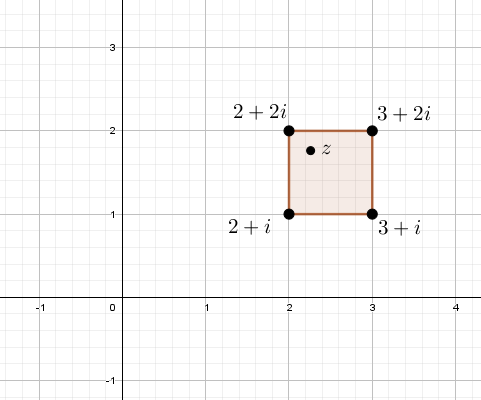
\includegraphics[height=5cm]{eukl1.png} \]
		
		Innentől kezdve csak azzal az egységoldalú négyzettel fogunk foglalkozni, mely tartalmazza $z$-t és csúcsai rácspontok (ilyen nem feltétlenül 1 van, lehet 4 is, de akkor válasszunk egyet):
		
		\[ 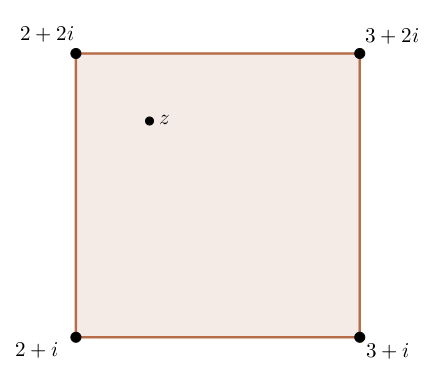
\includegraphics[height=7cm]{eukl2.png} \]
	
		Elég volna megmutatnunk, hogy ennek a négyzetnek van olyan csúcsa, melytől $z$ távolsága legfeljebb $1$, az általa reprezentált Gauss-egész jó lesz $\gamma$ választásnak, továbbá $\delta = \alpha - \beta \cdot \gamma$ választással $\delta$ is meglenne.
		
		Nézzük meg mik azok a pontok, amelyek az egyes csúcsoktól legfeljebb $1$ távolságra vannak, vagyis mely pontokhoz lennének jó választások az egyes csúcsok:
		
		\begin{center}
			\begin{tabular}{c c c}
				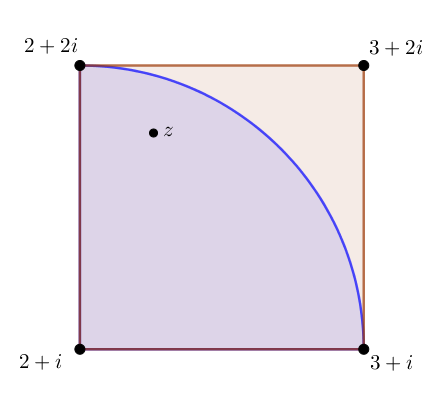
\includegraphics[height=4cm]{eukl3.png}
				&
				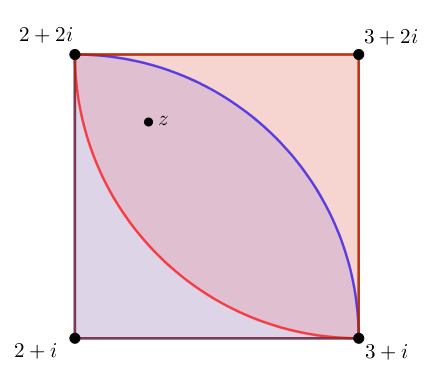
\includegraphics[height=4cm]{eukl4.png}
				&
				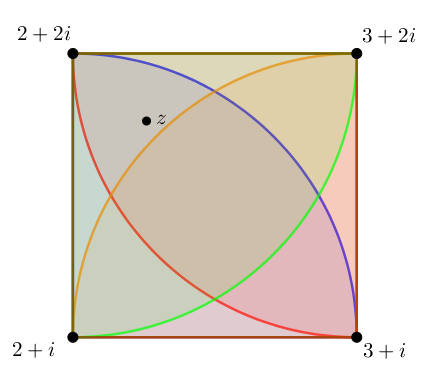
\includegraphics[height=4cm]{eukl5.png} \\
			\end{tabular}
		\end{center}
		Látjuk, hogy már a bal alsó rácspont is jó választás lenne most számunkra, de általánosságban kell gondolkoznunk.
		
		A bal alsó és a jobb felső rácspont valamelyike általánosságban is minden $z$ esetén jó választás, ahogy az ábrán látható: nincs olyan pontja az egységnégyzetnek, mely távolsága mindkettőtől $1$-nél több volna.
		
		Bár a második kép is tanulságos olyan szempontból, hogy van ami kétszer is fedésbe került (tehát több jó rácspont is választható hozzá), a harmadik képen látszik igazán, hogy minden pont esetén legalább $2$ rácspont választható volna, tehát ez a bizonyos ,,maradékos osztás'' nem egyértelmű! (Nem is volt célunk, hogy az legyen, csak megmutatni, hogy van).
	\end{proof}

	Innen tehát automatikusan következik, hogy teljesül a számelmélet alaptétele $\G$-ben. Ezért jó az euklideszi tulajdonsága egy gyűrűnek. Hamarabb beláttuk a SZAT-ot, minthogy megvizsgáltuk volna az egységeket vagy prímeket a gyűrűben. Kerítsünk azért erre is sort.
	
	\begin{lem}\label{normoszt}
		Minden Gauss-egész osztja a normáját: $\forall \alpha \in \G$-re: $\alpha \mid N(\alpha)$
	\end{lem}

	\begin{proof}
		Azt kell belátnunk, hogy $\exists \beta \in \G$, melyre $\alpha \cdot \beta = N(\alpha)$.
		
		Tudjuk, hogy $N(\alpha)= \alpha\cdot \overline{\alpha}$, és ha $\alpha=a+bi$ Gauss-egész, akkor $\overline{\alpha}=a-bi$ is Gauss-egész. Így $\beta = \overline{\alpha}$ választással máris látjuk, hogy $\alpha\mid N(\alpha)$.
	\end{proof}

	\begin{lem}\label{normakoszt}
		Legyenek $\alpha,\beta\in \G$ és $\alpha \mid \beta$. Ekkor $N(\alpha)\mid N(\beta)$ is teljesül.
	\end{lem}
	
	\begin{proof}
		A feltétel szerint $\exists \gamma\in \G$, melyre $\beta = \alpha \cdot \gamma$. Ekkor mindkét oldal normáját véve
		\[ N(\beta) = N(\alpha\cdot \gamma) = N(\alpha)\cdot N(\gamma) \]
		ami éppen azt jelenti, hogy $N(\alpha)\mid N(\beta)$.
	\end{proof}
	
	\begin{theo}
		A Gauss-egészek között $4$ egység létezik, ezek: $1,-1,i,-i$.
	\end{theo} 

	\begin{proof}
		Egységek azok, amelyek osztják a gyűrű egységelemét, tehát az $1$-et: $\varepsilon\mid 1$. A \ref{normakoszt}. lemma alapján ekkor $N(\varepsilon)\mid N(1)=1$.
		
		Amennyiben $\varepsilon=a+bi$ alakú, akkor $N(\varepsilon)=a^2+b^2$. Mivel egész számok körében az $1$-nek csak $2$ osztója van, ezért $2$ lehetséges esetünk van:
		\[ a^2+b^2 = 1 \hspace{3mm} \text{vagy} \hspace{3mm} a^2+b^2=-1  \]
		Utóbbi nyilvánvalóan nem lehetséges, mert baloldalon nemnegatív, jobboldalon pedig negatív szám áll. Mi a helyzet az elsővel? Hányféleképpen áll elő az $1$ két négyzetszám összegeként? Négyféleképpen:
		\[ 1=1^2+0^2 \hspace{3mm} \text{vagy} \hspace{3mm} 1=(-1)^2+0^2 \hspace{3mm} \text{vagy} \hspace{3mm} 1=0^2+1^2 \hspace{3mm} \text{vagy} \hspace{3mm} 1=0^2+(-1)^2 \]
		az egyes esetekben az $\varepsilon$ komplex szám értéke:
		\[ \varepsilon=1+0\cdot i=1 \hspace{3mm} \text{vagy} \hspace{3mm} \varepsilon=-1+0\cdot i=-1 \hspace{3mm} \text{vagy} \hspace{3mm} \varepsilon=0+1\cdot i=i \hspace{3mm} \text{vagy} \hspace{3mm} \varepsilon=0-1\cdot i = -i \]
	\end{proof}

	Tehát itt pontosan $4$ egységünk van, úgy is mondhatnám a Gauss-egészek között $4$-féle ,,előjele'' létezik minden számnak.
	
	\begin{mj}
		Vannak olyan alaptételes gyűrűk is, amelyekben végtelen sok egység van. Ilyen például $\{a+b\cdot\sqrt{2} \mid a,b\in \Z \}$. Itt egység a $\sqrt{2}+1$, hiszen
		\[ (\sqrt{2}-1)\cdot(\sqrt{2}+1) = 1 \hspace{3mm} \Rightarrow \hspace{3mm} \sqrt{2}+1\mid 1  \]
		De ha valami egység, akkor annak négyzete, sőt akárhanyadik hatványa is, tehát $(\sqrt{2}+1)^n$ mindannyian egységek és különböző $n$-ek esetén különböző számok az exponenciális függvény szigorú monotonitása miatt. Tehát itt máris mutattunk végtelen sok egységet.
	\end{mj}
	
	\section{Gauss-prímek}

	Ebben a fejezetben arra a kérdésre keressük a választ, hogy melyek a Gauss-prímek $\G$-ben. Ehhez jó néhány segédállításra szükségünk lesz. Jelzem, hogy ebben a fejezetben inkább a Freud: Számelmélet könyv szerint haladok, az alapján nekem könnyebb volt megérteni ezt a témakört.

	A Gauss-prímeket általában $\pi$ görög betűvel fogom jelölni.

	\begin{lem}\label{prnorm}
		Egy $\pi\in \G$ Gauss-prím normája legalább $2$: $N(\pi)\geq 2$
	\end{lem}

	\begin{proof}
		Legyen $\pi = a + bi$, ekkor azt kellene igazolnunk, hogy $N(\pi)=a^2+b^2\geq 2$. Tudjuk, hogy bármely komplex szám normája nemnegatív, tehát ha ez nem lenne igaz, akkor $a^2+b^2 = 0$ vagy $a^2+b^2=1$ lehetne. Mindkettő ellentmondás, mert első esetben $\pi = 0$, ami nem prím, másik esetben pedig $\pi$ egység volna, ami szintén nem lehet prím (a prímtulajdonság definíciója úgy kezdődik, hogy olyan egységtől különböző szám, melyre...).
	\end{proof}

	%L: p-nek osztója
	
	\begin{lem}\label{gpl1}
		Amennyiben $\pi\in \G$ prím, akkor $\exists p\in \Z$, melyre $\pi \mid p$.
	\end{lem}

	\begin{proof}
		A \ref{normoszt}. lemma alapján $\pi \mid N(\pi)$. Mivel $\pi$ prím \ref{prnorm}. lemma miatt $N(\pi)\geq 2$, tehát nem $0$ és nem egység. Ekkor a $\Z$-ben teljesülő számelmélet alaptétele miatt van neki prímtényezős felbontása:
		\[ N(\pi) = p_1^{\alpha_1} \cdot \ldots \cdot p_n^{\alpha_n}  \]
		tehát visszatérve a Gauss-egészek körébe $\pi \mid p_1^{\alpha_1} \cdot \ldots \cdot p_n^{\alpha_n} $
		használva $\pi$ prímtulajdonságát ha egy szorzatot oszt, akkor annak valamely tényezőjét is, tehát $\exists p$ prím, melyre $\pi \mid p$. Ezt kellett igazolni.
	\end{proof}
	
	Ez jó hír, ezek szerint úgy érdemes keresnünk a Gauss-prímeket, hogy a szokásos egész prímeink osztóit vizsgáljuk. Látni fogjuk, hogy megint érdemes különvenni a $2$-t, a $4k-1$ alakú, és a $4k+1$ alakú prímeket. Lesz ezek közül amelyik megmarad Gauss-prímnek is, de olyan is ami felbomlik. Hasznos észrevétel, hogy igencsak korlátozottan tudnak a prímeink felbomlani Gauss-prímek szorzatára, legfeljebb $2$-re.
	
	\begin{lem}\label{gpl2}
		Minden $p$ pozitív prímszám vagy maga is Gauss-prím, vagy pedig pontosan két Gauss-prímnek a szorzata, amelyek normája $p$ és amelyek egymás konjugáltjai.\footnote{Freud: Számelmélet, 7.4.14. Tétel (ii)}
	\end{lem}

	\begin{proof}
		Azt kell belátnunk, hogy ha $p$ nem Gauss-prím, akkor ő pontosan $2$ Gauss-prím szorzata.
		
		Mivel $p$ nem Gauss-prím, a számelmélet alaptétele szerint $\G$-ben $p$ felbomlik legalább $2$ Gauss-prím szorzatára: $\exists \pi_1,\pi_2,\ldots,\pi_r$
		\[ p = \pi_1 \cdot \pi_2 \cdot \ldots \cdot \pi_r  \]
		Mindkét oldal normáját véve:
		\[ p^2=N(p) = N(\pi_1 \cdot \pi_2 \cdot \ldots \cdot \pi_r) = N(\pi_1) \cdot N(\pi_2)\cdot \ldots \cdot N(\pi_r) \]
		Mivel itt minden $\pi_i$ Gauss-prím, ezért \ref{prnorm}. lemma szerint $N(\pi_i)\geq 2$, tehát a jobboldali szorzat egyik tényezője sem egység.
		
		Viszont $p^2$ csakis úgy bontható legalább $2$ szám szorzatára (melyek egyike sem egység), hogy $p^2 = p\cdot p$. Tehát azt kaptuk, hogy jobboldalon pontosan $2$ szám áll, azaz $p=\pi_1\cdot \pi_2$.
		
		De azt is tudjuk, hogy mindkét Gauss-prím normája $p$ kell legyen, tehát speciálisan az elsőé is $p = N(\pi_1) = \pi_1 \cdot \overline{\pi_1} $. Tehát valóban $p$ két olyan Gauss-prím szorzataként áll elő, melyek egymás konjugáltjai.
	\end{proof}

	\begin{theo}
		A $2$ kanonikus alakja $2=(-i)\cdot (1+i)^2$
	\end{theo}

	\begin{proof}
		A $2$ felbontható $2$ Gauss-prím szorzatára, így ő nem Gauss-prím: $2=(1+i)\cdot (1-i)$.
		A \ref{gpl2}. lemma alapján mivel $2$ nem Gauss-prím, ezért pontosan $2$ Gauss-prím szorzataként áll elő, melyek egymás konjugáltjai: $1+i$ és $1-i$. De vigyázat! Ez nem $2$ különböző Gauss-prím, ez csak $1$, hiszen $1-i = (-i) \cdot (1+i)$, tehát ezek egységszeresei egymásnak.
		
		Vagyis a $2$-nek egységszerestől eltekintve egyetlen prímosztója van, az $1+i$, melynek négyzetével is osztható. Mivel a $2$ csupán egységszerese $(1+i)^2$-nek, ezért a $2$ kanonikus alakja 
		\[ 2 = \varepsilon \cdot \pi_1^{\alpha_1} \cdot \ldots \cdot \pi_r^{\alpha_r} =  (-i)\cdot (1+i)^2 \]
	\end{proof}

	\begin{theo}
		A $p=4k-1$ alakú prímek Gauss-prímek is.
	\end{theo}

	\begin{proof}
		Indirekt tegyük fel, hogy egy $p=4k-1$ alakú prím nem Gauss-prím. Ekkor a \ref{gpl2}. lemma szerint $2$ olyan Gauss-prím szorzata, melyek normája $p$. Tehát van olyan Gauss-prím, legyen ez most $\pi = a+bi$, melynek normája: $N(\pi)= a^2 + b^2 = p$. De ez ellentmond a két-négyzetszám tételnek (\ref{knszt}. tétel), hiszen $p$ kanonikus alakjában (ami $p = p^1$) szerepel egy $4k-1$ alakú prím páratlan hatványon.
	\end{proof}
	
	\begin{theo}\label{4kp1}
		A $p=4k+1$ alakú prímek nem Gauss-prímek, egységszerestől eltekintve egyértelműen felbomlanak $2$ Gauss-prím szorzatára, melyek egymás konjugáltjai, de nem egymás egységszeresei.
	\end{theo}

	\begin{proof}
		Itt jó néhány dolgot be kell látnunk, haladjunk lépésekben.
		
		\textit{Nem prímek:}
		
		Indirekt tegyük fel, hogy $p=4k+1$ Gauss-prím. Ekkor \ref{wilson_kov}. lemma szerint $x^2\equiv -1\ (p)$ kongruencia megoldható, vagyis $\exists x$ melyre $p\mid x^2+1 = (x+i)\cdot (x-i)$. Feltettük, hogy $p$ Gauss-prím és egy prím ha oszt egy szorzatot, akkor valamelyik tényezőt is, azaz
		\[ p\mid x+i  \hspace{10mm} \text{vagy} \hspace{10mm} p\mid x-i \]
		Az oszthatóság definíciója szerint $\exists \alpha = a+bi \in \G$, Gauss-egész, melyre
		\[ p\cdot (a+bi) = x+i  \hspace{10mm} \text{vagy} \hspace{10mm} p\cdot (a+bi) = x-i \]
		beszorozva
		\[ p\cdot a+\color{red} p\cdot b\color{black} \cdot i = x+\color{red} 1\color{black}\cdot i  \hspace{10mm} \text{vagy} \hspace{10mm} p\cdot a + \color{blue} p\cdot b \color{black} \cdot i = x+\color{blue} (-1) \color{black} \cdot i \]
		komplex számok egyenlősége esetén a képzetes részük is megegyezik (ami jelen esetben egész)
		\[ p\cdot b = 1 \hspace{10mm} \text{vagy} \hspace{10mm} p\cdot b = -1 \]
		ami ellentmondás, mert sem az $1$-nek, sem a $-1$-nek nem lehet osztója egy $p$ prímszám.
		
		\textit{Egyértelműen felbomlanak:}
		
		Azt már nem kell igazolni, hogy felbomlanak pontosan $2$ Gauss-prím szorzatára, melyek normája $p$ és egymás konjugáltjai, hiszen \ref{gpl2}. lemma szerint ez minden $p\in \Z$ prímre teljesül ami nem Gauss-prím.
		
		Az egyértelműség rész van hátra. Tegyük fel, hogy többféleképpen is felbomlik:
		\[ p=\pi_1\cdot \overline{\pi_1} = \pi_2 \cdot \overline{\pi_2} \]
		ahol $p=N(\pi_1) = N(\overline{\pi_1})=N(\pi_2) = N(\overline{\pi_2})$. Ekkor $\pi_2 \mid \pi_1\cdot \overline{\pi_1}$, tehát a prímtulajdonság miatt a szorzat egyik tényezőjét is osztja:
		\[ \pi_2 \mid \pi_1 \hspace{10mm} \text{vagy} \hspace{10mm} \pi_2\mid \overline{\pi_1}  \]
		Belátható, hogy első esetben $\pi_2 = \varepsilon \cdot \pi_1$, másodikban $\pi_2 = \varepsilon \cdot \overline{\pi_1}$. Mindkét esetben azt használjuk ki, hogy normájuk megegyezik. Például az első esetet én úgy csinálnám, hogy
		\[ \pi_2 \mid \pi_1 \hspace{5mm} \Rightarrow \hspace{5mm} \exists \gamma\colon \gamma\cdot \pi_2 = \pi_1  \]
		Mindkét oldal normáját véve
		\[ N(\gamma\cdot \pi_2) = N(\gamma) \cdot N(\pi_2) = N(\pi_1) \]
		használva, hogy $N(\pi_1)=N(\pi_2)=p$
		\[ N(\gamma)\cdot p = p \hspace{5mm} \Rightarrow \hspace{5mm} N(\gamma) = 1 \]
		vagyis $\gamma = \varepsilon$ egység.
		
		\textit{Nem egymás egységszeresei:}
		
		Itt csak végig kell próbálgatni, hogy mikor lehet egy Gauss-egész és konjugáltja egymás egységszerese. Meg kell nézni, hogyha az egyiket megszorzom egy egységgel, mikor kaphatom a másikat. A $4$ egység szerint nézzük meg a $4$ esetet: $\alpha = a+bi, \overline{\alpha} = a-bi, \varepsilon$ egység, milyen feltétel esetén lesz $\varepsilon \cdot \alpha = \overline{\alpha}$? (Tudjuk azt is, hogy $N(\alpha)=p$ prímszám.)
		\begin{itemize}
			\item{$\varepsilon = 1$ esetén:
			\[ 1\cdot (a+bi) = a-bi \hspace{5mm} \Rightarrow \hspace{5mm} a=a \hspace{5mm} \text{és} \hspace{5mm} b=-b \hspace{5mm} \Rightarrow \hspace{5mm} \alpha = a \] vagyis $N(\alpha)= N(a) = a^2\neq p$ prímszám.
			}
			\item{$\varepsilon = -1$ esetén:
			\[ -1\cdot (a+bi) = a-bi \hspace{5mm} \Rightarrow \hspace{5mm} -a=a \hspace{5mm} \text{és} \hspace{5mm} -b=-b \hspace{5mm} \Rightarrow \hspace{5mm} \alpha = b\cdot i \]
			vagyis $N(\alpha)= N(b\cdot i) = b^2\neq p$ prímszám.
			}
			\item{$\varepsilon = i$ esetén:
			\[ i\cdot (a+bi) = a-bi \hspace{5mm} \Rightarrow \hspace{5mm} -b=a \hspace{5mm} \text{és} \hspace{5mm} a=-b \hspace{5mm} \Rightarrow \hspace{5mm} \alpha = a-ai \] vagyis $N(\alpha)= N(a-ai) = 2\cdot a^2\neq p = 4k+1$ alakú prímszám.
			}
			\item{$\varepsilon = -i$ esetén:
				\[ -i\cdot (a+bi) = a-bi \hspace{5mm} \Rightarrow \hspace{5mm} b=a \hspace{5mm} \text{és} \hspace{5mm} -a=-b \hspace{5mm} \Rightarrow \hspace{5mm} \alpha = a+ai \] vagyis $N(\alpha)= N(a+ai) = 2\cdot a^2\neq p = 4k+1$ alakú prímszám.
			}
		\end{itemize}
		
	\end{proof}
	
	Ezzel az előbbi tétellel egyben törlesztettük egy régi adósságunkat is, a két-négyzetszám tétellel kapcsolatban.
	
	\begin{theo}\label{torlesztes}
		Minden $4k+1$ alakú prímszám 
		előáll $2$ négyzetszám összegeként.
	\end{theo}

	\begin{proof}
		Az előző, \ref{4kp1}. tétel szerint minden $p=4k+1$ alakú prímszámhoz egyértelműen léteznek $\pi_1,\pi_2$ Gauss-prímek, melyekre $p=\pi_1\cdot \pi_2$ és ezek egymás konjugáltjai, valamint mindkettő normája $N(\pi_1)=N(\pi_2)=a^2+b^2=p$.
	\end{proof}

	\begin{mj}
		Ezzel nem csak azt láttuk be, hogy minden $p=4k+1$ alakú prímszám előáll két négyzetszám összegeként, de ráadásul ez az előállítás $a$ és $b$ sorrendjétől és egységszeresektől eltekintve egyértelmű. 
	\end{mj}

	\textbf{Összefoglalva: }A Gauss-prímek tehát a következők (és ezek egységszereseik):
	\begin{itemize}
		\item{$1+i$}
		\item{$p$, ahol $p=4k-1\in \Z$ prím}
		\item{$\pi$ és $\overline{\pi}$, ahol $\pi\cdot \overline{\pi}=p=4k+1\in \Z$ prímszám}
	\end{itemize}
	
	\begin{pl}
		Adjuk meg a prímtényezős felbontását az $5$ és a $78+702 i$ Gauss-egészeknek!
		
		\begin{enumerate}[label = (\alph*)]
			\item{Az $5$ egy $4k+1$ alakú prím, tehát egyetlen dolgunk, hogy felírjuk két-négyzetszám összegeként:
			\[ 5 = 1+4 = 1^2+4^2 = (1+2i)\cdot (1-2i)  \]	
			Tudjuk, hogy a $4k+1$ alakú prímek $2$ olyan Gauss-prímre bomlanak fel, melyek egymás konjugáltjai, de nem egységszeresei, tehát az $5$-nek ez a két prímosztója van, vagyis az $5$ kanonikus alakja $5=(1+2i)^1\cdot (1-2i)^1$.
		}
		\item{Most picit hosszadalmasabb dolgunk lesz, de mindenekelőtt bontsuk fel a valós és a képzetes részt prímtényezőkre és emeljük ki a legnagyobb közös osztót:
		\[ 78+702 i = (2\cdot 3\cdot 13) + (2\cdot 3^3\cdot 13) i \]
		Kiemelhető a $2\cdot 3\cdot 13$ legnagyobb közös osztó:
		\[ 78 + 702 i = (2\cdot 3\cdot 13) \cdot (1+9i) \]
		Innentől külön dolgozhatunk a $2\cdot 3\cdot 13$-mal és az $1+9i$-vel.
		
		A $2\cdot 3\cdot 13$ esete könnyű lesz, hiszen a $2$ felbontását tudjuk, hogy $2=(-i)\cdot (1+i)^2$, a $3=4k-1$ alakú prím, tehát ő egyben Gauss-prím is, a $13$ esete pedig az előző feladat $5$ esetéhez hasonló, hiszen ez is $4k+1$ alakú prím:
		\[ 13 = 9+4 = 3^2+2^2 = (3+2i)\cdot (3-2i)  \]
		Tehát a feladat ,,felével'' megvagyunk: $2\cdot 3\cdot 13 = (-i)\cdot 3\cdot (1+i)^2\cdot (3+2i)^1\cdot (3-2i)^1$
		
		Mit kezdjünk az $1+9i$-vel? A szokásos trükk, hogy láttuk a \ref{normoszt}. lemmában, hogy minden Gauss-egész osztja a normáját, tehát
		\[ 1+9i \mid N(1+9i) = 1^2+9^2 = 1+81 = 82 = 2\cdot 41  \]
		Bontsuk a normáját Gauss-prímek szorzatára, hiszen $1+9i$ osztói csakis normájának osztói közül kerülhetnek ki ($41 = 25+16$):
		\[ 1+9i \mid (-i)\cdot (1+i)^2\cdot (5+4i)\cdot (5-4i)  \]
		Nézzük meg innen melyik szám osztja $1+9i$-t. Ezt egyszerűen úgy nézzük meg, hogy elosztjuk vele, és az eredményről eldöntjük, hogy Gauss-egész lesz-e: próbáljuk először elosztani $1+i$-vel\footnote{osztásnál a szokásos módon konjugálttal célszerű bővíteni}:
		\[ \dfrac{1+9i}{1+i} = \dfrac{1+9i}{1+i} \cdot \dfrac{1-i}{1-i} = \dfrac{(1+9i)\cdot(1-i)}{(1+i)\cdot (1-i)} = \dfrac{10+8i}{2} = 5+4i   \]
		tehát
		\[ 1+9i = (1+i)\cdot (5+4i)  \]
		
		A keresett szám prímfelbontása:
		\[ 78+702i = (-i)\cdot 3 \cdot (1+i)^3 \cdot (3+2i)^1\cdot (3-2i)^1\cdot (5+4i)^1  \]
		
		}
		\end{enumerate}
	\end{pl}

	\section{Alkalmazások}
	
	%40:00
	
	Ebben a fejezetben két ,,régi'' tételt fogunk Gauss-egészekkel újra bebizonyítani, első a két-négyzetszám tétel egyik fele lesz, másik a Pitagoraszi számhármasok kinézete.
	
	\begin{theo}[Két-négyzetszám tétel]
		Legyen $n$ egész kanonikus alakja
		\[  n = 2^{\alpha} \cdot \prod p_i^{\alpha_i} \cdot \prod q_i^{\beta_i} \]
		ahol $\forall p_i=4k+1$ és $\forall q_j = 4k-1$ alakú prím. Ha az $n$ szám előáll két négyzetszám összegeként, akkor $\forall \beta_j$ páros.
	\end{theo}

	\begin{proof}
		Tegyük fel, hogy $n=x^2+y^2=(x+yi)\cdot(x-yi)$. Bontsuk fel az utóbbi szorzat mindkét tényezőjét Gauss-prímek szorzatára. Milyen Gauss-prímeket ismerünk? Van az $1+i$, vannak a $q_i=4k-1\in \Z$ egész prímek és az olyan $\pi_i$ egyéb Gauss-prímek, melyek konjugáltja is prím és melyekre $\pi_i\cdot \overline{\pi_i} = N(\pi_i) = p_i = 4k+1\in \Z$ egész prím.
		
		A Gauss-egész prímfelbontásában tegyünk különbséget köztük és az előbbi jelölésekkel akkor általánosságban az $x+yi$ Gauss-egész kanonikus alakja:
		\[ x+yi = (1+i)^b\cdot \prod \pi_i^{c_i} \cdot \prod \overline{\pi_i}^{d_i}\cdot \prod q_i^{\gamma_i}  \]
		
		Tudjuk, hogy $x+yi$ konjugáltja: $\overline{x+yi}=x-yi$. Hogyan néz ki annak a kanonikus alakja? Fogjuk $x+yi$ kanonikus alakját és azt a szorzatot kell konjugálnunk. Ekkor használva hogy szorzat konjugáltja a konjugáltak szorzata, minden egyes tényezőt külön konjugálhatunk:
		\[ x-yi = \overline{(1+i)^b\cdot \prod \pi_i^{c_i} \cdot \prod \overline{\pi_i}^{d_i}\cdot \prod q_i^{\gamma_i}} = (1-i)^b\cdot \prod \overline{\pi_i}^{c_i} \cdot \prod \pi_i^{d_i}\cdot \prod q_i^{\gamma_i} \]
		
		Hogyan néz ki akkor $n$? Hát ezek szorzata:
		\[ n = (1+i)^b\cdot \prod \pi_i^{c_i} \cdot \prod \overline{\pi_i}^{d_i}\cdot \prod q_i^{\gamma_i} \cdot (1-i)^b\cdot \prod \overline{\pi_i}^{c_i} \cdot \prod \pi_i^{d_i}\cdot \prod q_i^{\gamma_i}   \]
		összevonva
		\[ = \big ((1+i)\cdot (1-i)\big )^{b} \cdot \prod \pi_i^{c_i+d_i} \cdot \prod \overline{\pi_i}^{c_i+d_i} \cdot \prod q_i^{2\cdot \gamma_i}  = 2^{b}\cdot \prod p_i^{c_i+d_i} \cdot \prod q_i^{2\cdot \gamma_i}  \]
		ahonnan látható, hogy $n$ kanonikus alakjában a $4k-1$ alakú $q_i$ prímek kitevője páros.
	\end{proof}
	
	%46:00
	
	\begin{theo}
		Ha $n$ előáll két szám négyzetösszegeként és $n$ kanonikus alakja
		\[ n = 2^b \cdot \prod p_i^{c_i} \cdot \prod q_i^{2\cdot \gamma_i}  \]
		ahol minden $p_i=4k+1$ és $q_i = 4k-1$ alakú prímszám, akkor $n=x^2+y^2=(x+yi)\cdot (x-yi)$ esetén $x+yi$ megválasztására $4\cdot \prod (c_i+1)$ lehetőségünk van.
	\end{theo}

	\begin{proof}
		Az előző bizonyítás alapján $x+yi$ kanonikus alakjában $1+i$ kitevője $b$ kell legyen, a $q_i$-k kitevője $\gamma_i$, viszont a $\pi_i$-k esetében van választásunk, hogy hanyadik hatványon vesszük be őket $x+yi$ kanonikus alakjába és mennyi marad a $x-yi$ kanonikus alakjába. Tehát $x+yi$ prímtényezős alakja
		\[ x+yi = \color{red} \varepsilon \color{black} \cdot (1+i)^b \cdot \prod \pi_i^{e_i} \cdot \prod \pi_i^{\color{red} c_i \color{black}-e_i} \cdot \prod q_i^{\gamma_i}  \]
		ahol van lehetőségünk megválasztani $\varepsilon$ egységet négyféleképpen, illetve $e_i$ kitevőt $0$-tól $c_i$-ig bárminek, tehát $c_i+1$ féleképpen. Összességében tehát $4\cdot \prod (c_i+1)$-féleképpen választhatjuk meg $x+yi$-t.
	\end{proof}
	
	%pitagoraszi-számhármasok
	
	\begin{lem}\label{pitlem}
		Legyenek $x,y\in \Z$ és $x+yi, x-yi\in \G$. Ha $(x,y)=1$ és $N(x+yi)$ páratlan akkor $(x+yi,x-yi)=1$.
	\end{lem}

	\begin{proof}
		Legyen $d=(x+yi,x-yi)$. Ekkor
		\[ d\mid x+yi \hspace{5mm} \text{és} \hspace{5mm} d\mid x-yi \]
		akkor az összegüket és a különbségüket is osztja
		\[ d\mid x+yi+x-yi = 2x  \hspace{5mm} \text{és} \hspace{5mm} d\mid x+yi-x+yi = 2yi \hspace{5mm} \stackrel{i\text{ egység}}{\Rightarrow} \hspace{5mm} d\mid 2y   \]
		A kitüntetett közös osztó definíciója szerint ekkor
		\[ d\mid (2x,2y) = 2\cdot (x,y) = 2\cdot 1 = 2  \]
		Tehát $d=2$ vagy $d=1$.
		
		A \ref{normoszt}. lemma szerint $x+yi\mid N(x+yi)$, tehát $d\mid N(x+yi)$. Feltettük, hogy ez egy páratlan szám, tehát $d$ sem lehet páros, így $d=1$.
	\end{proof}
	
	\begin{theo}
		Az $x^2+y^2=z^2$ egyenlet alapmegoldásai (melyekre $(x,y,z)=1$):
		\[ x=r^2-s^2 \hspace{10mm} \text{és} \hspace{10mm} y=2\cdot r \cdot s \hspace{10mm} \text{és} \hspace{10mm} z = r^2 + s^2 \]
		alakú.
	\end{theo}

	\begin{proof}
		Ha $2\mid z$ akkor $4\mid z^2$, tehát modulo $4$ tekintve $x^2+y^2=0$ kellene teljesüljön, de mivel egy négyzetszám csak $0$ vagy $1$ maradékot adhat modulo $4$, ezért ez csak $0+0=0$ esetben volna lehetséges, akkor azonban $4\mid x$ és $4\mid y$, de ez ellentmond annak, hogy $(x,y,z)=1$. Tehát $z$ páratlan.
		
		\begin{comment}
		Amennyiben $x$ és $y$ szintén mindketten páratlanok lennének, akkor $z^2$ páros lenne, amit az előbb zártunk ki. Tehát kimondhatjuk, hogy $x$ és $y$ különböző paritású, valamint $z$ páratlan. Legyen a továbbiakban $x$ páros (szimmetria miatt mindegy).
		\end{comment}
		
		Átírva az egyenletet
		\[ z^2 = x^2+y^2 = (x+yi)\cdot (x-yi)  \]
		Mivel $(x,y)=1$ és $N(x+yi)=x^2+y^2=z^2$ páratlan, így \ref{pitlem}. lemma szerint $(x+yi,x-yi)=1$. Ha viszont ők relatív prímek, és mivel $\G$ alaptételes gyűrű, ezért alkalmazható a \ref{szhl}. szorzat-hatvány lemma, vagyis $\exists \alpha \in \G$, melyre $x+yi=\alpha^2$. Legyen $\alpha = r+si$ alakú, ekkor
		\[ x+yi= (r+si)^2 = r^2-s^2 +2rs\cdot i  \]
		ahonnan $x=r^2-s^2$ és $y=2rs$.
		%Belátható, hogy bárhogy is választjuk meg $\varepsilon$ értékét a $4$ egység közül, $x$ és $y$-ra szimmetria erejéig ugyanazokat az értékeket kapjuk.
	\end{proof}

	\begin{mj}
		A szorzat-hatvány lemma alkalmazásakor csaltam némileg, lehagytam az egységszerest, valójában
		\[ x+yi = \varepsilon \cdot (r+si)^2 = \varepsilon \cdot (r^2-s^2+2rs\cdot i)  \]
		Belátható, hogy mindegy hogyan választjuk meg $\varepsilon$ értékét $x$ és $y$, illetve $r$ és $s$ szimmetriája miatt. Például $\varepsilon = -i$ esetén
		\[ x+yi = 2rs - (r^2-s^2)\cdot i  \]
		azaz $x=2rs$ és $y=s^2-r^2$, ami ,,lényegében'' az előzőleg megkapott érték, csak $x$ és $y$ itt fordított paritású, illetve $r$ és $s$ szerepe is felcserélődött.
	\end{mj}
	
	%53:00-ig, onnan 9 perc szünet, 1:05, biz: 1:12-ig, 
	
	%folyt: 1:25-től

	\chapter{Színes becslések}
	
	%A 8. és 10. előadásról egyelőre csak a fontosabb tételeket írom fel, bizonyításukra igyekszem későbbiekben sort keríteni (amennyiben időm engedi és megfejtem a füzetemben lévő hieroglifákat).
	
	\section{Körosztási polinomok}
	
	\textbf{Emlék:} Körosztási polinomok
	
	Definíció szerint a $n$-edik körosztási polinom az a bizonyos $1$ főegyütthatós polinom, melynek gyökei pontosan az $n$-edik primitív egységgyökök, vagyis olyan $n$-edik egységgyökök, melyek rendje $n$:
	\[ \Phi_n(x) = \prod_{o(\varepsilon) = n} (x-\varepsilon)  \]
	Mivel $n$-edik primitív egységgyökből $\varphi(n)$ darab van, így $\Phi_n(x)$ foka $\varphi(n)$. Tanultuk azt is (bizonyítás nélkül Algebra2-ből), hogy $\Phi_n(x)$ egész együtthatós, tehát $\Z$ feletti polinom. Ez azért lesz lényeges nekünk, mert ha egy egész számot helyettesítünk egy egész együtthatós polinomba, akkor egész értéket kapunk.
	
	Szintén Algebra2-ből tanultuk, hogy
	\[  x^n - 1 = \prod_{d\mid n} \Phi_d(x)  \]
	%Ez utóbbihoz hasonló felírás, aminek segítségével $\Phi_n(x)$-et számolhatjuk ki:
	%\[ \Phi_n(x) = \dfrac{x^n-1}{\prod\limits_{\substack{d \mid n \\ d\neq n}} \Phi_d(x)}  \]
	\hrulefill
	
	Most definiálni fogunk egy formális deriválást polinomokra. Fontos hangsúlyozni, hogy ez nem az analízisből megszokott deriválás, csupán formálisan hasonló, de azért is van lényegi különbség, mert ezt tetszőleges gyűrű fölött értelmezzük!
	
	\begin{defi}
		Legyen $R$ tetszőleges gyűrű és $f(x)$ az $R$ gyűrű fölötti polinom. Ekkor
		\[ f(x) = a_n x^n + \ldots + a_1 x + a_0  \]
		polinom \textbf{formális derivált}ja alatt
		\[ f'(x) = n\cdot a_n x^{n-1} + \ldots + a_1  \]
		polinomot értjük.
	\end{defi}

	\begin{all}
		Polinomok összegének, illetve szorzatának formális deriváltjára
		\[ \Big(f(x)+g(x)\Big)' = f'(x) + g'(x) \hspace{5mm} \text{és} \hspace{5mm} \Big(f(x)\cdot g(x)\Big)' = f'(x)\cdot g(x) + f(x) \cdot g'(x)  \]
		szabályok érvényesek
	\end{all}
	
	Ezt most bizonyítás nélkül hagyjuk, helyette azt vizsgáljuk meg mi az összefüggés polinomok többszörös gyökei és formális deriváltjai között. Emlékezzünk vissza a fogalomra, mellyel Algebra2-ből már találkoztunk:
	
	Az $f$ polinomnak \textbf{többszörös} gyöke $\alpha$, ha $\exists k>1$, melyre $(x-\alpha)^k \mid f(x)$.

	Az $f$ polinomnak \textbf{$\mathbf{k}$-szoros} gyöke $\alpha$, ha $(x-\alpha)^k \mid f(x)$.

	Az $f$ polinomnak \textbf{pontosan $\mathbf{k}$-szoros} gyöke $\alpha$, ha $(x-\alpha)^k \mid f(x)$, de $(x-\alpha)^{k+1}\nmid f(x)$.
	
	\begin{theo}\label{deriv}
		Legyen $k\geq 1$ és $f$ egy $T$ test feletti polinom. Ekkor az $f$ polinomnak pontosan $k$-szoros gyöke $\alpha$ $\hspace{3mm} \Leftrightarrow \hspace{3mm}$ $\alpha$ gyöke $f$-nek és $\alpha$ pontosan $k-1$-szeres gyöke $f'$-nak.
	\end{theo}

	\begin{proof}
		Szokásosan külön látjuk be a 2 irányt.
		
		\textit{$\Rightarrow$ irány:}
		
		Amennyiben $\alpha$ pontosan $k$-szoros gyöke $f$-nek, akkor $(x-\alpha)^k\mid f(x)$ ami azt jelenti, hogy $\exists g(x)$, melyre
		\[  f(x) = (x-\alpha)^k \cdot g(x)  \]
		és $g$-nek nem gyöke $\alpha$, hiszen különben $g(x) = (x-\alpha)\cdot h(x)$ lenne, vagyis
		\[ f(x) = (x-\alpha)^k \cdot (x-\alpha)\cdot h(x) = (x-\alpha)^{k+1} \cdot h(x) \]
		miatt $(x-\alpha)^{k+1} \mid f(x)$ ami nem lehetséges, mert akkor nem pontosan $k$-szoros gyöke lenne. Tehát $g(\alpha)\neq 0$. Ekkor
		\[ f'(x) = (x-\alpha)^k \cdot g'(x) + k\cdot (x-\alpha)^{k-1} \cdot g(x) = (x-\alpha)^{k-1} \cdot \Big( (x-\alpha) \cdot g'(x) + k \cdot g(x) \Big) \]
		Ahonnan azt látjuk, hogy $f'$-nak $k-1$-szeres gyöke $\alpha$, de azt is, hogy $k$-szoros már nem, hiszen a ,,megmaradó'' $(x-\alpha) \cdot g'(x) + k\cdot g(x)$-nek már nem gyöke $\alpha$, mert helyettesítve nem $0$-t kapunk, mivel:
		\[ (\alpha-\alpha)\cdot g'(\alpha) + k\cdot g(\alpha) = 0 + k\cdot g(\alpha) = k\cdot g(\alpha)  \]
		ami biztosan nem nulla, hiszen $k\neq 0$ és $g(\alpha)\neq 0$ és testben nem lehetnek nullosztók, így ebből következően szorzatuk sem lehet nulla.
		
		Ha pedig $f'$-nak $k-1$-szeres gyöke $\alpha$, de nem $k$-szoros, akkor pontosan $k-1$-szeres gyöke.
		
		\textit{$\Leftarrow$ irány:}
		
		Most tegyük fel, hogy $f'$-nak pontosan $k-1$-szeres gyöke $\alpha$, és $f$-nek is gyöke, $n$ jelölje, hogy pontosan hányszoros. Azt kellene belátnunk, hogy $n=k$. Mivel $f$-nek pontosan $n$-szeres gyöke, az előző irány miatt $f'$-nak $n-1$-szeres. De hát azt mondtuk, hogy annak $k-1$-szeres, ekkor tehát $n-1 = k-1$, ahonnan $n=k$.
	\end{proof}

	Emlékszünk még rá, hogy $\Phi_n(x)$ helyettesítési értéke egy $a\in \Z$ helyen egész szám. Beszélhetünk tehát neki a prímosztóiról, amik igencsak speciális alakúak, erről szól a következő tétel.
	
	\begin{theo}\label{nk+1}
		Legyen $a\in \Z$. Ha $p$ prímre $p \mid \Phi_n(a)$ akkor $p\mid n$ vagy $p = n\cdot k + 1$ alakú.
	\end{theo}

	\begin{proof}
		Tegyük fel, hogy $p\mid \Phi_n(a)$ (vagyis $\Phi_n(x)$-nek modulo $p$ gyöke az $a$) és $p\nmid n$, azt fogjuk belátni, hogy ekkor $p = n\cdot k+1$ alakú. Mivel
		\[ x^n - 1 = \prod_{d\mid n} \Phi_d(x)  \]
		és $n\mid n$, ezért a jobboldali szorzatban szerepel $\Phi_n(x)$, azaz $\Phi_n(x)\mid x^n-1$
		\[ p\mid \Phi_n(a) \hspace{3mm} \text{és} \hspace{3mm} \Phi_n(a) \mid a^n - 1 \hspace{5mm} \Rightarrow \hspace{5mm} p\mid a^n - 1 \]
		másképp fogalmazva $a^n \equiv 1\ (p)$. Van tehát olyan hatvány, melyre emelve $a$-t $1$-et kapunk modulo $p$, vagyis van jó kitevő, akkor beszélhetünk $a$ rendjéről is. Tudjuk, hogy a rend osztja a jó kitevőket, vagyis $o_p(a)\mid n$. Azt fogjuk belátni, hogy ekkor $o_p(a) = n$ kell legyen.
		
		Indirekt tegyük fel, hogy $o_p(a) = d<n$ (de természetesen mivel a jó kitevőket osztja, így $d\mid n$ teljesül), ekkor $a^d \equiv 1\ (p)$, azaz $p\mid a^d - 1$ azaz 
		\[ p \mid a^d - 1 = \prod_{k\mid d} \Phi_k(a)   \]
		Használva $p$ prímtulajdonságát, ha egy szorzatot oszt, akkor annak egyik tényezőjét is, tehát $\exists k\mid d$, melyre $p\mid \Phi_k(a)$, azaz $\Phi_k(x)$-nek modulo $p$ gyöke az $a$. Úgy indultunk, hogy $\Phi_n(x)$-nek is gyöke az $a$, így mivel 
		\[ x^n - 1 = \prod_{i\mid n} \Phi_i(x)  \]
		ezért a jobboldali szorzat tényezői között szerepel $\Phi_n(x)$ és $\Phi_k(x)$, melyekről tudjuk, hogy modulo $p$ tekintve őket mindkettőnek gyöke az $a$. Ezek szerint a jobboldalon két tényezőből is kiemelhető $(x-a)$-tényező, vagyis a jobboldali polinomnak $2$-szeres gyöke az $a$. Ekkor persze a baloldali $f(x)=x^n-1$-nek is legalább $2$-szeres, de a \ref{deriv}. tétel szerint ekkor $f'(x)$-nek is (legalább $1$-szeres) gyöke, viszont
		\[ f'(x) =  (x^n-1)' = n\cdot x^{n-1}  \]
		Mivel $p\nmid n$, így $(n,p)=1$, vagyis a jobboldali polinom nem a $0$ polinom (aminek minden gyöke). Ennek akkor viszont csak a $0$ a gyöke, márpedig $a\neq 0$, különben $n$-edik hatványa se lehetne modulo $p$ kongruens $1$-gyel.
		
		Ellentmondásra jutottunk abból az indirekt feltételből, hogy $o_p(a)<n$, így tehát $o_p(a) = n$, és mivel $\varphi(p) = p-1$ a kis Fermat-tétel miatt jó kitevő, és a rend osztja a jó kitevőket, így $n\mid p-1$, tehát $\exists k\in \Z$, melyre $p-1= n\cdot k$, ezzel beláttuk, hogy $p=n\cdot k + 1$ alakú.
	\end{proof}
	
	%30:00
	
	\section{Faktoriálisok számelmélete}
	
	Ebben a fejezetben fogjuk előkészíteni a Csebisev-tétel bizonyításához szükséges állításokat. Ezek többnyire az $n!$ vagy a binomiális együtthatók számelméletével lesznek kapcsolatosak, azokat próbálják becsülni, vagy prímtényezős alakjukat leírni.
	
	\textbf{Emlék: }
	
	A \textbf{Pascal-háromszög} úgy készül, hogy a binomiális együtthatókat elhelyezzük háromszög formában a következő módon:
	\[ {0\choose0} \]
	\[ {1\choose0} \hspace{5mm} {1\choose1}  \]
	\[ {2\choose0} \hspace{5mm} {2\choose1} \hspace{5mm} {2\choose2} \]
	\[ {3\choose0} \hspace{3mm} {3\choose1} \hspace{5mm} {3\choose2} \hspace{5mm} {3\choose3}\]
	\[ {4\choose0} \hspace{5mm} {4\choose1} \hspace{5mm} {4\choose2} \hspace{5mm} {4\choose3} \hspace{5mm} {4\choose4}\]
	kiírva a konkrét értékeket:
	\[ 1 \]
	\[ 1 \hspace{5mm} 1  \]
	\[ 1 \hspace{5mm} 2 \hspace{5mm} 1 \]
	\[ 1 \hspace{5mm} 3 \hspace{5mm} 3 \hspace{5mm} 1\]
	\[ 1 \hspace{5mm} 4 \hspace{5mm} 6 \hspace{5mm} 4 \hspace{5mm} 1\]
	Miért hasznos nekünk ez a háromszög? Több okból is, például a binomiális tételben az együtthatók ennek egyes soraiból származnak. Például $(a+b)^3$ esetén az együtthatók a háromszög $3$. sorából, ugyanis a sorokat $0$-tól számozzuk azon okból, hogy $(a+b)^n$ esetén azt mondhassuk, hogy az együtthatók az $n$. sorból kerülnek ki.
	
	Fontos, hogy a sorok elemeit is $0$-tól sorszámozzuk, így azt mondhatjuk, hogy az $n$. sor $k$. eleme éppen ${n\choose k}$. Tanultuk véges matematikából, hogy az $n$. sorban lévő elemek összege $2^n$, ismételten $0$-tól kezdődően értve a sorok számozását.
	
	\hrulefill
	
	\begin{theo}\label{first}
		Becslés binomiális együtthatókra ($n\geq 1$): $ \displaystyle \dfrac{4^n}{2n+1} < {2n  \choose n} < 4^n $
	\end{theo}

	\begin{proof}
		Mit jelent az előbbiek alapján ${2n\choose n}$? A Pascal-háromszög $2n$-edik sorának $n$-edik elemét. Mivel $2n$ páros, így ebben a sorban páratlan sok elem van, ezek közül az $n$-edik éppen a középső.
		
		Nyilvánvalóan mivel nem a nulladik sorról van szó, így a középső elemen kívül vannak más elemek is, tehát a vizsgált elem kisebb, mint a teljes sor összege, ami $2^{2n} = (2^2)^n = 4^n$. Ezzel a bizonyítandó jobboldalát meg is kaptuk: ${2n\choose n} < 4^n$.
		
		Hasonlóan meggondolható, hogy mivel a középső elem a legnagyobb, így az átlagnál biztosan nagyobb. Mennyi az átlag? Sorösszeg osztva a sorban lévő elemek számával. Mivel a $2n$-edik sort vizsgáljuk, itt $2n+1$ elem van, vagyis az átlag
		\[ \dfrac{\text{sorösszeg}}{\text{elemszám}} = \dfrac{4^n}{2n+1} < {2n\choose n}  \]
		Ezzel a másik részét is beláttuk az egyenlőtlenségnek.
	\end{proof}

	\begin{theo}\label{2n+1choosen}
		Becslés binomiális együtthatókra ($n\geq 1$): $\displaystyle \dfrac{2^{2n+1}}{2n+2} < {2n+1 \choose n} < 4^n $
	\end{theo}

	\begin{proof}
		Most a $2n+1$-edik sor $n$-edik elemét vizsgáljuk. Páratlan sorszámot viselő sorban páros sok elem található, itt most $2n+2$, ezek közül a középső $2$ egyforma, melyek egyike az $n$-edik. Tehát hasonlóan csinálhatjuk a becsléseket. Az átlagnál most is nagyobb ez az elem, viszont mivel van egy ,,párja'' akivel megegyezik az értéke (ez ${2n+1\choose n+1}$ lesz), így a sorösszeg felénél is kisebb:
		\[ \dfrac{2^{2n+1}}{2n+2} = \text{átlag} < {2n+1\choose n} < \text{sorösszeg fele} = \dfrac{2^{2n+1}}{2} = 2^{2n} = 4^n \]
	\end{proof}

	Klasszikus számelméleti kérdés, hogy $n!$ hány $0$-ra végződik? Ehhez azt kell megvizsgálni, $10$-nek maximum hanyadik hatványával osztható. Vagyis mi a maximális olyan kitevő, amelyen $2$ és $5$ is szerepel az $n!$ prímtényezős felbontásában? Most egy picit általánosabb dolgot vizsgálunk, hogyan néz ki $n!$ prímtényezős felbontása? Nézzünk először egy konkrét példát!
	
	\begin{pl}
		Határozzuk meg $15!$ prímtényezős felbontását!
		
		Tudjuk jól, hogy $15! = 15\cdot 14\cdot \ldots \cdot 2\cdot 1$, így a kanonikus alak minden prímtényezője legfeljebb $15$ lehet, így a szóba jöhető prímek: $2, 3, 5, 7, 11, 13$. Mivel $13$ csak a $13$ és $11$ csak a $11$ miatt került bele a szorzatba, így ők csak első hatványon szerepelnek.
		
		A $7$ már a $7$ és a $14$ miatt is benne van. Általánosan annyi számban szerepel egy adott $p$ prím, ahány szám osztható $15$-ig $p$-vel, tehát $\left \lfloor \dfrac{15}{7} \right \rfloor = 2$.
		
		Hasonló az $5$ esete is: $\left \lfloor \dfrac{15}{5} \right \rfloor = 3$
		
		A $3$ esete viszont némileg más. Indulásnak itt is jó, hogy minden $3$-mal osztható szám miatt belekerül $1$-szer, tehát $5$-ödik hatványon biztosan szerepel az $3$. Viszont így a $9$-es számot is úgy számoltuk, hogy csak $1$-gyel növeli a $3$ kitevőjét, holott az $3^2$-nel is osztható, tehát azt látjuk, hogy valójában a $3$ kitevője:
		\[\left \lfloor \dfrac{15}{3} \right \rfloor + \left \lfloor \dfrac{15}{3^2} \right \rfloor  = 5 + 1 = 6 \]
		
		A $2$ még érdekesebb, itt már a $8$ is belép a képbe, a $16$ még éppen nem:
		\[\left \lfloor \dfrac{15}{2} \right \rfloor + \left \lfloor \dfrac{15}{2^2} \right \rfloor + \left \lfloor \dfrac{15}{2^3} \right \rfloor  = 7 + 3 + 1 = 11   \]
		Így tehát felírva a prímtényezős alakot:
		\[ 15! = 1307674368000 = 2^{11} \cdot 3^6 \cdot 5^3 \cdot 7^2 \cdot 11^1 \cdot 13^1  \]
	\end{pl}

	Mindez általánosan is megfogalmazható!

	\begin{theo}\label{faktkan}
		Az $n!$ kanonikus alakja: $ \displaystyle n! = \prod\limits_{\substack{p\leq n \\  p\text{ prím}}} p^\alpha$ ahol $\displaystyle \alpha = \sum\limits_{\substack{p^i\leq n \\ p^{i+1}>n}} \left \lfloor \dfrac{n}{p^i} \right \rfloor$
	\end{theo}

	\begin{proof}
		Az előző példa után nyilvánvaló ez a tétel. Legfeljebb $n$ lehet minden $p$ prímtényező értéke, továbbá először megnézzük hány olyan szám van, amik $1$-gyel növelik a végső kitevőt, majd hány ami $2$-vel (azaz még további $1$-gyel), stb... Ezt addig csináljuk, amíg a nevezőben lévő prímhatvány legfeljebb $n$, hiszen vele osztjuk el $n$-et és ha $n$-nél nagyobb számmal osztanánk, $1$-nél kisebbet kapnánk, aminek egészrésze $0$, tehát elegendő addig menni, amíg $p^i\leq n$, hiszen utána már csak $0$-kat adogatnánk össze.
	\end{proof}

	\begin{theo}\label{primekszorzata}
		Becslés a prímek szorzatára ($p$ pozitív prímszám) $x\in \Z$-ig: $\displaystyle \prod\limits_{p\leq x} p < 4^x$
	\end{theo}

	\begin{proof}
		Valójában erősebb állítást fogunk belátni, azt hogy
		\[ \prod_{p\leq x} p < 4^{x-1}  \]
		csupán azért szerepel a tételben $x$ kitevővel, mert későbbiekben nekünk azt elegendő lesz használnunk a Csebisev bizonyításához.
		
		Az első hasznos észrevételünk, hogy elegendő $x\geq 2$-vel foglalkoznunk, különben a baloldali szorzat $0$ (hiszen 2 alatti pozitív prímszám nincs), a $4^x$ exponenciális függvényre pedig valóban alsó korlát a $0$. Látható továbbá, hogy $x=2$ és $x=3$ esetén is igaz:
		\[ x=2: \hspace{4mm} 2 < 4^1 \hspace{8mm} \text{és} \hspace{8mm} x=3: \hspace{4mm} 2\cdot 3 = 6 < 4^2  \]
		innentől tehát $x\geq 4$.
		
		Látható az is, hogy elegendő az állítást $x=2n+1$ páratlan számokra belátni. Hiszen ha egy páratlan számra igaz, akkor az utána következő párosra is, hiszen ha egy számmal tovább megyünk, akkor a baloldal nem változik (nem találunk új prímet amit bevehetnénk a szorzatba, mert páros szám biztosan nem prím), a jobboldal pedig növekszik.
		
		Teljes indukciót alkalmazunk, $n=1$ esetén $x=2\cdot 1 + 1 = 3$-ra már láttuk. Tegyük fel, hogy tetszőleges $x=2n-1$-ig minden számra igaz (speciálisan $n+1$-re is), és be kellene látnunk, hogy a következő páratlan számra, $x=2n+1$-re:
		\[ \prod_{p\leq 2n+1} p < 4^{2n} = 4^{x-1}  \]
		Ehhez a szorzatot $2$ részre bontjuk, vesszük $n+1$-ig a prímek szorzatát, majd az $n+1$ és $2n+1$ közöttieket:
		\[  \prod_{p\leq 2n+1} p =  \prod_{p\leq n+1} p \cdot  \prod_{n+1 < p\leq 2n+1} p \]
		Az első szorzótényező az indukciós feltétel szerint felülről becsülhető
		\[ < 4^{n} \cdot  \prod_{n+1 < p\leq 2n+1} p  \]
		Mit kezdjünk a másodikkal? Tekintsük a következő binomiális együtthatót:
		\[ {2n+1\choose n} = \dfrac{(2n+1)!}{n!\cdot (n+1)!} = \dfrac{(2n+1)\cdot \ldots \cdot (n+2)\cdot (n+1)\cdot \ldots \cdot 2\cdot 1}{n! \cdot (n+1) \cdot \ldots \cdot 2 \cdot 1} = \dfrac{(2n+1)\cdot \ldots \cdot (n+2)}{n!}  \]
		Látható, hogy az összes olyan prím, melyek szorzatát vesszük, tehát $n+1<p\leq 2n+1$ az megtalálható a kapott tört számlálójában, de a nevezőjében nem (hiszen ha $n+1$-nél nagyobb $p$, akkor $n$-nél is), így nem ,,egyszerűsödik ki'', ami azt jelenti, hogy ezen prímek szorzata felülről becsülhető ${2n+1\choose n}$ értékével. Most ott tartunk tehát a becslésekben, hogy
		\[ \prod_{p\leq 2n+1} p < 4^n \cdot {2n+1\choose n} \stackrel{\text{\ref{2n+1choosen}. tétel}}{<} 4^n \cdot 4^n = 4^{2n} = 4^{x-1} \]
		Ezzel beláttuk a tételt.
	\end{proof}

	A következő tétel lesz az utolsó amire szükségünk lesz, ez azt mondja, hogy ${2n\choose n}$ prímfelbontásában a prímhatványok ,,kicsik'', olyan értelemben, hogy legfeljebb $2n$ lehet bármelyik.

	\begin{theo}\label{otodik}
		Amennyiben $n\geq 1$ akkor ${2n\choose n} = \displaystyle\prod p^{\alpha}$ esetén $p^{\alpha} \leq 2n$.
	\end{theo}

	\begin{proof}
		Írjuk fel definíció szerint a binomiális együtthatót:
		\[ {2n\choose n} = \dfrac{(2n)!}{(n!)^2}  \]
		Használjuk a \ref{faktkan}. tételben megszerzett tudásunkat és írjuk fel a számláló és a nevező kanonikus alakját. Egy adott $p$ prímszám esetén ha annak $(2n)!$ kanonikus alakjában a kitevője $\alpha$, valamint $n!$ esetén $\beta$, akkor végül $\alpha-2\beta$ lesz a kitevő a hatványozás szabályai szerint. Tehát $p$ kitevője:
		\[ \alpha - 2\beta = \sum\limits_{\substack{p^i\leq 2n \\ p^{i+1}>2n}} \left \lfloor \dfrac{2n}{p^i} \right \rfloor - 2 \cdot \sum\limits_{\substack{p^i\leq 2n \\ p^{i+1}>2n}} \left \lfloor \dfrac{n}{p^i} \right \rfloor  \]
		Igaz, hogy a második szumma esetében elegendő lenne $p^i\leq n$-ig menni, de korábban (az említett tétel bizonyításakor) megbeszéltük, hogy ha tovább is megyünk az sem gond, mert csak $0$-kat adunk össze. Csupán azért választjuk most ezt a feltételt, mert így láthatóan összevonhatóak a szummák:
		\[ = \sum\limits_{\substack{p^i\leq 2n \\ p^{i+1}>2n}} \left( \left \lfloor \dfrac{2n}{p^i} \right \rfloor - 2\cdot  \left \lfloor \dfrac{n}{p^i} \right \rfloor \right) \]
		Az egészrész definíciója szerint $x-1< \lfloor x \rfloor \leq x$, így
		\[ \left \lfloor \dfrac{2n}{p^i} \right \rfloor \leq \dfrac{2n}{p^i} \hspace{3mm} \text{és} \hspace{3mm}   \left \lfloor \dfrac{n}{p^i} \right \rfloor > \dfrac{n}{p^i} - 1  \]
		becslésekkel felülről becsülhetők az összeadandók:
		\[  \left \lfloor \dfrac{2n}{p^i} \right \rfloor - 2\cdot  \left \lfloor \dfrac{n}{p^i} \right \rfloor < \dfrac{2n}{p^i} - 2\cdot \left( \dfrac{n}{p^i} - 1 \right)  =  2  \]
		De ha a szumma minden egyes tagja kisebb $2$-nél, akkor csak $0$-kat vagy $1$-eseket, pontosabban mivel előbbi lényegtelen csak $1$-eseket adunk össze amíg $p^i\leq 2n$.
		
		Ha $k$ a legnagyobb kitevő, amire még teljesül, hogy $p^k\leq 2n$, akkor legfeljebb $k$ egyest adunk össze, tehát a kitevő $\alpha \leq k$. Az exponenciális függvény monotonitása miatt ekkor
		\[ p^\alpha \leq p^k \leq 2n  \]
		ahonnan $p^\alpha \leq 2n$ és ezt kellett belátnunk.
		%Tehát megszámoljuk $p$-nek $1$-től hanyadik hatványáig lesz igaz, hogy $p^i\leq 2n$. Ez pedig azzal ekvivalens, hogy mi az a legnagyobb hatványa $p$-nek melyre $p^i\leq 2n$.
		%Mi lesz akkor $p$-nek az $\alpha$ kitevője végül? Az a legnagyobb szám, melyre még a $p$-t emelve legfeljebb $2n$-et kapunk, így biztosan $p^{\alpha} \leq 2n$. Ezt akartuk belátni.
	\end{proof}

	\textbf{Érdekességek:} Volt három érdekes formula, melyek előadáson előkerültek, de őket nem bizonyítottuk (ha valakit érdekel Freud: Számelmélet könyvében mindegyik megtalálható: 5.4.4. feladat b része, 5.4.1. Tétel és 5.4.2. Tétel). A három formula ($\pi(x)$ jelöli a prímek számát $x$-ig):
	\[ \prod\limits_{p\leq x} p < e^x  \hspace{15mm} \text{és} \hspace{15mm} p_n \sim n\cdot \log n \hspace{15mm} \text{és} \hspace{15mm} \pi(x) \sim \dfrac{n}{\log n} \]
	
	\section{Csebisev-tétel}
	
	\begin{theo}
		Ha $n\geq1$ akkor $\exists p: n < p \leq 2n$ prím. (Szám és kétszerese között van prím.)
	\end{theo}

	\begin{proof}
		Azt fogjuk belátni, hogy az $n<p\leq 2n$ prímek szorzata nagyobb mint $1$, ekkor lennie kell ott ténylegesen prímszámnak, nem üres a szorzat. Ehhez vizsgáljuk szokásos kedvenc binomiális együtthatónkat és annak prímtényezős felbontását. Most négy részre bontjuk a produktumot, attól függően, hogy mekkora prímek szorzatát vizsgáljuk:
		\[ {2n\choose n} = \prod p^\alpha = \color{red} \prod_{p\leq \sqrt{2n}} p^\alpha \color{black} \cdot \color{blue} \prod_{\sqrt{2n}< p \leq \frac{2}{3}n} p^\alpha \color{black} \cdot \color{purple} \prod_{\frac{2}{3}n<p\leq n} p^\alpha \color{black} \cdot \prod_{n<p\leq 2n} p^\alpha \]
		Ezen $4$ tényező közül az utolsóról kellene belátnunk, hogy nagyobb $1$-nél. Ehhez felülről fogjuk becsülni az első 3 tényezőt.
		
		\textit{I. becslés:}
		
		A \ref{otodik}. tétel szerint minden $p^{\alpha} \leq 2n$, tehát az első szummának prímhatványait becsülve:
		\[ \prod_{p\leq \sqrt{2n}} p^\alpha  \leq \prod_{p\leq \sqrt{2n}} 2n   \]
		és mivel $p\leq \sqrt{2n}$, így ez egy legfeljebb $\sqrt{2n}$ tényezős szorzat, még ha $1$-től $\sqrt{2n}$-ig az összes számot prímnek veszem akkor is, tehát tovább becsülve
		\[ \color{red} \prod_{p\leq \sqrt{2n}} p^\alpha \color{black} \leq \prod_{p\leq \sqrt{2n}} 2n \leq (2n)^{\sqrt{2n}} \leq \color{red} (2n+1)^{\sqrt{2n}} \color{black} \]
		
		\textit{II. becslés:}
		
		Itt először vegyük észre, hogy innentől kezdve a kitevők igazából feleslegesek is, merthogy az összes prímtényező legfeljebb $1$. hatványon lehet. Hiszen innentől kezdve olyan $p$ prímekkel van dolgunk, melyekre $\sqrt{2n}<p$, azaz $2n<p^2$, tehát $p^2\nmid 2n$ vagyis csak első hatványon szerepelhet legfeljebb:
		\[ \prod_{\sqrt{2n}< p \leq \frac{2}{3}n} p^\alpha = \prod_{\sqrt{2n}< p \leq \frac{2}{3}n} p  \]
		Ezt most felülről becsüljük úgy, hogy nem csak a $\sqrt{2n}$ és $\frac{2}{3}n$ közötti prímeket szorozzuk össze, hanem $\frac{2}{3}n$-ig az összeset:
		\[ \prod_{\sqrt{2n}< p \leq \frac{2}{3}n} p \leq \prod_{p \leq \frac{2}{3}n} p  \]
		most használjuk a \ref{primekszorzata}. tételt, így
		\[ \color{blue} \prod_{\sqrt{2n}< p  \leq \frac{2}{3}n} p \color{black} \leq \prod_{p \leq \frac{2}{3}n} p < \color{blue} 4^{\frac{2}{3}n} \color{black}  \]
		becsléshez jutunk.
		
		\textit{III. becslés:}
		
		Ez a legizgalmasabb mind közül, legalábbis Erdős Pál szerint. Ugyanis itt becsülni sem igazán fogunk, azt látjuk be, hogy a harmadik tényező egészen pontosan $1$, ugyanis nincs prímosztója ${2n\choose n}$ binomiális együtthatónak $\frac{2}{3}n$ és $n$ között. Megint csak a definíciót felírva:
		\[ {2n\choose n} = \dfrac{(2n)!}{n!\cdot n!} = \dfrac{1\cdot 2\cdot \ldots \cdot \frac{2}{3}n \cdot \ldots \cdot \color{red}p\color{black} \cdot \ldots \cdot n \cdot (n+1) \cdot \ldots \cdot \color{red}2p\color{black} \cdot \ldots \cdot 2n}{(1\cdot \ldots \cdot \color{red}p\color{black} \cdot \ldots \cdot n) \cdot (1\cdot \ldots \cdot \color{red}p\color{black} \cdot \ldots \cdot n)}  \]
		Amennyiben $\frac{2}{3}n < p \leq n$ akkor $ \frac{4}{3} n < 2p\leq 2n$ és $2n<3p$, ami azt jelenti, hogy a számlálóban pontosan $2$-szer szerepel $p$, ugyanakkor mivel $p\leq n$, így a nevezőben is szerepel $2$-szer, vagyis egyszerűsíthetünk vele. Tehát ilyen $p$ biztosan nem lehet végül osztója ${2n\choose n}$-nek, a harmadik produktum értéke egészen pontosan $1$.
		
		\textit{Konklúzió:}
		
		Összességében tehát a következő becslést kaptuk:
		\[ {2n\choose n} \leq \color{red} (2n+1)^{\sqrt{2n}} \color{black} \cdot \color{blue} 4^{\frac{2}{3}n} \color{black} \cdot \color{purple} 1 \color{black} \cdot \prod_{n<p\leq 2n} p   \]
		becsüljük alulról is a binomiális együtthatót a \ref{first}. tétel szerint:
		\[ \dfrac{4^n}{2n+1}  < {2n\choose n} \leq (2n+1)^{\sqrt{2n}} \cdot 4^{\frac{2}{3}n} \cdot 1 \cdot \prod_{n<p\leq 2n} p   \]
		Vagyis
		\[ \dfrac{4^{\frac{1}{3}n}}{(2n+1)^{\sqrt{2n}+1}} < \prod_{n<p\leq 2n} p  \]
		Itt elegendő volna azt belátnunk, hogy a baloldal legalább $1$, azzal kész is volnánk. Nos ez sajnos nem mindig igaz, de belátható, hogy $n\geq 514$ esetén igen\footnote{Innentől a bizonyítás kétfelé mehet tovább, az egyik irány amire előadáson Szabó Csaba tanár úr utalt, a másik megtalálható a mellékletek között, az a Bizonyítások a könyvből című könyvből származik.}. Először ehhez be kell látni $514$-re, majd pedig, hogy monoton növekszik a függvény. Ezt az utóbbit viszont nem is olyan egyszerű, nekem nem sikerült, és előadáson sem láttuk be, tehát feltételezem, hogy vizsgára sem követelmény.
		
		Viszont be kell látni $n < 514$-re is:
		\begin{itemize}
			\item{$n = 1$-re $1<2\leq 2$}
			\item{$n = 2$-re $2<3\leq 4$}
			\item{$n = 3$-ra $3<5\leq 6$ (ez persze $n=4$-re is jó)}
			\item{$n = 5$-re $5<7\leq 10$ (ez $n=6$-ra is jó)}
			\item{$n = 7$-re $7<13\leq 14$ (ez $n=8,9,10,11,12$-re is jó)}
			\item{$n = 13$-ra $13<23\leq 26\ $ ($\ldots$)}
			\item{$n = 23$-ra $23<43\leq 46\ $ ($\ldots$)}
			\item{$n = 43$-ra $43<83\leq 86\ $ ($\ldots$)}
			\item{$n = 83$-ra $83<163\leq 166\ $ ($\ldots$)}
			\item{$n = 163$-ra $163<311\leq 326\ $ ($\ldots$)}
			\item{$n = 311$-re $311< 619 \leq 622\ $ ($\ldots$)}
		\end{itemize}
		Röviden: $2, 3, 5, 7, 13, 23, 43, 83, 163, 311, 619$ megfelelő prímek, így $n < 514$-re is igaz, ezzel beláttuk a tételt.
	\end{proof}


	\chapter{Számelméleti függvények}
	
	\section{Hegy- és völgytétel}
	\section{Tökéletes}
	\section{Melyik fákat látom?}
	
	
	\chapter*{Végtelen  sok prím}
	\markboth{VÉGTELEN SOK PRÍM}{}
	\addcontentsline{toc}{chapter}{Végtelen sok prím}
	\setcounter{chapter}{\thechapter+1}
	\setcounter{section}{0}
	Ebbe a fejezetbe kerülnek a bizonyításai annak, hogy végtelen sok prím létezik.
	
	\section{$\displaystyle\sum_{n=1}^{\infty} \ \dfrac{1}{n}\ $ divergenssel}
	
	Ehhez a bizonyításhoz szükségünk van egy Egyváltozós analízis 2 tárgyból tanult tételre, ezt lemmaként kimondom és be is látom most.
	
	\begin{lem}\label{egypern}
		A $\sum\limits_{n=1}^{\infty} \frac{1}{n}$ sor divergens.
	\end{lem}

	\begin{proof}
		Azt kellene belátnunk, hogy
		\[ S_n = 1 + \dfrac{1}{2} + \dfrac{1}{3} + \dfrac{1}{4} + \ldots + \dfrac{1}{n} \]
		sorozat esetén $\lim\limits_{n\to \infty} S_n = \infty$. Indirekt tegyük fel, hogy véges a határérték, konvergens a sorozat. Ekkor az $S_n$ sorozat minden részsorozata is konvergens.
		
		Tekintsük az $S_{2^n}$ részsorozatát (csak a $2$-hatvány indexek vannak a részsorozatban) és becsüljük alulról:
		\[ S_{2^n} = 1 + \dfrac{1}{2} + \overbrace{ \dfrac{1}{\color{red}3} +\dfrac{1}{4} }^{\geq \dfrac{1}{\color{red}4}+\dfrac{1}{4} = \dfrac{1}{2}} +\overbrace{ \dfrac{1}{\color{red}5}+\dfrac{1}{\color{red}6}+\dfrac{1}{\color{red}7}+\dfrac{1}{8}}^{\geq \dfrac{1}{\color{red}8}+\dfrac{1}{\color{red}8}+\dfrac{1}{\color{red}8}+\dfrac{1}{8} = \dfrac{1}{2}} +\ldots + \dfrac{1}{2^{n-1}} + \overbrace{ \dfrac{1}{\color{red}2^{n-1}+1} + \ldots + \dfrac{1}{2^n} }^{\geq \dfrac{1}{\color{red}2^n} + \ldots + \dfrac{1}{2^n} = 2^{n-1} \cdot \dfrac{1}{2^n} = \dfrac{1}{2}} \geq 1 + n\cdot \dfrac{1}{2} \]
		Azt kaptuk tehát, hogy $S_{2^n}\geq 1+\dfrac{n}{2}$, ekkor viszont $\lim\limits_{n\to \infty} S_{2^n} \geq \lim\limits_{n\to \infty} 1+\dfrac{n}{2} = \infty$. Ezzel beláttuk, hogy $S_{2^n}$ divergens, tehát $S_n$ is.
	\end{proof}

	Elevenítsük fel bizonyítás nélkül a mértani sor összegképletét is ($|q|<1$): $\sum\limits_{i=0}^{\infty} q^i = \dfrac{1}{1-q}$.

	Most térjünk rá a tételünk bizonyítására: végtelen sok prím van. Indirekt tegyük fel szokásosan, hogy csak véges sok, legyenek ezek: $p_1, p_2, \ldots, p_u$. Tekintsük a következő szorzatot:
	\[ P = \prod\limits_{j=1}^{u} \left(\sum\limits_{i=0}^{\infty} \dfrac{1}{p_j^i} \right) = \left(\sum\limits_{i=0}^{\infty} \dfrac{1}{p_1^i}\right)\cdot \left(\sum\limits_{i=0}^{\infty} \dfrac{1}{p_2^i}\right)\cdot \ldots \cdot \left(\sum\limits_{i=0}^{\infty} \dfrac{1}{p_u^i} \right) = 
	 \]
	\[ = \left( 1 + \dfrac{1}{p_1} + \dfrac{1}{p_1^2} + \ldots \right) \cdot \left( 1 + \dfrac{1}{p_2} + \dfrac{1}{p_2^2} + \ldots \right) \cdot \ldots \cdot \left( 1 + \dfrac{1}{p_u} + \dfrac{1}{p_u^2} + \ldots \right)\]
	Erre az összegre kétféleképpen is tekinthetünk, egyrészt ez véges sok mértani sor összegének szorzata, tehát véges:
	\[ P = \dfrac{1}{1-\dfrac{1}{p_1}} \cdot \dfrac{1}{1-\dfrac{1}{p_2}} \cdot \ldots \cdot \dfrac{1}{1-\dfrac{1}{p_u}} \in \R  \]
	Másrészt elvégezve a beszorzásokat $\dfrac{1}{p_1^{\alpha_1}\cdot p_2^{\alpha_2}\cdot \ldots \cdot p_u^{\alpha_u}}$ alakú törteket adok össze az összes lehetséges $\alpha_i$ kitevőkkel. Vagyis előállítom az összes lehetséges prímtényezős alakot és a kapott számok reciprokait adom össze. Vagyis a felírt szorzat valójában a számok reciprokösszege.
	
	Tehát $P=\sum\limits_{n = 1}^{\infty} \dfrac{1}{n}$ végtelen sor, mely a \ref{egypern}. lemma szerint divergens. Ezzel meg is kaptuk várva várt ellentmondásunk, hiszen $P$ nem lehet egyszerre véges és végtelen.
	
	%\section{$\displaystyle \mathop{\sum_{i=1}}_{p_i \text{ prím}}^\infty $}
	\section{$\displaystyle \sum_{p\text{ prím}} \dfrac{1}{p}$ divergenssel}
	
	Most azt fogjuk bebizonyítani, hogy a prímszámok reciprokösszege végtelen, ebből automatikusan következik az is, hogy végtelen sok prímszám van (hiszen ha csak véges sok volna, akkor azok reciprokösszege egy véges szám kellene legyen).
	
	Indirekt tegyük fel, hogy $\displaystyle \sum_{\substack{i=1 \\  p_i\text{ prím}}}^{\infty} \dfrac{1}{p_i}$ konvergens, legyen a sor összege $A$. Jelölje a részletösszeg sorozatot szokásosan $S_n$, illetve a továbbiakban $p_i$ mindenhol az $i$-edik prímszámot jelenti. Sor összegének definíciója szerint ekkor
	\[ \sum_{i=1}^{\infty} \dfrac{1}{p_i} = \lim\limits_{n\to \infty} \sum_{i=1}^{n} \dfrac{1}{p_i} = \lim\limits_{n\to \infty} S_n = A \]
	
	A határérték definíciója szerint $\forall \varepsilon>0$-ra (most speciálisan $\varepsilon = \frac{1}{2}$-re) $\exists N$ küszöbindex, melyre ha $n>N$ akkor
	\[  |S_n-A|<\dfrac{1}{2} \hspace{3mm} \Rightarrow \hspace{3mm} -\dfrac{1}{2} < S_n - A  \hspace{3mm} \Rightarrow \hspace{3mm} A - S_n < \dfrac{1}{2}  \]
	
	Legyen $k$ egy olyan egész, mely már az előbb kapott küszöbindex fölött van: $k>N$. A legfeljebb $k$ indexű prímeket fogjuk kis prímeknek, a $k$-nál nagyobb indexű prímeket pedig nagy prímeknek nevezni. Mivel $k>N$, így 
	\[  A - S_k <\dfrac{1}{2} \]
	most visszaírva, hogy $A$ az $S_n$ sorozat határértéke, $S_k$ pedig egy szumma, mely nem függ $n$-től:
	\[ A - S_k = \lim\limits_{n\to \infty} S_n - S_k = \sum\limits_{i=1}^{\infty} \dfrac{1}{p_i} - \sum\limits_{i=1}^{k} \dfrac{1}{p_i} = \sum\limits_{i=k+1}^{\infty} \dfrac{1}{p_i} < \dfrac{1}{2}
	\]
	
	Ez a kis gondolkodás csak azért kellett, hogy analitikus szívem megnyugtassa, előadáson elintéztük annyival ami a lényege és amire végül is hajtottunk, hogy ,,nyilvánvalóan'' $\displaystyle \sum\limits_{i=k+1}^{\infty} \dfrac{1}{p_i} < \dfrac{1}{2}$
	
	Azért valami haszna mégis csak volt ennek az oldalnyi analízisnek, bevezettük kis és nagy prímszámok fogalmát. Képzeljünk el egy rögzített $n$ számot. $1$-től $n$-ig vannak számok, egészen pontosan $n$ darab. Kétféle szám van $1$-től $n$-ig. Olyan, aminek van nagy prímosztója, és olyan aminek csak kicsik vannak. Hány van az egyes fajtákból?
	
	\textbf{Hány olyan $m\leq n$ szám létezik, melynek csak kicsi prímosztóik vannak?} Az ilyen szám prímosztói csakis a $p_1,\ldots,p_k$ prímek közül kerülhetnek ki, tehát $m$ kanonikus alakja:
	\[ m = p_1^{\alpha_1} \cdot p_2^{\alpha_2} \cdot \ldots \cdot p_k^{\alpha_k}  \]
	Emeljük ki a kanonikus alakból a legnagyobb négyzetszámot, amivel $m$ osztható, legyen ez $r^2$, ekkor az összes többi prím kitevője $0$ vagy $1$ kell legyen, hiszen ha $p_i$ kitevője legalább $2$ volna, akkor még $p_i^2$ is kiemelhető volna és $r^2$ nem lenne maximális:
	\[ m = r^2 \cdot p_1^{\varepsilon_1} \cdot p_2^{\varepsilon_2} \cdot \ldots \cdot p_k^{\varepsilon_k}  \]
	ahol $\forall \varepsilon_i \in \{ 0; 1 \}$.
	Mivel $r^2\leq m\leq n$ ezért $r\leq \sqrt{n}$, tehát $r$ legfeljebb $\sqrt{n}$ féleképpen választható meg. Mivel minden $\varepsilon_i$ kétféleképpen választható (0 vagy 1), így ilyen $m$ számból legfeljebb $2^k\cdot \sqrt{n}$ darab van.
	
	\textbf{Hány olyan $M\leq n$ szám van, aminek van nagy prímosztója?} A szóba jöhető nagy prímosztók: $p_{k+1},p_{k+2},\ldots$ Hány olyan $M$ van $n$-ig aminek osztója $p_{k+1}$? Hát legfeljebb $\frac{n}{p_{k+1}}$. Hasonlóan $p_{k+2}$ esetén legfeljebb $\frac{n}{p_{k+2}}$, stb... Összesen tehát hány olyan szám van, ami osztható nagy prímmel? Hát ha külön-külön már vannak felsőbecsléseink az egyes számosságokra, akkor adjuk össze ezeket, az aztán bőséges felső becslés lesz (hiszen lehet, hogy valami több nagy prímmel is osztható és akkor őt nagyon sokszor is megszámolhattuk), de most nekünk csak az számít, hogy a nagy prímszámmal osztható számokra felsőbecslés:
	\[  \dfrac{n}{p_{k+1}} + \dfrac{n}{p_{k+2}} + \ldots = \sum_{i=k+1}^{\infty} \dfrac{n}{p_{i}} = n\cdot \sum_{i=k+1}^{\infty} \dfrac{1}{p_{i}} \stackrel{\text{,,analízis''}}{<} n\cdot \dfrac{1}{2}  \]
	Már csak egy lépés van hátra. Ha megszámoljuk hány darab csupán kis prímosztókkal rendelkező szám van $n$-ig, illetve hány nagy prímosztókkal rendelkező, akkor $n$-et kell kapjunk, hiszen minden szám pontosan az egyik halmazba sorolható. Tehát az előbbi becslésekkel egyben $n$-re is kaptunk felső becslést:
	\[ \color{red}n \color{black} = \overbrace{|\{m \leq n \mid \not\exists i>k\colon p_i \mid m \}|}^{\text{kis prímosztójú számok száma}} + \overbrace{|\{M \leq n \mid \exists i>k\colon p_i \mid M \}|}^{\text{nagy prímosztójú számok száma}} < 2^k \cdot \color{blue} \sqrt{n} \color{black} + \dfrac{1}{2} \cdot \color{red} n \color{black} \]
	Szóval azt kaptuk, hogy adott $k$ esetén (amit analízissel kijelöltünk, ő határozta meg hogy mit nevezünk kis prímszámnak) ez az egyenlőtlenség minden $n$-re igaz. Akkor speciálisan $n=2^{2k+2}$-re is:
	\[ \color{red} 2^{2k+2} \color{black} < 2^k \cdot \color{blue} 2^{k+1} \color{black} + 2^{-1} \cdot \color{red} 2^{2k+2} \color{black} = 2^{2k+1} + 2^{2k+1} = 2\cdot 2^{2k+1} = 2^{2k+2} \]
	vagyis azt kaptuk, hogy a $2^{2k+2}<2^{2k+2}$, ami nyilván ellentmondás, tehát beláttuk, hogy a $\sum \frac{1}{p}$ konvergens indirekt feltétel hamis, vagyis $\sum \frac{1}{p}$ divergens. Ezzel kész vagyunk.
	
	\section{$4k+1$ alakúak}
	
	Tegyük fel, hogy csak véges sok $4k+1$ alakú prím van, legyenek ezek $p_1,p_2,\ldots,p_k$. Tekintsük a következő számot:
	\[ N = (2\cdot p_1\cdot \ldots \cdot p_k)^2 + 1  \]
	Nyilvánvaló, hogy $N\neq 0,1,-1$, tehát létezik prímtényezős felbontása, legyen ez
	\[ N = q_1\cdot q_2\cdot \ldots \cdot q_t  \]
	és rövidítés kedvéért jelöljük a $4k+1$ alakú prímek szorzatának kétszeresét $x$-szel:
	\[ x = 2\cdot p_1\cdot \ldots \cdot p_k   \]
	Ekkor persze $N=x^2+1$. Könnyen láthatjuk, hogy egyetlen $q_i$ sem egyezhet meg egyetlen $p_j$-vel sem, hiszen különben
	\[ q_i \mid N \hspace{3mm} \text{és} \hspace{3mm} q_i=p_j\mid x^2 \hspace{5mm} \Rightarrow \hspace{5mm} q_i\mid N-x^2=1  \]
	ami lehetetlen, mert $1$-nek nincs prímosztója.
	
	Az is világos, hogy $q_i>2$, hiszen a $2\nmid N$, mert $2\mid x$, de $2\nmid 1$.
	
	Akkor azt látjuk, hogy $q_i>2$ prím osztója egy $x^2+1$ alakú számnak. A \ref{wilson_kov}. lemma alapján $q_i$ egy $4k+1$ alakú prím. Ez viszont ellentmondás, hiszen ekkor meg kellene egyeznie az ,,összes'' $4k+1$ alakú prím valamelyikével, de láttuk, hogy egyetlen $p_j$-vel sem azonos. Tehát végtelen sok $4k+1$ alakú prím van.
	
	\section{$8k+1$ alakúak}
	
	Ez szinte teljesen azonos lesz az előző bizonyításhoz, de szükségünk van hozzá egy lemmára, ami itt is a bizonyítás végén fog segíteni.
	
	\begin{lem}\label{8kp1lem}
		Legyen $p>2$ prím és $x\in \Z$. Ha $p\mid x^4+1$, akkor $p=8k+1$ alakú.
	\end{lem}

	\begin{mj}
		Feltehető $(p,x)=1$ is, de nincs rá szükség, mert ha $p\mid x$ eset volna, akkor $p\mid 1$ is igaz lenne, de az $1$-nek nincs prímosztója. Ez a megjegyzés csak ahhoz kellett, hogy nyugodtan beszélhessünk $x$ rendjéről modulo $p$.
	\end{mj}

	\begin{proof}
		Ha $p\mid x^4+1$, akkor annak többszörösét is:
		\[ p\mid (x^4+1)\cdot(x^4-1) = x^8-1  \]
		vagyis $x^8\equiv 1\ (p)$. Mivel a rend osztja a jó kitevőket, ezért $o_p(x)\mid 8$. Azt fogjuk belátni, hogy a rendje pontosan $8$.
		
		Ugyanis ha kevesebb lenne a rendje, akkor $8$ osztói közül kerülhetne ki, de nem $8$ lenne, azaz $o_p(x)\mid 4$, tehát a $4$ a rend többszöröse, azaz jó kitevő: $x^4\equiv 1\ (p)$. Ekkor viszont
		\[ p\mid x^4+1 \hspace{4mm} \text{és} \hspace{4mm} p\mid x^4-1  \]
		tehát a különbségüket, $x^4+1-(x^4-1) = 2$-t is osztja. A $2$-nek azonban nincs $2$-nél nagyobb $p$ prímosztója, tehát ellentmondást kaptunk, azaz $x$-nek nem lehet $8$-nál kevesebb a rendje.
		
		Tudjuk azt is, hogy $\varphi(p)$ jó kitevő, tehát $8=o_p(x)\mid \varphi(p)=p-1$. Ez éppen azt jelenti, hogy $p=8k+1$ alakú.
	\end{proof}

	Innentől a bizonyítást csak másolni kell az előző $4k+1$ alakúról.
	
	Tegyük fel, hogy csak véges sok $\color{red}8\color{black}k+1$ alakú prím van, legyenek ezek $p_1,p_2,\ldots,p_k$. Tekintsük a következő számot:
	\[ N = (2\cdot p_1\cdot \ldots \cdot p_k)^{\color{red}4} + 1  \]
	Nyilvánvaló, hogy $N\neq 0,1,-1$, tehát létezik prímtényezős felbontása, legyen ez
	\[ N = q_1\cdot q_2\cdot \ldots \cdot q_t  \]
	és rövidítés kedvéért jelöljük a $\color{red}8\color{black}k+1$ alakú prímek szorzatának kétszeresét $x$-szel:
	\[ x = 2\cdot p_1\cdot \ldots \cdot p_k   \]
	Ekkor persze $N=x^{\color{red} 4}+1$. Könnyen láthatjuk, hogy egyetlen $q_i$ sem egyezhet meg egyetlen $p_j$-vel sem, hiszen különben
	\[ q_i \mid N \hspace{3mm} \text{és} \hspace{3mm} q_i=p_j\mid x^{\color{red}4} \hspace{5mm} \Rightarrow \hspace{5mm} q_i\mid N-x^{\color{red}4}=1  \]
	ami lehetetlen, mert $1$-nek nincs prímosztója.
	
	Az is világos, hogy $q_i>2$, hiszen a $2\nmid N$, mert $2\mid x$, de $2\nmid 1$.
	
	Akkor azt látjuk, hogy $q_i>2$ prím osztója egy $x^{\color{red}4}+1$ alakú számnak. A \ref{8kp1lem}. lemma alapján $q_i$ egy $\color{red}8\color{black}k+1$ alakú prím. Ez viszont ellentmondás, hiszen ekkor meg kellene egyeznie az ,,összes'' $\color{red}8\color{black}k+1$  alakú prím valamelyikével, de láttuk, hogy egyetlen $p_j$-vel sem azonos. Tehát végtelen sok $\color{red}8\color{black}k+1$ alakú prím van.
	
	\section{$8k-1$ alakúak}
	
	Indirekt fel, hogy csak véges sok $8k-1$ alakú prím van, legyenek ezek $p_1,p_2,\ldots,p_k$. Tekintsük a következő számot:
	\[ N = (p_1\cdot \ldots \cdot p_k)^{2} - 2  \]
	Nyilvánvaló, hogy $N\neq 0,1,-1$, tehát létezik prímtényezős felbontása, legyen ez
	\[ N = q_1\cdot q_2\cdot \ldots \cdot q_t  \]
	és rövidítés kedvéért jelöljük a $8k-1$ alakú prímek szorzatát $x$-szel:
	\[ x = p_1\cdot \ldots \cdot p_k   \]
	Ekkor persze $N=x^{2}-2$. Könnyen láthatjuk, hogy egyetlen $q_i$ sem egyezhet meg egyetlen $p_j$-vel sem, hiszen különben
	\[ q_i \mid N \hspace{3mm} \text{és} \hspace{3mm} q_i=p_j\mid x^{2} \hspace{5mm} \Rightarrow \hspace{5mm} q_i\mid x^{2}-N=2  \]
	ami lehetetlen, mert ekkor $q_i$ csak a $2$ lehetne, de $N$-nek nem osztója $2$, hiszen
	\[ \forall p_j = 8k-1 \equiv 1\ (2) \hspace{3mm} \Rightarrow \hspace{3mm} N = (p_1\cdot \ldots \cdot p_k)^2 - 2 \equiv 1\ (2)  \]
	
	Most jön a lényeg, belátjuk, hogy $q_i$-k között van $8k-1$ alakú (eddig azt láttuk be szokásosan, hogy bármik is ezek a $q_i$-k, nincsenek a $p_j$-k között).
	
	Ha tekintek egy tetszőleges $q_i$-t, akkor mivel $q_i\mid N = x^2-2$, így $x^2\equiv 2\ (q_i)$, ami azt jelenti, hogy a $2$ kvadratikus maradék modulo $q_i$, azaz
	\[ \left( \dfrac{2}{q_i} \right) = 1 \hspace{3mm} \Leftrightarrow \hspace{3mm} q_i = 8k\pm 1 \]
	Lehetséges-e, hogy az összes $q_i=8k+1$ alakú? Az a baj, hogy akkor szorzatuk, $N$ is az volna, amiről viszont könnyen látható, hogy
	\[ N \equiv \Big((-1)\cdot \ldots \cdot (-1)\Big)^2 - 2 \equiv -1  \ (8) \hspace{3mm} \Rightarrow \hspace{3mm} N=8k-1 \text{ alakú}  \]
	
	Tehát kell lennie $q_i$-k között $8k-1$ alakúnak, amivel találtunk egy új $8k-1$ alakú prímet, ezzel ellentmondáshoz jutottunk, vagyis végtelen sok $8k-1$ alakú prím van.
	
	\section{$8k+3$ alakúak}
	
	Indirekt fel, hogy csak véges sok $8k+3$ alakú prím van, legyenek ezek $p_1,p_2,\ldots,p_k$. Tekintsük a következő számot:
	\[ N = (p_1\cdot \ldots \cdot p_k)^{2} + 2  \]
	Nyilvánvaló, hogy $N\neq 0,1,-1$, tehát létezik prímtényezős felbontása, legyen ez
	\[ N = q_1\cdot q_2\cdot \ldots \cdot q_t  \]
	és rövidítés kedvéért jelöljük a $8k+3$ alakú prímek szorzatát $x$-szel:
	\[ x = p_1\cdot \ldots \cdot p_k   \]
	Ekkor persze $N=x^{2}+2$. Könnyen láthatjuk, hogy egyetlen $q_i$ sem egyezhet meg egyetlen $p_j$-vel sem, hiszen különben
	\[ q_i \mid N \hspace{3mm} \text{és} \hspace{3mm} q_i=p_j\mid x^{2} \hspace{5mm} \Rightarrow \hspace{5mm} q_i\mid N-x^{2}=2  \]
	ami lehetetlen, mert ekkor $q_i$ csak a $2$ lehetne, de $N$-nek nem osztója $2$, hiszen
	\[ \forall p_j = 8k+3 \equiv 1\ (2) \hspace{3mm} \Rightarrow \hspace{3mm} N = (p_1\cdot \ldots \cdot p_k)^2 + 2 \equiv 1\ (2)  \]
	
	Most jön a lényeg, belátjuk, hogy $q_i$-k között van $8k+3$ alakú (eddig azt láttuk be szokásosan, hogy bármik is ezek a $q_i$-k, nincsenek a $p_j$-k között).
	
	Ha tekintek egy tetszőleges $q_i$-t, akkor mivel $q_i\mid N = x^2+2$, így $x^2\equiv -2\ (q_i)$, ami azt jelenti, hogy a $-2$ kvadratikus maradék modulo $q_i$, azaz
	\[ \left( \dfrac{-2}{q_i} \right) = 1\]
	Milyen alakú lehet akkor $q_i$? Csináljunk egy táblázatot aszerint, hogy $q_i$ mennyi maradékot ad modulo $8$ és gondoljuk meg, hogy a $4$ esetből $2$ kizárható\footnote{2. oszlop kitöltéséhez az 5. szabályt, 3. oszlophoz a \ref{kvrecpre}. tételt, 4. oszlophoz pedig a 2. szabályt használtam}:
	
	\begin{center}
		\begin{tabular}{ | c | c | c | c | }
			\hline
			& & & \\
			$q_i$ & $\left( \dfrac{-1}{q_i} \right)$ & $\left( \dfrac{2}{q_i} \right)$ & $\left( \dfrac{-2}{q_i} \right) = \left( \dfrac{-1}{q_i} \right)\cdot \left( \dfrac{2}{q_i} \right)$ \\
			& & & \\
			\hline 
			$8k+1$ & $1$ & $1$ & $1$\\  
			\hline
			$8k-1$ & $-1$ & $1$ & $-1$\\
			\hline  
			$8k+3$ & $-1$ & $-1$ & $1$\\  
			\hline
			$8k-3$ & $1$ & $-1$ & $-1$\\
			\hline  
		\end{tabular}
	\end{center}

	A táblázat szerint minden $q_i=8k+1$ vagy $8k+3$ alakú. Lehetséges-e, hogy az összes $q_i=8k+1$ alakú? Az a baj, hogy akkor szorzatuk, $N$ is az volna, amiről viszont könnyen látható, hogy modulo $8$
	\[ N \equiv (3\cdot \ldots \cdot 3)^2 + 2 = 9\cdot \ldots \cdot 9 + 2 \equiv 1\cdot \ldots \cdot 1 + 2 = 3  \ (8)   \]
	
	Tehát kell lennie $q_i$-k között $8k+3$ alakúnak, amivel találtunk egy új $8k+3$ alakú prímet, ezzel ellentmondáshoz jutottunk, vagyis végtelen sok $8k+3$ alakú prím van.
	
	\section{Mersenne-számokkal: $q\mid 2^p-1$}
	
	\begin{theo}
		Ha $p>2$ prím és $q$ prímre $q\mid M_p = 2^p - 1$, akkor $q = 2kp+1$ alakú.
	\end{theo}

	Vegyük észre, hogy a tételt belátva, megint megkapjuk, hogy végtelen sok prím létezik. Hiszen ha csak véges sok, akkor van közöttük utolsó, legnagyobb. Legyen ez $p_u$. Ekkor azonban $2^{p_u} - 1$ nem egység, tehát van neki $q$ prímosztója, melyről tudjuk, hogy $q = 2kp + 1$ alakú, tehát azt kaptuk, hogy $q>p_u$. Ez viszont ellentmondás, hiszen feltettük, hogy $p_u$ a legnagyobb prím, de találtunk nála nagyobbat. Lássuk be most a tételt\footnote{Freud: Számelmélet, 5.2.3 Tétel}.
	
	\begin{proof}
		Amennyiben $q\mid 2^p - 1$, akkor másképp írva $2^p \equiv 1\ (q)$. Ekkor viszont a $p$ egy jó kitevője a $2$-nek, tehát $o_q(2) \mid p$. Mivel $p$ felbonthatatlan, így $o_q(2)=1$ vagy $o_q(2)=p$. Az első eset nem lehetséges, hiszen ha már $2^1 = 2 \equiv 1\ (q)$ az azt jelentené, hogy $q\mid 2-1 = 1 $, de az $1$-nek nincs prímosztója.
		
		Tehát csakis az lehetséges, hogy $o_q(2) = p$. Viszont $o_q(2)\mid \varphi(q) = q - 1$, tehát $p\mid q - 1$ azaz $\exists t\in \Z\colon q-1 = t\cdot p$ ahonnan $q=tp + 1$.
		
		Állapítsuk meg azt is, hogy $p>2$ prím feltétel miatt $p$ páratlan és $q\mid 2^p-1$ miatt $q$ is páratlan. Viszont ha $t$ is páratlan lenne akkor $q=tp+1$ miatt a páratlan baloldal lenne egyenlő a páros jobb oldallal, ami nyilván nem lehetséges, tehát $t$-nek párosnak kell lennie, vagyis $t=2k$ alakú. Ezzel beláttuk, hogy $q=2kp+1$ alakú.
	\end{proof}
	
	\section{Csebisev-tétellel}
	
	Ebben a fejezetben a feladat tulajdonképpen a Csebisev-tétel (és a hozzá kapcsolódó becsléses lemmák) bizonyítása, abból automatikusan következik, hogy végtelen sok prím van: Ha feltesszük, hogy véges sok prím van, akkor legyen $p$ közülük a legnagyobb. A Csebisev tétel szerint mivel $p+1>1$, így van $q$ prím $p+1\leq q \leq 2p+2$, azaz $p < q$, ami lehetetlen, hiszen $p$ volt a legnagyobb prím.
	
	Még egyszer hangsúlyozom, ennél a fejezetnél a bizonyítás ,,lényegi'' része a 10. előadás 2. és 3. fejezete.
	
	\section{Alsó becslés $\pi(n)$-re}
	
	Ezen a bizonyításon egy picit változtattam az óraihoz képest, mert az egyik lépésben szerintem $\pi(n+1)$ tényezős szorzatot kapunk, melynek tagjai is $n+1$-gyel becsülhetőek felül (ugyanis gondolnunk kell arra az esetre, hogy $n+1$ is lehet prímszám). Éppen ezért picit máshogy mondom ki a fő állítást, az órai az volt, hogy $\pi(n) \geq \frac{n}{\log_2 n}$ feltéve, hogy $n>2$ páros szám.
	
	A továbbiakban $\pi(n)$ jelöli a prímszámok számát $2$-től $n$-ig, azaz: $\pi(n) = | \{2 \leq p \leq n \text{ prím}  \} |$
	
	\begin{theo}
		Ha $n>0$ páros egész, akkor $\pi(n+1) \geq \dfrac{n}{\log_2 (n+1)}$
	\end{theo}

	Megint csak vegyük észre, hogy a tételből következik, hogy végtelen sok prím van. Ha indirekt feltesszük, hogy csak véges sok prím van, akkor az $a_n = \pi(n)$ sorozat felülről korlátos. Mivel monoton (növekszik) és (felülről) korlátos, így konvergens is. Ekkor viszont bármely részsorozata is konvergens, tehát $b_n = a_{2n}$ is. Erről viszont azt tudjuk a tétel miatt, hogy ha $n>1$ akkor
	\[ b_n = \pi(2n) = \pi\Big(2\cdot (n-1) + 2\Big) \geq \pi\Big(\color{red}2 \cdot (n-1)\color{black} + 1\Big) \stackrel{\text{tétel}}{\geq} \dfrac{\color{red}2n-2\color{black}}{\log_2 (\color{red}2n-2\color{black} + 1)}  \]
	Nagyságrendek miatt
	\[ \lim\limits_{n\to \infty} \dfrac{2n-2}{\log_2 (2n-1)} = \infty  \]
	így határérték és rendezés kapcsolata miatt
	\[ \lim\limits_{n\to \infty} b_n = \infty  \]
	Ekkor viszont $b_n$ nem konvergens, hiszen határértéke végtelen: Ellentmondás, tehát végtelen sok prím van. Lássuk be a tételt.
	
	\begin{proof}
		Tekintsük az $f\colon [0;1] \to \R$, $f(x)=x\cdot (1-x)$ függvényt. A számtani-mértani egyenlőtlenség miatt 
		\[  G(x, 1-x) = \sqrt{x\cdot (1-x)} \leq \dfrac{x+1-x}{2} = \dfrac{1}{2} \]
		vagyis $f$-nek felső korlátja
		\[ x\cdot (1-x) \leq \dfrac{1}{4} \]
		mindkét oldalt $\frac{n}{2}$-edik hatványra (ami egész, hiszen $n$ páros) emelve:
		\[ (x-x^2)^\frac{n}{2} \leq \left (\dfrac{1}{4}\right)^\frac{n}{2} = \dfrac{1}{4^\frac{n}{2}} = \dfrac{1}{2^n}  \]
		A felső becslés nem függ $x$-től, az egy konstans függvény. Integráljuk az egyenlőtlenség mindkét oldalán lévő függvényt a $[0;1]$ intervallumon, ekkor a Riemann-integrál és rendezés kapcsolata miatt:
		\[ \int\limits_{0}^{1} (x-x^2)^{\frac{n}{2}}\ \mathrm{d}x \leq \int\limits_{0}^{1} \dfrac{1}{2^n}\ \mathrm{d}x = \left [\dfrac{1}{2^n} \cdot x\right]_{0}^{1} = \dfrac{1}{2^n} \]
		Hogyan tudnánk kiszámolni, vagy legalábbis alulról tovább becsülni a baloldali integrál értékét? Mivel $n$ páros, így a binomiális tétel miatt igazából csak egy polinomfüggvény az integrandus, tehát a feladat valójában:
		\[ \int\limits_{0}^{1} a_n x^n + \ldots + a_1 x + a_0\ \mathrm{d}x = \left[ \dfrac{a_n}{n+1} \cdot x^{n+1} + \ldots + \dfrac{a_1}{2} \cdot x^{2} + \dfrac{a_0}{1} \cdot x  \right]_{0}^{1} = \dfrac{a_n}{n+1} + \ldots + \dfrac{a_1}{2} + \dfrac{a_0}{1} \]
		Hogyan adjuk össze ezt a végén kapott csomó törtet? Közös nevező a nevezők legkisebb közös többszöröse lesz, az pedig hogy a számlálóban mit kapunk nem is igazán érdekes számunkra, nem $0$ számot (a terület bármely rögzített $n$ esetén nem $0$) és ez már elegendő:
		\[ = \dfrac{\text{valami egész}}{[1,2,\ldots, n, n+1]} \geq \dfrac{1}{{[1,2,\ldots, n, n+1]}}  \]
		Mit tudunk az első $n+1$ szám legkisebb közös többszöröséről? Hogyan állítjuk elő? Felírjuk a számok prímtényezős felbontásait, aztán minden előforduló prímet a legmagasabb előforduló kitevőn kiválasztunk.
		\[ [1, 2, \ldots, n, n+1] = p_1^{\alpha_1} \cdot \ldots \cdot p_r^{\alpha_r}  \]
		Tehát minden $p$ prímre, ami szerepel a legkisebb közös többszörösben igaz, hogy $p \leq n+1$, másrészt azért választottuk $\alpha$ kitevővel, mert valamelyik számot ($1$-től $n+1$-ig) osztja $p^{\alpha}$. De ha van olyan $k \leq n + 1$, melyre $p^{\alpha} \mid k$, akkor oszthatóság definíciója szerint $\exists b$, melyre $ p^{\alpha} \cdot b = k \leq n + 1$, ami azt jelenti, hogy igazából $p^{\alpha} \leq n+1$ is igaz. Vagyis a legkisebb közös többszörös kanonikus alakjának minden prímhatványa felülről becsülhető $n+1$-gyel.
		
		És hány prím fordul elő a prímtényezős felbontásban? Ahány prím van $n+1$-ig, erre még jelölésünk is van: $\pi(n+1)$. Tehát a legkisebb közös többszörös egy $\pi(n+1)$ tényezős szorzat, melynek minden tényezője felülről becsülhető $n+1$-gyel:
		\[ \dfrac{1}{2^n} \geq \int\limits_{0}^{1} (x\cdot (1-x))^\frac{n}{2}\ \mathrm{d}x \geq  \dfrac{1}{[1,2,\ldots, n, n+1]} \geq \dfrac{1}{(n+1) \cdot (n+1)\cdot \ldots \cdot (n+1)} \geq \dfrac{1}{(n+1)^{\pi(n+1)}}  \]
		Az elejét és a végét összeolvasva, átrendezve:
		\[ (n+1)^{\pi(n)} \geq 2^n  \]
		átírva a logaritmus definíciója szerint
		\[ (n+1)^{\pi(n)} = 2^{\log_2 (n+1)^{\pi(n+1)}} = 2^{\pi(n+1)\cdot \log_2 (n+1)} \geq 2^n  \]
		és a $2^x$ exponenciális függvény (szigorú) monoton növekedése miatt
		\[ \pi(n+1) \cdot \log_2 (n+1)  \geq n  \]
		ahonnan $\log_2 (n+1)$-gyel osztva adódik a bizonyítandó állítás.
	\end{proof}
	
	
	
	\section{ Körosztási polinomokkal: $nk+1$ alakúak}
	
	Ebben a bizonyításban is el fogok picit térni az előadáson elhangzottaktól, alapvetően igyekszem azt követni, de számomra így érthetőbb volt az a bizonyos fontos lépés, hogy miért alkalmazható a SZAT. \textbf{Fontos!} Vizsgára készüléskor szerintem lényeges tudni a 10. előadás 1. fejezetében lévő tételek (de legalább a \ref{nk+1}. tétel) bizonyítását.
	
	Most azt fogjuk belátni, hogy adott $n\geq 1$ esetén végtelen sok $n\cdot k + 1$ alakú prím létezik. Ez az állítás $n=1$-re annyit mond, hogy végtelen sok $k+1$ alakú prím (tehát végtelen sok prím), $n=2$ esetén, hogy végtelen sok $2k+1$ alakú prím (tehát végtelen sok páratlan prím) létezik. Ezek nyilván nem nagy információk, eddig is tudtuk, hogy végtelen sok páratlan prím van. Innentől kezdve tehát felteszem\footnote{Ezt most tényleg én teszem fel, előadáson nem tettük, de hasonlóan elmondható a bizonyítás, ha azt mondom, hogy ismerünk páratlan prímet, például a $3$ ilyen. Ez a feltétel itt csak azért kellett nekem, hogy egy szorzatról azt mondhassam, hogy legalább $2$, és $n=1$ vagy $n=2$ esetén mivel a $3$ a tényezők között van, akkor is teljesül, általánosan pedig $n > 2$ szorzótényező miatt fog teljesülni.}, hogy $n > 2$.
	
	Adott tehát $n > 2$ és indirekt tegyük fel szokásosan, hogy csak véges sok $nk+1$ alakú prím van, legyenek ezek $p_1, p_2, \ldots, p_u$.
	
	Mivel $\Phi_n(x)\mid x^n-1$, ezért helyettesítve $x=p_1\cdot p_2\cdot \ldots p_u\cdot n$-et:
	\[ \Phi_n(p_1\cdot p_2 \cdot \ldots \cdot p_u \cdot n) \mid (p_1\cdot p_2 \cdot \ldots \cdot p_u \cdot n)^n - 1  \]
	Feltettük, hogy $n > 2$, így a továbbiakban $m$-mel jelölt $m=p_1\cdot p_2\cdot \ldots p_u \cdot n$-re is teljesül, hogy $m > 2$. Definíció szerint
	\[ \Phi_n(m) = \prod_{o(\varepsilon) = n} (m-\varepsilon)  \]
	Azt fogjuk megmutatni, hogy ez nem lehet sem $0$, sem $1$, sem $-1$, mert abszolútértéke nagyobb $1$-nél\footnote{Bár $\Phi_n(m)$ egész, itt most komplex számként értelmezzük az abszolútértéket és alkalmazzuk a szokásos "szorzat abszolútértéke az abszolútértékek szorzata" tulajdonságot.}:
	\[ |\Phi_n(m)| = \left|\prod_{o(\varepsilon) = n} (m-\varepsilon)\right| = \prod_{o(\varepsilon) = n} |(m-\varepsilon)| > \prod_{o(\varepsilon) = n} 1 = 1  \]
	Elég volna tehát belátnunk, hogy $|m-\varepsilon|$ tetszőleges primitív $n$-edik egységgyök esetén nagyobb lesz $1$-nél.
	
	Itt most visszaléptünk picit a komplex számok világába. Az $m>2$ egy egész szám, de mint komplex szám ő $m=m-0i$ alakú, hasonlóan $\varepsilon$ egy primitív $n$-edik egységgyök, így tehát  $\varepsilon=a+bi$ komplex szám, melyre $1 = |\varepsilon| = \sqrt{a^2 + b^2}$, ahonnan $a^2+b^2 = 1$, vagyis $a\leq 1$, hiszen ha $a>1$ volna akkor $a^2>1$ miatt $a^2+b^2>1$ lenne, ami nem igaz.
	
	Hogyan néz ki akkor $|m-\varepsilon|$?
	\[ |m-\varepsilon| =  |m-0i - a - bi| = \sqrt{ (m-a)^2 + b^2 } = \sqrt{m^2 - 2ma + a^2 + b^2} = \sqrt{m^2 -2ma + 1} \]
	A gyökvonás monoton növekedése miatt ha alulról becsüljük az alatta lévő kifejezést, akkor a gyökjellel együtt is alulról becsültük az egészet, márpedig itt alsó becsléshez elegendő $a$-t felülről becsülnünk, hiszen negatív előjellel szerepel, így az $a$-ra adott felsőbecsléssel a gyökös kifejezésre alsó becslést kaphatunk. Használva tehát az $a\leq 1$ megállapítást:
	\[ |m-0i - a + bi| = \sqrt{m^2 -2ma + 1} \geq \sqrt{m^2 - 2m + 1} = \sqrt{(m-1)^2} = |m-1| > 1 \]
	hiszen $m > 2$. Ezzel tehát beláttuk, hogy minden $|m-\varepsilon|>1$, tehát a szorzatuk is, kijelenthetjük végre, hogy $|\Phi_n(m)|>1$.
	
	Innentől ismerős lesz a sztori, immáron csaknem tizedjére: Mivel $|\Phi_n(m)|>1$, így ő nem lehet $1$, $0$ és $-1$ sem, vagyis ő nem egység és nem nulla, tehát a számelmélet alaptétele szerint felírható prímek szorzataként:
	\[ \Phi_n(m) = q_1\cdot q_2\cdot \ldots \cdot q_t  \]
	ahol minden $q_i$ különbözik az eddigi összes $p_j$-től, hiszen ha $q_i=p_j$ esete állna fenn, akkor $q_i\mid \Phi_n(m)$ és $\Phi_n(m)\mid m^n-1$, így $q_i\mid m^n-1$, vagyis 
	\[ q_i \mid (p_1\cdot \ldots \cdot p_u \cdot n)^n - 1 \]
	ahonnan az $q_i = p_j$ miatt az első tagot osztja, tehát a másodikat is kellene, de $q_i \nmid 1$, mert az $1$-nek nincs prímosztója.
	
	Vagyis minden $q_i$ olyan prím, mely eddig nem szerepelt a $p$-k között, már csak azt kellene látni, hogy $nk+1$ alakú. Ezt a \ref{nk+1}. tétel garantálja nekünk, hiszen $q_i\mid \Phi_n(m)$ és $q_i \nmid n$ (különben ha osztaná, akkor $m$-et is és megint az előző probléma állna fenn, meg kellene egyeznie az $m$ szám egyik prímtényezőjével), így tehát $q_i = nk+1$ alakú, ami az eddigi ,,összes'' egyikével sem egyezik, ezáltal beláttuk, hogy végtelen sok $nk+1$ alakú prím van.
	
	
	%\[ \delta = Q \times (T\cup \{\varepsilon\}) \times \Sigma_1 \times \ldots \times \Sigma_n \to 2^{Q \times \bigcup\limits_{i=0}^{\infty} {\Sigma_1^i} \times \ldots  \times \bigcup\limits_{i=0}^{\infty} {\Sigma_n^i}  }   \]
	
	
	
	
	
	\chapter*{Mi várható?}
	\addcontentsline{toc}{chapter}{\color{red}Mi várható?\color{black}}
	Jelenleg a jegyzet sok tekintetben hiányos. A vizsgaidőszakom alakulásától függően 3-4 héten belül (kb június elejére) valószínűleg a 10 féle bizonyítás maradék része bele fog kerülni.
	
	\hypersetup
	{
		colorlinks = true,
		citecolor  = black,
		urlcolor   = black,
		linkcolor  = black
	}
	Tervezem pótolni a további elmaradt részeket is (8., 10. és 11. előadások), melyek egyelőre csak címszóként szerepelnek, de velük kapcsolatban határidőt még tippelni sem tudok, és nem is szeretnék ígérni semmit. Az utolsó előadáson vetített 3 diasorral kapcsolatban nem fog szerepelni semmi a jegyzetben, kivéve a 3 link:
	\begin{enumerate}
		\item{\href{https://www.renyi.hu/~gharcos/slides_polignac_mta.pdf}{Harcos Gergely: Prímek, Polignac, Polymath}}
		\item{\href{http://web.cs.elte.hu/~csaba/bboard/2016/PJ_MTA_nov_beamer.pdf}{Pintz János: Prímek közti különbségekről}}
		\item{\href{http://web.cs.elte.hu/~csaba/bboard/2016/Mersenne_2016_final.pdf}{Pethő Attila: Párhuzamosságok az ismert Mersenne prímszámok növekedése és az informatika fejlődése között}}
	\end{enumerate}
	
	Érdemes néha ránézni a jegyzetre, hátha frissült, ha más nem legalább annyira, hogy ide kiírom, mi az aktuális helyzet, mi várható. Sok sikert kívánok mindenkinek a vizsgákhoz! :)
	
	\color{red} Még hiányzik a Csebisev-tétel, tervek szerint ez június elejére el fog készülni. A többi anyaggal kapcsolatban (Pitagoraszi számhármasok, Fermat-sejtés, RSA, völgytétel, tökéletes számok és relatív prímség valószínűsége) továbbra sem ígérek semmit. \color{black}
	
	
	\chapter*{Mellékletek}
	\markboth{MELLÉKLETEK}{}
	\addcontentsline{toc}{chapter}{Mellékletek}
	\setcounter{chapter}{\thechapter+1}
	\setcounter{section}{0}
	\section{Miért a bővítése?}
	Ebben a fejezetben tisztázásra kerül egy gondolat, ami fölött átsiklottam egy egyébként sem triviális bizonyítás során. Az \ref{egykettedfi}. lemma bizonyításának egy pontján használjuk a fokszámtételt, ugyanakkor azt is meg kellene mutatnunk, hogy a testek amikre használjuk, azok valóban egymás bővítései, tehát kérdés, hogy miért igaz
	\[ \mathbb{Q} \leq \Q\left (\cos \dfrac{2\pi}{n} \right) \leq \Q(\varepsilon) \]
	Az első bővítés nyilvánvaló, a második nem az. Miért van az, hogyha a racionális számainkhoz hozzávettük $\varepsilon$ primitív egységgyököt, akkor már $\cos \left( \dfrac{2\pi}{n} \right) $-et is?
	
	Hát ekkor benne van a testünkben $\varepsilon =\cos \left( \dfrac{2\pi}{n} \right)+ i\cdot \sin \left( \dfrac{2\pi}{n} \right) $, tehát ennek bármely hatványa, például az $n-1$-edik is:
	\[ \varepsilon^{n-1} = \cos \left( \dfrac{2\pi \cdot (n-1)}{n} \right) + i\cdot \sin \left( \dfrac{2\pi \cdot (n-1)}{n} \right) = \cos \left( 2\pi - \dfrac{2\pi }{n} \right) + i\cdot \sin \left( 2\pi - \dfrac{2\pi}{n} \right)  \]
	használva, hogy a $\sin$ és $\cos$ függvények periodikusak $2\pi$ szerint
	\[ = \cos \left( - \dfrac{2\pi }{n} \right) + i\cdot \sin \left(- \dfrac{2\pi}{n} \right)   \]
	majd pedig, hogy a $\sin$ páratlan, $\cos$ pedig páros
	\[ = \cos \left(\dfrac{2\pi }{n} \right) - i\cdot \sin \left( \dfrac{2\pi}{n} \right) \]
	Tehát ez is benne van a testünkben. De ha két szám benne van, akkor azok összege is:
	\[ \varepsilon + \varepsilon^{n-1} = \cos \left(\dfrac{2\pi }{n} \right) + i\cdot \sin \left( \dfrac{2\pi}{n} \right) + \cos \left(\dfrac{2\pi }{n} \right) - i\cdot \sin \left( \dfrac{2\pi}{n} \right) = 2\cdot \cos \left(\dfrac{2\pi }{n} \right) \]
	akkor viszont ennek fele is, azaz beláttuk, hogy valóban $\Q \left( \cos \dfrac{2\pi }{n} \right) \leq \Q(\varepsilon)$.
	
	\section{Klasszikus bizonyítás}
	A végtelen sok prímes bizonyítások közül a vizsga tematikában nem szerepel a klasszikus, középiskolában is elhangzó bizonyítás. Ugyanakkor mivel előadáson is elhangzott, és mégiscsak egy klasszikus bizonyításról van szó, helyet érdemel ez is a jegyzetben.
	
	Indirekt tegyük fel, hogy véges sok prím van, legyenek ezek $ p_1, p_2, \ldots, p_k $. Tekintsük a következő számot
	\[ N = p_1\cdot p_2 \cdot \ldots p_k +1  \]
	Első fontos észrevétel, hogy $ N\geq 2 $, mivel egy nemnulla számhoz adtunk hozzá $1$-et. Ezek szerint $N\neq 0,1,-1$. Márpedig ha $N$ nem nulla és nem egység, akkor a számelmélet alaptétele szerint felírható prímek szorzataként, azaz $\exists q_1, q_2, \ldots, q_t$ prímek, melyekre
	\[ q_1\cdot q_2 \cdots \ldots \cdot q_t = N = p_1\cdot p_2\cdot \ldots \cdot p_k + 1  \]
	Tekintsünk $q_1$-et. Mivel ő egy prím, és a bizonyítás elején mi azt mondtuk, hogy az összes létező prím ott szerepel a felsorolásban, ezért $\exists i$, melyre $q_1 = p_i$. Ekkor azonban
	\[ q_1 \mid N \hspace{3mm} \text{és} \hspace{3mm} q_1=p_i \mid p_1\cdot \ldots \cdot p_k = N - 1  \]
	De ha $ q_1 \mid N $ és $ q_1\mid N-1 $, akkor a különbségüket is osztja, azaz $ q_1 \mid 1 $. Ellentmondás, hiszen $q_1$ prím, az $1$-nek pedig nem létezik prímosztója.
	
	\section{Csebisev-tétel vége}
	
	Most a Csebisev-tétel bizonyításának a végére adok egy másik lehetséges indoklást, nekem így sikerült megértenem és szerintem egyszerűbb is, mint a deriválós. 
	
	Változtatunk egy korábbi tételen is, finomítunk rajta: 
	\[ {2n\choose n } > \dfrac{4^n}{2n}  \]
	Mivel ${2n\choose n}$ a középső tag továbbra is a sorából, ezért az átlagnál nagyobb. De a korábbi, előadáson elhangzó bizonyításban erre úgy tekintettünk, hogy $2n+1$ tag van a sorában.	 Valójában ebből a szélső kettő nagyon pici, csupán $1$-ek mindig, vonjuk őket össze $1$ taggá és a következő számokat átlagoljuk:
	\[ {2n\choose 0} + {2n\choose 2n},\hspace{3mm} {2n\choose 1},\hspace{3mm} {2n\choose 2}, \hspace{3mm} \ldots \hspace{3mm} {2n\choose 2n-1}  \]
	A sorösszeg ekkor továbbra is $4^n$, viszont az átlagolandó elemek száma $2n$, így már ki is jött a finomabb állítás. %${2n\choose n} > \frac{4^n}{2n}$.
	
	Ezzel az állítással nincs szükségünk a $(2n)^{\sqrt{2n}+1} \leq (2n+1)^{\sqrt{2n}+1}$ becslésre, így most a bizonyítandó egy picit változott:
	\[ \dfrac{4^{\frac{1}{3}n}}{(2n)^{\sqrt{2n}+1}} > 1 \]
	
	Először is indirekt tegyük fel, hogy 
	
	\begin{equation}\label{equi}
		\dfrac{4^{\frac{1}{3}n}}{(2n)^{\sqrt{2n}+1}} \leq 1 \hspace{3mm} \Leftrightarrow \hspace{3mm} 4^{\frac{1}{3}n} \leq (2n)^{\sqrt{2n}+1} \hspace{3mm} \Leftrightarrow \hspace{3mm} 2^{2n} \leq (2n)^{3\cdot (\sqrt{2n} + 1)} 
	\end{equation}
	
	\textbf{Emlék:}
	
	Bernoulli-egyenlőtlenség: Amennyiben $n\in \N^+$ és $h\geq -1$ akkor $(1+h)^n \geq 1+nh$ és egyenlőség csak $n=1$ vagy $h=0$ esetén áll fenn.
	
	Speciálisan
	\begin{equation}\label{bern}
		2^n = (1+1)^n > 1+n
	\end{equation}
	
	Fontos visszaemlékeznünk arra is, hogy az egészrész definíciója szerint $x - 1 < \color{blue} \lfloor x \rfloor \leq x \color{black}$ azaz $\color{red} x<\lfloor x \rfloor + 1 \color{black}$.
	
	Tekintsük a következő becslés sorozatot:
	\begin{equation}\label{lol}
		 2n = (\color{red}\sqrt[6]{2n}\color{black})^6 < (\color{red} \lfloor \sqrt[6]{2n} \rfloor + 1 \color{black})^6 \stackrel{\ref{bern}}{<} \left(2^{\lfloor \sqrt[6]{2n} \rfloor}\right)^6 = 2^{6\cdot \color{blue} \lfloor \sqrt[6]{2n} \rfloor \color{black} } \leq 2^{6\cdot \color{blue} \sqrt[6]{2n} \color{black} }
	\end{equation}
	Mivel $n< 50$-re láttuk, hogy igaz a Csebisev-tétel eddig is, ezért feltehető, hogy $n\geq 50$, azaz
	\[ 2n\geq 100 \hspace{3mm} \Leftrightarrow \hspace{3mm} \sqrt{2n} \geq 10 \hspace{3mm} \Leftrightarrow \hspace{3mm} \color{green}2\cdot \sqrt{2n}\color{black} \geq 20 \color{green}> 18\color{black}   \]
	Most pedig tekintsük a következő becslés sorozatot:
	\[ 2^{\color{purple}2n\color{black}} \stackrel{\ref{equi}}{\leq} (2n)^{3\cdot (\sqrt{2n} + 1)} \stackrel{\ref{lol}}{<} \left(2^{6\cdot \sqrt[6]{2n}}\right)^{3\cdot (\sqrt{2n}+1)} = 2^{18 \cdot (\sqrt{2n}+1)\cdot \sqrt[6]{2n}}  \]
	felülbecsülve az egyik $18$-ast
	\[= 2^{(18 \sqrt{2n}+\color{green}18\color{black})\cdot \sqrt[6]{2n}} <  2^{(18\sqrt{2n} + \color{green}2\cdot \sqrt{2n}\color{black})\cdot \sqrt[6]{2n}} = 2^{\color{purple}20\sqrt{2n}\cdot \sqrt[6]{2n}\color{black}}  \]
	ahonnan a $2^x$ exponenciális függvény szigorú monoton növekedése miatt
	\[ \color{purple} 2n \color{black} < \color{purple} 20\cdot \sqrt{2n} \cdot \sqrt[6]{2n} \color{black} = 20\cdot (2n)^{\frac{2}{3}} \]
	osztva $2$-vel és köbre emelve
	\[ n < 10\cdot (2n)^{\frac{2}{3}} \hspace{3mm} \Leftrightarrow \hspace{3mm} n^3 < 1000 \cdot 4 \cdot n^2 \hspace{3mm} \Leftrightarrow \hspace{3mm} n < 4000  \]
	Vagyis azt kaptuk, hogy ha nem teljesül amit be akarunk látni, akkor $n<4000$. Ez jó hír, mert ezek szerint $n\geq 4000$-re beláttuk a Csebisev-tételt, az első $4000$ szám ezután már semmiség, hasonlóan fejezzük be ahogy az előadáson elhangzott bizonyítást is, egy megfelelő prímsorozat (ahol minden prím kisebb az előtte levő kétszeresénél):
	\[ 2,\ 3,\ 5,\ 7,\ 13,\ 23,\ 43,\ 83,\ 163,\ 317,\ 631,\ 1259,\ 2503,\ 4001  \]
	

	
	%\framebox[\width]{$K_2$}
	\begin{comment}
		\begin{figure}[h] %h=here, t=top, b=bottom
		\centering
		
\includegraphics[height=2cm]{cimer.jpg}
		\caption{A kép címe}\label{elsokep}
		\end{figure}
	\end{comment}
	%Jól látható \aref{elsokep}.~ábrán, hogy a méréseink nem jók.
	
\end{document}
